\documentclass[10pt,a4paper]{article}

\usepackage[utf8]{inputenc}
\usepackage[T1]{fontenc}
\usepackage{lmodern}
\usepackage{microtype}
\usepackage[margin=1.85cm]{geometry}
\usepackage{amsmath,amssymb,amsfonts,amsthm}
\usepackage{mathtools}
\usepackage{booktabs}
\usepackage{multirow}
\usepackage{array}
\usepackage{longtable}
\usepackage{graphicx}
\usepackage{subcaption}
\captionsetup{font=small,labelfont=bf,skip=4pt}
\usepackage{xcolor}
\usepackage{enumitem}
\setlist{itemsep=2pt,topsep=4pt,parsep=1pt}
\usepackage{float}
\usepackage[numbers,sort&compress]{natbib}
\usepackage[colorlinks=true,linkcolor=blue!60!black,citecolor=blue!60!black,urlcolor=blue!60!black]{hyperref}

\renewcommand{\topfraction}{0.95}
\renewcommand{\bottomfraction}{0.95}
\renewcommand{\textfraction}{0.05}
\renewcommand{\floatpagefraction}{0.85}
\setcounter{topnumber}{5}
\setcounter{bottomnumber}{5}
\setcounter{totalnumber}{8}
\setlength{\textfloatsep}{10pt plus 2pt minus 2pt}
\setlength{\floatsep}{8pt plus 2pt minus 2pt}
\setlength{\intextsep}{8pt plus 2pt minus 2pt}

\graphicspath{{./figures/}{../RQ2/figures/}{../RQ2-bis/figures/}}

\newtheorem{proposition}{Proposition}[section]
\newtheorem{corollary}[proposition]{Corollary}
\newtheorem{remark}[proposition]{Remark}
\newtheorem{definition}[proposition]{Definition}

\newcommand{\NNdyn}{\mathrm{NN}_{\mathrm{dyn}}}
\newcommand{\NNbase}{\mathrm{NN}_{\mathrm{base}}}
\newcommand{\NNrec}{\mathrm{NN}_{\mathrm{rec}}}
\newcommand{\NRMSE}{\mathrm{NRMSE}}
\newcommand{\FOM}{\mathrm{FOM}}
\newcommand{\POD}{\mathrm{POD}}
\newcommand{\R}{\mathbb{R}}
\newcommand{\norm}[1]{\left\lVert #1 \right\rVert}
\newcommand{\ip}[2]{\left\langle #1, #2 \right\rangle_w}
\newcommand{\FLOPs}{\mathrm{FLOPs}}

\setlength{\parskip}{0.20em}
\setlength{\parindent}{1.2em}
\emergencystretch=1.5em

\title{\textbf{On the Role of Nonlinear Spatial Reconstruction and the Computational Scalability of Latent Dynamics Networks for Partial Differential Equations}}

\author{
  Giulio Donninelli\\
  \small Department of Mathematics, Politecnico di Milano\\
  \small Numerical Methods for Partial Differential Equations \& Scientific Machine Learning\\
  \small \texttt{giulio.donninelli@mail.polimi.it}
}

\date{October 2026}

\begin{document}

\maketitle

\begin{abstract}
Latent Dynamics Networks (LDNets) learn the evolution of time-dependent partial differential equations (PDEs) driven by external time-varying inputs by coupling a small ordinary differential equation network $\NNdyn$, which evolves a low-dimensional latent state $\mathbf{s}(t)\in\R^{d_s}$, with a pointwise multilayer perceptron reconstructor $\NNrec(\mathbf{z}(t),\mathbf{x})$, which evaluates the spatial field at arbitrary query coordinates $\mathbf{x}$. While this meshless formulation achieves remarkable accuracy with very few trainable parameters, it leaves two fundamental questions open for the numerical PDE and scientific machine learning community: \emph{first}, where is nonlinearity actually required inside the reconstructor, and when can $\NNrec$ be replaced by a linear expansion on a fixed spectral or proper orthogonal decomposition (POD) basis? \emph{Second}, how does the approximation error scale with network size, latent dimension, quasi-Newton optimization iterations, floating-point operations (FLOPs), and multi-core wall-clock time when the dynamics and reconstructor are trained end to end?

This paper presents a unified theoretical and experimental investigation of both questions across three canonical PDE benchmarks: a 1D periodic linear advection--diffusion--reaction problem (Case~A), a 2D incompressible Navier--Stokes lid-driven cavity flow with time horizon extrapolation (Case~B), and a 1D Aliev--Panfilov cardiac electrophysiology model featuring sharp travelling depolarisation fronts and wave collisions (Case~C). In the first part of the study (\texttt{RQ2}, 816 training runs), we construct a sequence of reconstructors ($\mathrm{L0}\to\mathrm{L1}\to\mathrm{L2}\to\mathrm{L3}$) that progressively strips spatial and latent nonlinearity under both frozen-latent ($\mathrm{R1}$) and end-to-end ($\mathrm{R2}$) training regimes. In the second part (\texttt{RQ2-bis}, 126 cluster runs plus 126 pilot runs and dedicated exclusive-node hardware benchmarks executed on the CINECA Leonardo supercomputer), we remove the Adam warm-up phase and trace the full quasi-Newton trajectory up to $10{,}000$ BFGS iterations across sweeps of dynamics width $w$, depth $L$, latent dimension $n$, and modal truncation $K$.

We establish two structural rank bounds---the \emph{reconstructor rank bound} $\operatorname{rank}\le\min(r,K)$ for affine modal synthesis and a new \emph{dynamics hidden-width bottleneck bound} $\operatorname{rank}(\mathbf{s}(t)),\operatorname{rank}(\partial\dot{\mathbf{s}}/\partial\mathbf{s})\le\min(n,w_{\mathrm{dyn}})$ when the dynamics hidden layer is narrower than the latent space---and verify both to machine precision via singular value decomposition of the learned trajectories and Jacobians. Practically, we show that when the Kolmogorov $n$-width decays rapidly (Case~B), replacing the pointwise MLP $\mathrm{L0}$ by an affine POD reconstructor $\mathrm{L2}$ coupled with a widened dynamics network reduces test NRMSE by $2.5\times$ ($2.32\cdot 10^{-3}$ vs.\ $5.86\cdot 10^{-3}$), vorticity error by $4.7\times$, direction error by $9.5\times$, iso-accuracy training FLOPs by $56\times$--$167\times$, exclusive-node training wall-time by $10.3\times$, and test inference time by $78\times$, while preserving discrete incompressibility automatically. Conversely, when the solution exhibits sharp moving fronts (Case~C), every fixed-basis reconstructor is trapped by the Kolmogorov barrier around $\NRMSE\approx 0.10$ and suffers from polynomial overfitting on sparse spatial samples, whereas the non-separable MLP $\mathrm{L0}$ reaches $\NRMSE = 7.83\cdot 10^{-3}$ using an effective latent manifold of rank only $2$ to $5$. Finally, our hardware-aware FLOP analysis explains why analytical operation counts overestimate modal wall-time speedups by a factor of three on modern multi-core CPUs: $\mathrm{L0}$ is dominated by high-throughput batched matrix multiplications over spatial query points ($\sim 61$~GFLOP/s at 16 threads), whereas $\mathrm{L2}$ exposes the sequential Forward Euler time-stepping loop as an Amdahl serial bottleneck.
\end{abstract}

\section{Introduction and Motivation}
\label{sec:intro}

\subsection{Reduced-Order Modeling and Operator Learning for Time-Dependent PDEs}

The numerical approximation of parametrized, time-dependent partial differential equations (PDEs) by high-fidelity full-order models (FOMs)---such as finite element, finite volume, or spectral discretisations---often entails state spaces of dimension $N_h \sim 10^4$ to $10^8$. When simulations must be repeated across hundreds of input signals, boundary controls, or physical parameters, as in optimal control, uncertainty quantification, or real-time digital twins, the computational cost of querying the full-order solver becomes prohibitive. Classical projection-based reduced-order models (ROMs), built upon Proper Orthogonal Decomposition (POD) and Galerkin or Petrov--Galerkin projection~\cite{quarteroni2015reduced,hesthaven2016certified}, address this bottleneck by approximating the solution field $y(\mathbf{x},t)$ within a low-dimensional linear trial subspace $V_K = \operatorname{span}\{\varphi_1(\mathbf{x}),\dots,\varphi_K(\mathbf{x})\}$.

Despite their rigorous error theory and physical structure preservation on elliptic and parabolic problems, linear subspace ROMs face two well-known structural obstacles. First, when the PDE is non-affine or strongly nonlinear, assembling the projected reduced operator requires hyper-reduction techniques and remains intrusive with respect to the full-order solver code. Second, and more fundamentally, any method that approximates the solution in a fixed $K$-dimensional linear subspace of $L^2(\Omega)$ is bounded below in accuracy by the Kolmogorov $n$-width of the solution manifold~\cite{pinkus1985n,ohlberger2016reduced}. For diffusion-dominated problems or smooth vortex flows, the singular values of the snapshot matrix decay exponentially fast, so a dozen modes suffice to reach sub-percent error. By contrast, for advection-dominated problems, hyperbolic conservation laws, or reaction--diffusion equations exhibiting sharp travelling wave fronts (such as cardiac action potentials~\cite{aliev1996simple}), translates of a sharp front of width $\delta \ll 1$ are nearly orthogonal in $L^2(\Omega)$. Consequently, the Kolmogorov $n$-width decays slowly ($O(K^{-1/2})$ for discontinuous shocks, or with a very slow pre-asymptotic geometric rate for steep smooth fronts), and linear trial spaces require tens or hundreds of global modes merely to avoid severe Gibbs oscillations~\cite{lanthaler2022nonlinear}.

In recent years, non-intrusive Scientific Machine Learning (SciML) architectures have sought to overcome both intrusiveness and the Kolmogorov barrier by learning either the solution operator or a low-dimensional latent dynamical system directly from FOM trajectories. Broadly, current neural architectures for spatio-temporal PDEs fall into two paradigms:
\begin{enumerate}[leftmargin=2em]
  \item \textbf{Separable modal and operator architectures}, which expand the output field on a fixed or learned spatial basis $\hat{y}(\mathbf{x},t) = \bar{y}(\mathbf{x}) + \sum_{k=1}^K c_k(t)\,\varphi_k(\mathbf{x})$. This family includes PCA-Net~\cite{bhattacharya2021model}, Spectral Neural Operators (SNO), Fourier Neural Operators (FNO)~\cite{li2021fourier} (which alternate linear Fourier truncation with pointwise nonlinear activations on uniform grids), and DeepONets~\cite{lu2021learning} (where the branch network outputs coefficients $c_k$ and the trunk network provides learned basis functions $\tau_k(\mathbf{x})$). As proven by Lanthaler et al.~\cite{lanthaler2022nonlinear}, any operator architecture whose final reconstruction step is a linear combination of $K$ fixed spatial functions remains subject to the linear $K$-width lower bound, regardless of how deep or expressive the coefficient map $c_k$ is.
  \item \textbf{Nonlinear manifold and implicit coordinate architectures}, which parameterise the solution manifold as the image of a low-dimensional latent vector $\mathbf{s}(t)\in\R^{d_s}$ through a nonlinear decoder. Convolutional autoencoder ROMs (DL-ROMs~\cite{lee2020model,fresca2021comprehensive}) compress grid snapshots through an encoder $\mathcal{E}$, evolve $\mathbf{s}(t)$ in latent space, and map back to the grid via a deep convolutional decoder $\mathcal{D}(\mathbf{s}(t))$. More recently, Regazzoni, Pagani, Salvador, Ded\`e, and Quarteroni~\cite{regazzoni2024learning} introduced \emph{Latent Dynamics Networks} (LDNets), which dispense with the encoder altogether and replace the grid-bound decoder with a meshless, implicit neural representation $\NNrec(\mathbf{z}(t),\mathbf{x})$ that takes the spatial query coordinate $\mathbf{x}\in\Omega$ directly as an input alongside the latent state $\mathbf{s}(t)$.
\end{enumerate}

\subsection{The Architecture of Latent Dynamics Networks}

An LDNet models a time-dependent physical system driven by an external time-varying input signal $\mathbf{u}(t)\in\R^{d_u}$ through two coupled multilayer perceptrons (MLPs) trained jointly end to end:
\begin{equation}
  \begin{dcases}
    \dot{\mathbf{s}}(t) = \NNdyn\!\big(\mathbf{s}(t), \mathbf{u}(t)\big), & t \in (0, T], \qquad \mathbf{s}(0) = \mathbf{0}, \\[0.4em]
    \hat{y}(\mathbf{x},t) = \NNrec\!\big(\mathbf{z}(t), \mathbf{x}\big), & \mathbf{x} \in \Omega, \quad t \in [0, T],
  \end{dcases}
  \label{eq:ldnet_continuous}
\end{equation}
where $\mathbf{z}(t) = \mathbf{s}(t)$ (or $\mathbf{z}(t) = [\mathbf{s}(t); \mathbf{u}(t)]$ when instantaneous boundary or forcing inputs act directly on the spatial field). Because $\mathbf{s}(0)=\mathbf{0}$ is fixed at the rest state and no encoder is required to project high-dimensional spatial fields onto the latent space, the entire trajectory $\mathbf{s}(t)$ is determined causally by integrating $\NNdyn$ forward in time from the known input signal $\mathbf{u}(t)$. Furthermore, because $\mathbf{x}$ enters $\NNrec$ as a continuous coordinate, LDNets are completely meshless: during training, the loss function can be evaluated on a small random subset of $N_x \ll N_h$ spatial points per snapshot, drastically reducing memory footprint while still allowing evaluation on the full computational mesh at test time.

However, the coupling in~\eqref{eq:ldnet_continuous} also introduces a fundamental architectural and computational asymmetry between the two sub-networks:
\begin{itemize}[leftmargin=2em]
  \item The \textbf{dynamics network} $\NNdyn$ operates purely in the low-dimensional latent space $\R^{d_s + d_u} \to \R^{d_s}$. At every time step $t_i$ ($i=0,\dots,N_t-1$), it is evaluated \emph{once per trajectory}, sequentially in time.
  \item The \textbf{reconstructor network} $\NNrec$ maps $\R^{\dim(\mathbf{z}) + d_x} \to \R^{n_{\mathrm{comp}}}$. At every time step $t_i$, it must be evaluated \emph{independently at every spatial query point} $\mathbf{x}_j$ ($j=1,\dots,N_x$).
\end{itemize}
In the original LDNet paper~\cite{regazzoni2024learning}, $\NNrec$ contains $85\%$ to $96\%$ of the total trainable parameters (e.g., $1970$ out of $2055$ parameters in the 2D Navier--Stokes cavity flow, and $1480$ out of $1708$ parameters in the 1D cardiac electrophysiology problem), and, because it is evaluated $N_x$ times per time step, it accounts for over $99\%$ of the floating-point operations (FLOPs) in every forward and backward pass!

\subsection{The Two Research Questions: Reconstructor Nonlinearity and Computational Scalability}

The dominance of $\NNrec$ in both parameter count and arithmetic cost motivates the two complementary investigations reported in this paper, denoted \texttt{RQ2} and \texttt{RQ2-bis}:

\paragraph{Part I (\texttt{RQ2}): How much nonlinearity does the LDNet reconstructor actually need?}
In~\eqref{eq:ldnet_continuous}, $\NNrec(\mathbf{z}(t),\mathbf{x})$ performs two distinct tasks simultaneously: it defines the spatial basis functions over $\Omega$, and it maps the latent coordinates $\mathbf{z}(t)$ to the amplitudes of those spatial structures. If we replace $\NNrec(\mathbf{z},\mathbf{x})$ by a modal expansion on a fixed orthonormal basis $\{\varphi_k(\mathbf{x})\}_{k=1}^K$ of $L^2(\Omega)$, we can decompose reconstruction into a hierarchy of four variants:
\begin{enumerate}[label=\textbf{L\arabic*},start=0,leftmargin=2.5em]
  \item \textbf{(Original Pointwise MLP):} $\hat{y}(\mathbf{x},t) = \sigma_{\mathrm{out}}\!\big(\NNrec(\mathbf{z}(t),\mathbf{x})\big)$, nonlinear and non-separable in $(\mathbf{z},\mathbf{x})$.
  \item \textbf{(Parameter-Free Modal Identity):} $\hat{y}(\mathbf{x},t) = \bar{y}(\mathbf{x}) + \sum_{k=1}^{d_s} s_k(t)\,\varphi_k(\mathbf{x})$, identifying each latent state $s_k$ directly with the $k$-th modal amplitude ($K = d_s$, zero decoder parameters).
  \item \textbf{(Affine Modal Synthesis):} $\hat{y}(\mathbf{x},t) = \bar{y}(\mathbf{x}) + \sum_{k=1}^K \big(W\mathbf{z}(t) + \mathbf{b}\big)_k \varphi_k(\mathbf{x})$, decoupling the basis size $K$ from the latent dimension $d_s$ while remaining strictly linear in $\mathbf{z}$ and in space.
  \item \textbf{(Nonlinear Coefficient Map on Fixed Basis):} $\hat{y}(\mathbf{x},t) = \bar{y}(\mathbf{x}) + \sum_{k=1}^K g_\theta(\mathbf{z}(t))_k \varphi_k(\mathbf{x})$, where $g_\theta$ is an MLP parameter-matched to $\mathrm{L0}$ (analogous to a DeepONet with a fixed orthonormal trunk).
\end{enumerate}
By evaluating $\mathrm{L0}$--$\mathrm{L3}$ across two training regimes---\textbf{R1 (frozen latents)}, where $\mathbf{s}(t)$ is frozen from a trained $\mathrm{L0}$ model and only the new reconstructor is fitted, and \textbf{R2 (end-to-end)}, where $\NNdyn$ and the reconstructor are trained jointly from scratch---we isolate whether the nonlinearity of $\NNrec$ is required to break the Kolmogorov $n$-width barrier in space, to untangle curved latent coordinates in state space, or merely to absorb coordinate reparametrisations that an affine modal decoder ($\mathrm{L2}$) could eliminate altogether.

\paragraph{Part II (\texttt{RQ2-bis}): What is the computational trade-off between error, network capacity, BFGS iterations, and FLOPs?}
The \texttt{RQ2} ablation across 816 runs held the dynamics network $\NNdyn$ fixed at its canonical architecture and used a reduced optimization budget (200 Adam + 500 BFGS epochs in Cases~B and~C) to remain computationally tractable on a single workstation. While that design cleanly separated the reconstructor families, it raised three crucial questions for numerical PDE practitioners:
\begin{enumerate}[leftmargin=2em]
  \item When an affine modal reconstructor ($\mathrm{L2}$) has a tiny projection floor $\varepsilon_{\mathrm{proj}}(K)$ (as in the 2D Navier--Stokes cavity flow, where 17 POD modes already reach $\NRMSE \approx 3.5\cdot 10^{-4}$), is the remaining end-to-end error caused by the limited capacity of the small canonical dynamics network $\NNdyn$?
  \item How much of the observed error in $\mathrm{L0}$ and $\mathrm{L2}$ was an artifact of stopping BFGS at 500 or 1,000 iterations rather than running to $10{,}000$ quasi-Newton iterations?
  \item Once $\NNrec$ is replaced by $\mathrm{L2}$, how do the test error, training FLOPs, multi-core wall-clock time, and physical diagnostics (incompressibility, vorticity, front arrival time) scale as we sweep dynamics width $w$, dynamics depth $L$, latent dimension $n$, basis size $K$, and BFGS iteration budget on a high-performance computing (HPC) cluster?
\end{enumerate}
To answer these questions rigorously, \texttt{RQ2-bis} drops the Adam warm-up phase (0 Adam epochs) so that a single quasi-Newton optimization trajectory with passive checkpoints at $k \in \{25, 50, 100, 200, 500, 1000, 2000, 5000, 10000\}$ completed BFGS iterations traces out the entire surface $\mathrm{error}(P, \text{iterations}, \FLOPs)$. Following a 126-run laptop pilot at $1{,}000$ iterations that revealed all convergent $\mathrm{L0}$ and wide $\mathrm{L2}$ models were still dropping steeply at iteration $1{,}000$, we executed the full $10{,}000$-iteration campaign (126 runs across Cases~B and~C) plus dedicated exclusive-node thread-scaling and evaluation-timing benchmarks on the \textbf{CINECA Leonardo supercomputer} (\texttt{dcgp\_usr\_prod} partition, dual-socket Intel Xeon Platinum 8480+ nodes with 112 physical cores per node).

\subsection{Summary of Main Contributions and Paper Organization}

The contributions of this work to the NMPDE and SciML literature are fivefold:
\begin{enumerate}[leftmargin=2em]
  \item \textbf{Theoretical rank bounds for coupled latent-dynamics/reconstructor architectures (Section~\ref{sec:math}):} In addition to formalising the \emph{reconstructor rank bound} $\operatorname{rank}(\hat{y}-\bar{y}) \le \min(\dim\mathbf{z}, K)$ for affine modal decoders ($\mathrm{L2}$), we prove a new \emph{dynamics hidden-width bottleneck bound} (Proposition~\ref{prop:dyn_rank_bound}): when $\NNdyn$ has last hidden layer width $w_{\mathrm{dyn}} < n$, Forward Euler integration from $\mathbf{s}(0)=\mathbf{0}$ confines both the trajectory matrix $\mathbf{s}(t)$ and the state-transition Jacobian $\partial\dot{\mathbf{s}}/\partial\mathbf{s}$ to a subspace of dimension at most $\min(n, w_{\mathrm{dyn}}+1)$ (and strictly $\min(n, w_{\mathrm{dyn}})$ under exact rest-state equilibrium subtraction). This proves that increasing the latent dimension $n$ beyond the hidden width of $\NNdyn$ is structurally vacuous unless $\NNdyn$ is widened simultaneously.
  \item \textbf{Complete reconstructor nonlinearity taxonomy across PDE regimes (Section~\ref{sec:rq2}):} Across 816 runs in \texttt{RQ2}, we demonstrate that whether $\NNrec$ can be replaced by a linear reconstructor is governed by the Kolmogorov $n$-width decay of the solution manifold rather than the nonlinearity of the PDE itself. On smooth periodic advection--diffusion--reaction (Case~A) and 2D Navier--Stokes cavity flow (Case~B), linear and fixed-basis decoders ($\mathrm{L2}$, $\mathrm{L3}$) trained end to end match or outperform $\mathrm{L0}$, whereas frozen-latent ($\mathrm{R1}$) experiments prove that $\mathrm{L0}$ learns curved, non-modal latent coordinates even on strictly linear PDEs. Conversely, on 1D cardiac electrophysiology with sharp travelling fronts (Case~C), only the non-separable pointwise MLP $\mathrm{L0}$ breaks the Kolmogorov barrier, collapsing the error by an order of magnitude precisely when the latent dimension crosses the intrinsic manifold threshold $d_s = 3$.
  \item \textbf{Asymptotic capacity laws and structural rank collapse at 10,000 BFGS iterations (Section~\ref{sec:rq2bis}):} Using the CINECA Leonardo $10{,}000$-iteration sweeps, we show that power-law capacity scaling $E(P_{\mathrm{dyn}}) = E_\infty + a\,P_{\mathrm{dyn}}^{-\alpha}$ emerges if and only if neither the reconstructor nor the latent dimension is the active bottleneck. In Case~B, $\mathrm{L0}$ at $n^*=1$ is completely flat across a $62\times$ range of dynamics parameters ($\alpha = 0.12$), whereas replacing $\mathrm{L0}$ with the linear POD reconstructor $\mathrm{L2}$ at $n=10, K=65$ unlocks a clean power law ($\alpha = 1.11$, 95\% CI $[1.04, 1.23]$) that drives test NRMSE down to $2.32\cdot 10^{-3}$---$2.5\times$ more accurate than the best $\mathrm{L0}$ configuration ($5.86\cdot 10^{-3}$), with $4.7\times$ lower vorticity error, $9.5\times$ lower velocity direction error, and exact preservation of the FOM's discrete divergence floor. In Case~C, $\mathrm{L0}$ exhibits steep capacity scaling ($\alpha = 3.22$) where increasing dynamics depth ($L=3$, NRMSE $7.83\cdot 10^{-3}$, front arrival-time MAE $0.54$~ms) beats quadrupling dynamics width ($w=32$, NRMSE $8.57\cdot 10^{-3}$) at less than half the parameter count, while wide $\mathrm{L2}$ models overfit high-degree Legendre oscillations between the 20 subsampled spatial training points after iteration $1{,}000$.
  \item \textbf{Analytical and hardware-measured FLOPs/error scalability (Section~\ref{sec:flops}):} We derive the exact forward/backward operation count $\FLOPs_{\mathrm{eval}}$ and confront it with exclusive-node Pass-T wall-clock timings across $p \in \{1,2,4,8,16,32,64,112\}$ CPU threads on CINECA Leonardo. We show that in Case~B, $\mathrm{L2}$ reaches the best $\mathrm{L0}$ accuracy using $56.3\times$ fewer FLOPs and $10.3\times$ less exclusive-node wall-time ($347$~s vs.\ $3556$~s), and reaches $1.5\times$ the best $\mathrm{L0}$ accuracy using $167\times$ fewer FLOPs and $11.9\times$ less wall-time. At the same time, we explain the $3.0\times$--$3.1\times$ discrepancy between FLOP ratios and wall-time ratios via hardware arithmetic intensity: $\mathrm{L0}$ executes dense batched matrix multiplications at $\sim 60.9$~GFLOP/s (Case~B) and $\sim 32.4$~GFLOP/s (Case~C) on 16 Xeon cores, whereas $\mathrm{L2}$ strips away the spatial batch work and exposes the sequential $T$-step Forward Euler loop, dropping sustained throughput to $4.4$--$20.2$~GFLOP/s and capping multi-core parallel speedup via Amdahl's law ($23.5\times$ at 112 threads for $N_t=101$ in Case~B vs.\ $8.6\times$ for $N_t=501$ in Case~C).
  \item \textbf{Methodological and numerical guidelines for SciML (Section~\ref{sec:discussion}):} We synthesise nine concrete design rules for latent dynamical operator learning, covering the coupling restriction $w_{\mathrm{dyn}} \ge n$, the necessity of multi-thousand-iteration quasi-Newton budgets, the initial-state handicap of parameter-free centred modal expansions ($\mathrm{L1}$), spatial subsampling aliasing in high-degree polynomial bases, and cross-node AVX-512 floating-point non-determinism in long BFGS trajectories.
\end{enumerate}

The remainder of this paper is organised as follows. Section~\ref{sec:math} presents the mathematical formulation of LDNets, the $\mathrm{L0}$--$\mathrm{L3}$ reconstructor hierarchy, the discrete inner product and orthonormalisation procedures, and the proofs of the reconstructor and dynamics bottleneck rank bounds. Section~\ref{sec:problems} describes the three benchmark PDE problems and their a priori singular-value spectra and projection floors before any training. Section~\ref{sec:rq2} reports the complete results of the \texttt{RQ2} reconstructor nonlinearity ablation across Cases~A, B, and~C. Section~\ref{sec:rq2bis} presents the \texttt{RQ2-bis} $10{,}000$-iteration capacity, depth, latent-dimension, and iteration-budget scalability study on the CINECA Leonardo supercomputer. Section~\ref{sec:flops} provides a dedicated, self-contained analysis of computational scalability in terms of FLOPs, hardware throughput, multi-core strong scaling, and error. Section~\ref{sec:discussion} consolidates the hypotheses scorecards, practical engineering rules, limitations, and future directions, while Appendix~\ref{sec:appendix} provides supplementary verification tables and reproducibility protocols.

\section{Mathematical Formulation and Theoretical Bounds}
\label{sec:math}

This section establishes the mathematical framework governing both experimental campaigns. We formulate the time-discrete LDNet system, define the four reconstructor families ($\mathrm{L0}$--$\mathrm{L3}$) and the two training regimes ($\mathrm{R1}$ and $\mathrm{R2}$), specify the quadrature-weighted discrete inner products used to construct orthonormal bases on computational grids, and prove two structural rank bounds that dictate when a latent dynamical model is limited by its reconstructor, its latent dimension, or the hidden width of its dynamics network.

\subsection{Time-Discrete LDNet Formulation and Equilibrium Enforcement}

Consider a spatial domain $\Omega \subset \R^{d_x}$ ($d_x \in \{1,2\}$) and a time interval $[0,T]$ discretised into $N_t$ uniform instants $t_i = i\,\Delta t$ for $i = 0, 1, \dots, N_t - 1$, with $T = (N_t - 1)\Delta t$. For each trajectory $s \in \{1,\dots,S\}$, the system is driven by a known external input signal $\mathbf{u}^{(s)}(t_i) \in \R^{d_u}$ and starts from a quiescent equilibrium state $y^{(s)}(\mathbf{x}, 0) = 0$.

An LDNet evolves a latent state vector $\mathbf{s}^{(s)}(t_i) \in \R^{d_s}$ (written also as $n \equiv d_s$ in the capacity scaling analysis) from the exact zero initial condition $\mathbf{s}^{(s)}(0) = \mathbf{0}$ via the explicit Forward Euler scheme with time-normalisation constant $\Delta t_{\mathrm{ref}} > 0$:
\begin{equation}
  \mathbf{s}^{(s)}(0) = \mathbf{0}, \qquad
  \mathbf{s}^{(s)}(t_{i+1}) = \mathbf{s}^{(s)}(t_i) + \frac{\Delta t}{\Delta t_{\mathrm{ref}}}\,\NNdyn\!\big(\mathbf{s}^{(s)}(t_i), \mathbf{u}^{(s)}(t_i); \theta_{\mathrm{dyn}}\big), \quad i = 0, \dots, N_t - 2.
  \label{eq:forward_euler}
\end{equation}
Here $\NNdyn : \R^{d_s + d_u} \to \R^{d_s}$ is a fully connected MLP with $L$ hidden layers of width $w$, hyperbolic tangent ($\tanh$) activations in every hidden layer, and a linear output layer:
\begin{equation}
  \mathbf{h}_0 = \begin{bmatrix} \mathbf{s} \\ \mathbf{u} \end{bmatrix} \in \R^{d_s + d_u}, \qquad
  \mathbf{h}_\ell = \tanh\!\big(W_\ell \mathbf{h}_{\ell-1} + \mathbf{b}_\ell\big) \in \R^w \quad (\ell = 1,\dots,L), \qquad
  \NNbase(\mathbf{s},\mathbf{u}) = W_{\mathrm{out}}\mathbf{h}_L + \mathbf{b}_{\mathrm{out}} \in \R^{d_s},
  \label{eq:nndyn_mlp}
\end{equation}
with $W_1 \in \R^{w \times (d_s + d_u)}$, $W_\ell \in \R^{w \times w}$ for $\ell=2,\dots,L$, and $W_{\mathrm{out}} \in \R^{d_s \times w}$. The total number of trainable parameters in $\NNdyn$ is therefore
\begin{equation}
  P_{\mathrm{dyn}}(w, L, d_s, d_u) = w(d_s + d_u + 1) + (L - 1)w(w + 1) + d_s(w + 1).
  \label{eq:P_dyn}
\end{equation}

In problems where $\mathbf{u}(t) \equiv \mathbf{0}$ corresponds to an unperturbed physical rest state that must remain strictly invariant for all $t \ge 0$ (such as the excitable cardiac tissue of Case~C prior to stimulus arrival), the dynamics network enforces the exact rest-state equilibrium $\dot{\mathbf{s}}(\mathbf{0},\mathbf{0}) = \mathbf{0}$ by subtracting the base network evaluated at the origin:
\begin{equation}
  \NNdyn(\mathbf{s}, \mathbf{u}; \theta_{\mathrm{dyn}}) = \NNbase(\mathbf{s}, \mathbf{u}; \theta_{\mathrm{dyn}}) - \NNbase(\mathbf{0}, \mathbf{0}; \theta_{\mathrm{dyn}}).
  \label{eq:equilibrium_offset}
\end{equation}
As we shall prove in Proposition~\ref{prop:dyn_rank_bound} and discuss in Section~\ref{sec:rq2_limitations}, two implementation details of~\eqref{eq:equilibrium_offset} have mathematical consequences: first, whether $\NNbase(\mathbf{0},\mathbf{0};\theta_{\mathrm{dyn}})$ is re-evaluated dynamically at every gradient call (as in the original script \texttt{src/TestCase\_3.py} and in \texttt{RQ2-bis}) or frozen at weight initialisation (as occurred in the \texttt{RQ2} Case~C notebook); second, the subtraction of $\NNbase(\mathbf{0},\mathbf{0})$ cancels the output bias $\mathbf{b}_{\mathrm{out}}$ identically, confining $\NNdyn(\mathbf{s},\mathbf{u})$ strictly to the $w$-dimensional column space $\operatorname{range}(W_{\mathrm{out}})$.

\subsection{The Reconstructor Hierarchy: From Pointwise MLPs (\texorpdfstring{$\mathrm{L0}$}{L0}) to Modal Synthesis (\texorpdfstring{$\mathrm{L1}$}{L1}--\texorpdfstring{$\mathrm{L3}$}{L3})}

Let $\mathbf{z}(t) \in \R^r$ denote the input vector passed to the reconstructor at time $t$, where
\begin{equation}
  \mathbf{z}(t) = \begin{dcases}
    \mathbf{s}(t) \in \R^{d_s} & \text{in Cases A and C } (r = d_s), \\
    \begin{bmatrix} \mathbf{s}(t) \\ u(t) \end{bmatrix} \in \R^{d_s + 1} & \text{in Case B } (r = d_s + 1),
  \end{dcases}
\end{equation}
matching the original architecture of Regazzoni et al.~\cite{regazzoni2024learning}, where the lid velocity $u(t)$ is supplied directly to the cavity-flow reconstructor to account for the instantaneous boundary condition on the top lid.

There are two mathematically distinct ways to map $\mathbf{z}(t)$ and a spatial query point $\mathbf{x} \in \Omega$ to the predicted field $\hat{y}(\mathbf{x},t) \in \R^{n_{\mathrm{comp}}}$. In the \emph{implicit neural representation} view ($\mathrm{L0}$), $[\mathbf{z}(t); \mathbf{x}] \in \R^{r + d_x}$ is fed into an MLP of $L_{\mathrm{rec}}$ hidden layers of width $w_{\mathrm{rec}}$ with $\tanh$ activations:
\begin{equation}
  \hat{y}_{\mathrm{L0}}(\mathbf{x},t) = \sigma_{\mathrm{out}}\!\Big(\NNrec\!\big(\mathbf{z}(t), \mathbf{x}; \theta_{\mathrm{rec}}\big)\Big),
  \label{eq:L0_def}
\end{equation}
where $\sigma_{\mathrm{out}}$ is the identity map in Cases~A and~C, and the cubic tail-compression link function $\sigma_{\mathrm{out}}(o) = (o^3 + \alpha o)/(1 + \alpha)$ with $\alpha = 0.05$ in Case~B. As $\mathbf{z}(t)$ varies over $\R^r$, the map $\mathbf{x} \mapsto \hat{y}_{\mathrm{L0}}(\mathbf{x},t)$ sweeps out a smooth, curved $r$-dimensional manifold in $L^2(\Omega;\R^{n_{\mathrm{comp}}})$ that is \emph{non-separable} in $(\mathbf{z},\mathbf{x})$: the spatial shapes themselves deform, translate, or sharpen as a function of the latent state. The parameter count of $\mathrm{L0}$ is
\begin{equation}
  P_{\mathrm{rec}}^{\mathrm{L0}} = w_{\mathrm{rec}}(r + d_x + 1) + (L_{\mathrm{rec}} - 1)w_{\mathrm{rec}}(w_{\mathrm{rec}} + 1) + n_{\mathrm{comp}}(w_{\mathrm{rec}} + 1).
  \label{eq:P_rec_L0}
\end{equation}

In the \emph{separable modal synthesis} view ($\mathrm{L1}$--$\mathrm{L3}$), we fix a time-independent mean field $\bar{y}(\mathbf{x})$ (computed solely as the sample-and-time average of the training snapshots) and a family of fixed spatial basis functions $\{\varphi_k(\mathbf{x})\}_{k=1}^K \subset L^2(\Omega;\R^{n_{\mathrm{comp}}})$ that are orthonormal with respect to the discrete $L^2$ inner product on the computational grid. Every modal reconstructor takes the separable form
\begin{equation}
  \hat{y}(\mathbf{x},t) = \bar{y}(\mathbf{x}) + \sum_{k=1}^K c_k\!\big(\mathbf{z}(t)\big)\,\varphi_k(\mathbf{x}),
  \label{eq:modal_synthesis}
\end{equation}
so that all spatial dependence resides in the fixed basis $\{\varphi_k\}$ and all dependence on the latent state resides in the coefficient map $\mathbf{c} : \R^r \to \R^K$. The four reconstructor variants of our study form a strict hierarchy of decreasing structural constraints:

\begin{table}[!htbp]
\centering
\caption{Mathematical definition, trainable parameter count $P_{\mathrm{rec}}$, reachable manifold in function space, and operator-learning analogue of the four reconstructor variants $\mathrm{L0}$--$\mathrm{L3}$. Here $r = \dim(\mathbf{z})$ equals $d_s$ in Cases~A and~C, and $d_s + 1$ in Case~B.}
\label{tab:reconstructor_hierarchy}
\small\resizebox{\textwidth}{!}{%

\begin{tabular}{@{}lllll@{}}
\toprule
\textbf{Variant} & \textbf{Reconstruction Formula $\hat{y}(\mathbf{x},t)$} & \textbf{Trainable $P_{\mathrm{rec}}$} & \textbf{Reachable Set in $L^2(\Omega)$} & \textbf{Closest Analogue} \\
\midrule
$\mathbf{L0}$ & $\sigma_{\mathrm{out}}\!\big(\NNrec(\mathbf{z}(t),\mathbf{x})\big)$ & $O(w_{\mathrm{rec}}^2 L_{\mathrm{rec}})$ & Curved $r$-dim.\ manifold (basis-free) & Original LDNet~\cite{regazzoni2024learning} \\
$\mathbf{L1}$ & $\bar{y}(\mathbf{x}) + \sum_{k=1}^{d_s} s_k(t)\,\varphi_k(\mathbf{x})$ & $0$ (none) & Fixed $d_s$-dim.\ linear subspace $V_{d_s}$ & Galerkin ROM~\cite{quarteroni2015reduced} \\
$\mathbf{L2}$ & $\bar{y}(\mathbf{x}) + \sum_{k=1}^K (W\mathbf{z}(t)+\mathbf{b})_k \varphi_k(\mathbf{x})$ & $K(r + 1)$ & Affine subspace of dim.\ $\le \min(r,K)$ in $V_K$ & Linear-readout SNO / PCA-Net \\
$\mathbf{L3}$ & $\bar{y}(\mathbf{x}) + \sum_{k=1}^K g_\theta(\mathbf{z}(t))_k \varphi_k(\mathbf{x})$ & Matched to $\mathrm{L0}$ & Curved $r$-dim.\ surface inside $V_K$ & Fixed-trunk DeepONet~\cite{lu2021learning} \\
\bottomrule
\end{tabular}
}
\end{table}

\noindent Notice the exact single-property increments across Table~\ref{tab:reconstructor_hierarchy}:
\begin{itemize}[leftmargin=2em]
  \item Going from $\mathbf{L1}$ to $\mathbf{L2}$ introduces an affine matrix-vector transformation $W\mathbf{z}+\mathbf{b}$ ($W \in \R^{K \times r}$, $\mathbf{b} \in \R^K$), which releases the one-to-one identification $c_k = s_k$, permits $K > d_s$, and provides a constant offset $\mathbf{b}$ capable of cancelling the projection of the mean field $\bar{y}$ at $t=0$ when $\mathbf{s}(0)=\mathbf{0}$. To ensure $\mathrm{L1}$ and $\mathrm{L2}$ are strictly linear in the modal amplitudes, the cubic output link $\sigma_{\mathrm{out}}$ of Case~B is omitted in $\mathrm{L1}$ and $\mathrm{L2}$.
  \item Going from $\mathbf{L2}$ to $\mathbf{L3}$ replaces the affine map $W\mathbf{z}+\mathbf{b}$ with a two-hidden-layer $\tanh$ MLP $g_\theta : \R^r \to \R^K$ whose hidden width $w_{g}$ is chosen as the largest integer such that $P_{\mathrm{rec}}^{\mathrm{L3}}(w_g) = w_g(r+1) + w_g(w_g+1) + K(w_g+1) \le P_{\mathrm{rec}}^{\mathrm{L0}}$. This isolates the effect of nonlinearity in the latent-to-coefficient map at equal parameter budget while keeping the spatial representation strictly linear inside $V_K = \operatorname{span}\{\varphi_1,\dots,\varphi_K\}$.
  \item Going from $\mathbf{L3}$ to $\mathbf{L0}$ removes the fixed linear subspace $V_K$ altogether, allowing the spatial basis functions themselves to adapt nonlinearly to the latent state $\mathbf{z}(t)$.
\end{itemize}

\subsection{Discrete Quadrature Inner Products, Orthonormal Bases, and Parseval's Identity}
\label{sec:discrete_inner_product}

Because all training losses and test error metrics are evaluated on a discrete spatial grid $\{\mathbf{x}_j\}_{j=1}^{N_h} \subset \Omega$, continuous $L^2(\Omega)$ orthogonality does not guarantee discrete orthogonality on the grid. If the basis functions $\{\varphi_k\}$ are only approximately orthogonal on the grid, modal projection $\langle y - \bar{y}, \varphi_k \rangle$ no longer coincides with the least-squares fit, Parseval's identity fails, and adding higher-order modes alters the coefficients of lower-order modes. We therefore equip the grid with the quadrature-weighted discrete inner product
\begin{equation}
  \ip{f}{g} = \sum_{j=1}^{N_h} w_j\, f(\mathbf{x}_j) \cdot g(\mathbf{x}_j), \qquad \norm{f}_w = \sqrt{\ip{f}{f}},
  \label{eq:discrete_ip}
\end{equation}
where the quadrature weights $w_j > 0$ are chosen to match the geometry and boundary conditions of each benchmark:
\begin{enumerate}[leftmargin=2em]
  \item \textbf{Case A (1D periodic grid on $[-1,1)$, $N_h = 100$):} uniform midpoint/trapezoidal weights $w_j = h = 2/100 = 0.02$. The discrete Fourier basis $\{1/\sqrt{2}, \cos(\pi x), \sin(\pi x), \cos(2\pi x), \sin(2\pi x), \dots\}$ is exact and analytically $\ip{\cdot}{\cdot}$-orthonormal up to $K = 99$ modes.
  \item \textbf{Case B (2D uniform Cartesian grid on $[0,1]^2$, $N_h = 100 \times 100 = 10{,}000$):} uniform cell area weights $w_j = \Delta x\,\Delta y = (1/99)^2$. The vector POD modes $\boldsymbol{\varphi}_k(\mathbf{x}_j) \in \R^2$ are constructed from the centred training snapshots via the method of snapshots (eigendecomposition of the temporal Gram matrix followed by discrete $\ip{\cdot}{\cdot}$-normalisation), yielding exact discrete vector orthonormality $\sum_{j=1}^{N_h} w_j\,\boldsymbol{\varphi}_k(\mathbf{x}_j)\cdot\boldsymbol{\varphi}_\ell(\mathbf{x}_j) = \delta_{k\ell}$.
  \item \textbf{Case C (1D closed interval $[0,100]$ with Neumann boundary conditions, $N_h = 101$):} composite trapezoidal weights mapped to the reference interval $[-1,1]$, namely $w_j = 2/100$ at interior nodes $j \in \{2,\dots,100\}$ and $w_1 = w_{101} = 1/100$ at the two boundary endpoints. Continuous Legendre polynomials $P_{k-1}(\xi)$ normalised in $L^2(-1,1)$ lose discrete orthogonality on a 101-point grid as degree increases: off-diagonal entries of their discrete trapezoidal Gram matrix reach $0.04$ for $K \le 10$, $0.20$ for $K \le 17$, $0.50$ for $K \le 33$, and exceed $1.0$ (becoming numerically singular) for $K = 65$. To preserve both the nested polynomial subspaces $\operatorname{span}\{P_0,\dots,P_{K-1}\}$ and exact discrete orthonormality up to $K=65$, we apply a weighted QR factorisation to the Legendre Vandermonde matrix $V \in \R^{101 \times 65}$: setting $\widetilde{V} = \operatorname{diag}(\sqrt{\mathbf{w}})\,V = Q R$ with $R_{kk} > 0$, the columns $\varphi_k(\mathbf{x}_j) = Q_{jk}/\sqrt{w_j}$ satisfy $\ip{\varphi_k}{\varphi_\ell} = \delta_{k\ell}$ to machine precision ($< 10^{-15}$) while spanning the exact degree-$(K-1)$ polynomial space for every $K$.
\end{enumerate}

With exact discrete orthonormality $\ip{\varphi_k}{\varphi_\ell} = \delta_{k\ell}$ established across all three cases, the orthogonal projection of any field $y(\mathbf{x},t)$ (after subtracting $\bar{y}(\mathbf{x})$) onto the $K$-dimensional subspace $V_K = \operatorname{span}\{\varphi_1,\dots,\varphi_K\}$ is given simply by
\begin{equation}
  P_K\big(y(\cdot,t) - \bar{y}\big)(\mathbf{x}) = \sum_{k=1}^K c_k(t)\,\varphi_k(\mathbf{x}), \qquad c_k(t) = \ip{y(\cdot,t) - \bar{y}}{\varphi_k}.
\end{equation}
For any modal prediction $\hat{y}(\mathbf{x},t) = \bar{y}(\mathbf{x}) + \sum_{k=1}^K \hat{c}_k(t)\,\varphi_k(\mathbf{x}) \in \bar{y} + V_K$, the Pythagorean theorem (Parseval's identity) splits the squared error at every instant $t$ into two orthogonal components:
\begin{equation}
  \norm{y(\cdot,t) - \hat{y}(\cdot,t)}_w^2 = \underbrace{\norm{\big(y(\cdot,t) - \bar{y}\big) - P_K\big(y(\cdot,t) - \bar{y}\big)}_w^2}_{\text{spatial truncation error outside } V_K} + \underbrace{\sum_{k=1}^K \big|c_k(t) - \hat{c}_k(t)\big|^2}_{\text{modal coefficient error inside } V_K}.
  \label{eq:pythagoras}
\end{equation}
Summing~\eqref{eq:pythagoras} over all test trajectories $s=1,\dots,S_{\mathrm{test}}$ and time steps $t_i$ and dividing by the total field energy $\sum_{s,i} \norm{y^{(s)}(\cdot,t_i)}_w^2$ yields the fundamental error decomposition
\begin{equation}
  \varepsilon_{\mathrm{total}}^2 = \varepsilon_{\mathrm{proj}}(K)^2 + \varepsilon_{\mathrm{coef}}^2, \qquad
  \text{where}\quad
  \varepsilon_{\mathrm{total}} = \frac{\norm{y - \hat{y}}}{\norm{y}}, \quad
  \varepsilon_{\mathrm{proj}}(K) = \frac{\norm{(y - \bar{y}) - P_K(y - \bar{y})}}{\norm{y}}.
  \label{eq:eps_decomp}
\end{equation}
The quantity $\varepsilon_{\mathrm{proj}}(K)$ is the \textbf{projection floor} of the $K$-mode basis: it depends only on the test data and the basis $\{\varphi_k\}_{k=1}^K$, can be computed before any neural network is trained, and constitutes a hard, unconditional lower bound $\varepsilon_{\mathrm{total}} \ge \varepsilon_{\mathrm{proj}}(K)$ for $\mathrm{L1}$, $\mathrm{L2}$, and $\mathrm{L3}$. The ratio
\begin{equation}
  \eta = \frac{\varepsilon_{\mathrm{total}}}{\varepsilon_{\mathrm{proj}}(K)} = \sqrt{1 + \frac{\varepsilon_{\mathrm{coef}}^2}{\varepsilon_{\mathrm{proj}}(K)^2}} \ge 1
  \label{eq:eff_ratio}
\end{equation}
is the \textbf{efficiency ratio}: $\eta \approx 1$ means that the learned latent dynamics and coefficient map extract nearly all accuracy permitted by the $K$-mode basis (so the spatial basis is the bottleneck), whereas $\eta \gg 1$ indicates that the error is dominated by inaccurate modal coefficients $\hat{c}_k(t)$ (so the latent dynamics, latent rank, or optimization is the bottleneck).

Finally, to maintain direct comparability with the LDNet benchmark values reported by Regazzoni et al.~\cite{regazzoni2024learning}, we also report the range-normalised root-mean-square error ($\NRMSE$) on denormalised physical fields:
\begin{equation}
  \NRMSE = \frac{\sqrt{\frac{1}{S N_t N_h n_{\mathrm{comp}}}\sum_{s,i,j,c} \big(\hat{y}^{(s)}_c(\mathbf{x}_j,t_i) - y^{(s)}_c(\mathbf{x}_j,t_i)\big)^2}}{y_{\max} - y_{\min}}.
  \label{eq:nrmse_def}
\end{equation}
On any fixed test set with uniform interior quadrature weights, $\NRMSE$ and $\varepsilon_{\mathrm{total}}$ are directly proportional:
\begin{equation}
  \NRMSE = c_{\mathrm{case}}\,\varepsilon_{\mathrm{total}}, \qquad
  c_A = 0.16857, \quad c_B = 0.04796, \quad c_C = 0.34836,
  \label{eq:nrmse_proportionality}
\end{equation}
a relation verified numerically across all 942 runs of our repositories.

\subsection{Two Structural Rank Bounds: Reconstructor Rank vs.\ Dynamics Bottleneck}
\label{sec:rank_bounds}

While the projection floor $\varepsilon_{\mathrm{proj}}(K)$ bounds any modal expansion in $V_K$, it does not capture the algebraic rank bottlenecks imposed by the latent vector $\mathbf{z}(t) \in \R^r$ or by the hidden layers of the dynamics network $\NNdyn$. We now state and prove two propositions that govern the expressive rank of LDNets in \texttt{RQ2} and \texttt{RQ2-bis}.

\begin{proposition}[Reconstructor Rank Bound for Affine Modal Synthesis ($\mathrm{L2}$)]
\label{prop:rec_rank_bound}
Let $\mathbf{z}(t) \in \R^r$ be the decoder input ($r = d_s$ in Cases~A and~C; $r = d_s + 1$ in Case~B), and consider the affine modal reconstructor $\mathrm{L2}$,
\[
  \hat{y}(\cdot,t) - \bar{y} = \Phi_K\!\big(W\mathbf{z}(t) + \mathbf{b}\big) = \sum_{k=1}^K \big(W\mathbf{z}(t) + \mathbf{b}\big)_k \varphi_k, \qquad W \in \R^{K \times r}, \quad \mathbf{b} \in \R^K.
\]
Then, for any number of basis modes $K \ge 1$ and any trajectory $\{\mathbf{z}(t)\}$, the set of centred fields generated by $\mathrm{L2}$ is contained in the affine subspace $\Phi_K\mathbf{b} + \operatorname{range}(\Phi_K W)$ of dimension at most $\min(r, K)$. Consequently, on any collection of $M$ centred snapshots $\{y_m - \bar{y}\}_{m=1}^M$ with $\ip{\cdot}{\cdot}$-singular values $\sigma_1 \ge \sigma_2 \ge \dots \ge 0$, the relative error of $\mathrm{L2}$ with $\mathbf{b}=\mathbf{0}$ (or with $\bar{y}$ equal to the snapshot mean) satisfies the unconditional lower bound
\begin{equation}
  \varepsilon_{\mathrm{total}}^{\mathrm{L2}}(r, K) \ge \max\!\Big\{ \varepsilon_{\mathrm{proj}}(K),\ \varepsilon_{\mathrm{rank}}(r) \Big\}, \qquad
  \text{where}\quad \varepsilon_{\mathrm{rank}}(r) = \frac{\sqrt{\sum_{k > r} \sigma_k^2}}{\norm{y}}.
  \label{eq:rec_rank_bound}
\end{equation}
\end{proposition}

\begin{proof}
Because $\Phi_K : \R^K \to V_K \subset L^2(\Omega)$ is an isometric linear embedding and $W : \R^r \to \R^K$ is linear, the composition $\Phi_K W : \R^r \to L^2(\Omega)$ is a linear operator of rank $\operatorname{rank}(\Phi_K W) = \operatorname{rank}(W) \le \min(r, K)$. Every prediction $\hat{y}(\cdot,t) - \bar{y}$ lies both in $V_K$ (which yields $\varepsilon_{\mathrm{total}} \ge \varepsilon_{\mathrm{proj}}(K)$) and in a linear subspace of $L^2(\Omega)$ of dimension at most $r$ (shifted by $\Phi_K\mathbf{b}$; for snapshots centred around their mean, shifting a subspace by a constant vector $\Phi_K\mathbf{b}$ strictly increases the sum of squared residuals by $M\norm{P_{\mathcal{W}^\perp}\Phi_K\mathbf{b}}_w^2 \ge 0$). By the Eckart--Young--Mirsky theorem~\cite{eckart1936approximation,mirsky1960symmetric}, the minimum sum of squared distances from $M$ centred snapshots to any linear subspace of dimension at most $r$ is $\sum_{k > r} \sigma_k^2$, achieved by the span of the first $r$ POD modes. Dividing by $\norm{y}$ yields~\eqref{eq:rec_rank_bound}.
\end{proof}

Proposition~\ref{prop:rec_rank_bound} has an immediate experimental corollary: \textbf{for a linear reconstructor ($\mathrm{L2}$), sweeping $K$ beyond $r = \dim(\mathbf{z})$ cannot reduce the error below the $r$-mode POD floor $\varepsilon_{\mathrm{rank}}(r)$}. A sweep over $K \gg d_s$ with an affine decoder is therefore a sweep over the latent dimension $d_s$ in disguise. To utilize $K > r$ modes, the reconstructor must curve the $r$-dimensional latent manifold inside $V_K$ via a nonlinear map $g_\theta(\mathbf{z})$ ($\mathrm{L3}$), or deform the spatial basis directly ($\mathrm{L0}$).

When we turn to \texttt{RQ2-bis} and sweep the latent dimension $n \equiv d_s$ upward (to $n=10$ in Case~B and $n=24$ in Case~C) while holding the dynamics network $\NNdyn$ at its canonical hidden width $w^*$ ($w^* = 7$ in Case~B, $w^* = 8$ in Case~C), a second, previously unnoticed algebraic rank ceiling emerges---this time inside the \textbf{dynamics network} itself.

\begin{proposition}[Dynamics Hidden-Width Bottleneck Rank Bound]
\label{prop:dyn_rank_bound}
Consider the discrete Forward Euler latent dynamical system~\eqref{eq:forward_euler} initialized at $\mathbf{s}(0) = \mathbf{0}$, where the dynamics MLP $\NNdyn : \R^{n + d_u} \to \R^n$ has last hidden layer width $w$, so that its output layer reads
\[
  \NNbase(\mathbf{s},\mathbf{u}) = W_{\mathrm{out}}\,\mathbf{h}_L(\mathbf{s},\mathbf{u}) + \mathbf{b}_{\mathrm{out}}, \qquad W_{\mathrm{out}} \in \R^{n \times w}, \quad \mathbf{b}_{\mathrm{out}} \in \R^n.
\]
Let $S_{\mathrm{traj}} \in \R^{(S N_t) \times n}$ be the matrix stacking all latent states $\mathbf{s}^{(s)}(t_i)^\top$ across any collection of $S$ trajectories and $N_t$ time steps, and let $J(\mathbf{s},\mathbf{u}) = \frac{\partial \NNdyn(\mathbf{s},\mathbf{u})}{\partial \mathbf{s}} \in \R^{n \times n}$ denote the state-transition Jacobian at any point $(\mathbf{s},\mathbf{u})$. Then:
\begin{enumerate}[label=(\roman*),leftmargin=2.2em]
  \item \textbf{Without equilibrium subtraction (Case B):} Every latent state $\mathbf{s}^{(s)}(t_i)$ lies in the subspace $\operatorname{range}(W_{\mathrm{out}}) + \operatorname{span}\{\mathbf{b}_{\mathrm{out}}\} \subset \R^n$, so that
  \begin{equation}
    \operatorname{rank}(S_{\mathrm{traj}}) \le \min(n,\, w + 1).
    \label{eq:traj_rank_no_eq}
  \end{equation}
  \item \textbf{With exact equilibrium subtraction~\eqref{eq:equilibrium_offset} (Case C):} Because $\NNdyn(\mathbf{s},\mathbf{u}) = W_{\mathrm{out}}\big(\mathbf{h}_L(\mathbf{s},\mathbf{u}) - \mathbf{h}_L(\mathbf{0},\mathbf{0})\big)$, the output bias $\mathbf{b}_{\mathrm{out}}$ cancels identically and every state $\mathbf{s}^{(s)}(t_i)$ lies strictly in $\operatorname{range}(W_{\mathrm{out}})$, yielding
  \begin{equation}
    \operatorname{rank}(S_{\mathrm{traj}}) \le \min(n,\, w).
    \label{eq:traj_rank_eq}
  \end{equation}
  \item \textbf{Jacobian rank ceiling (both cases):} At every state $(\mathbf{s},\mathbf{u})$ and for any root-mean-square time average over trajectories, the dynamics Jacobian satisfies
  \begin{equation}
    \operatorname{rank}\!\big(J(\mathbf{s},\mathbf{u})\big) \le \min(n,\, w), \qquad \operatorname{colspan}\!\big(J(\mathbf{s},\mathbf{u})\big) \subseteq \operatorname{range}(W_{\mathrm{out}}).
    \label{eq:jac_rank_bound}
  \end{equation}
\end{enumerate}
\end{proposition}

\begin{proof}
Unrolling the Forward Euler recursion~\eqref{eq:forward_euler} from $\mathbf{s}^{(s)}(0) = \mathbf{0}$ gives, for every $i \ge 1$,
\[
  \mathbf{s}^{(s)}(t_i) = \frac{\Delta t}{\Delta t_{\mathrm{ref}}} \sum_{m=0}^{i-1} \NNdyn\!\big(\mathbf{s}^{(s)}(t_m), \mathbf{u}^{(s)}(t_m)\big).
\]
In Case~(i), each summand equals $W_{\mathrm{out}}\mathbf{h}_L(\mathbf{s}^{(s)}(t_m),\mathbf{u}^{(s)}(t_m)) + \mathbf{b}_{\mathrm{out}}$, so $\mathbf{s}^{(s)}(t_i) = W_{\mathrm{out}}\boldsymbol{\gamma}_{s,i} + i\frac{\Delta t}{\Delta t_{\mathrm{ref}}}\mathbf{b}_{\mathrm{out}} \in \operatorname{range}(W_{\mathrm{out}}) + \operatorname{span}\{\mathbf{b}_{\mathrm{out}}\}$, a subspace of $\R^n$ of dimension at most $\operatorname{rank}(W_{\mathrm{out}}) + 1 \le \min(n, w+1)$. In Case~(ii), $\mathbf{b}_{\mathrm{out}}$ cancels in every step, so $\mathbf{s}^{(s)}(t_i) = W_{\mathrm{out}}\widetilde{\boldsymbol{\gamma}}_{s,i} \in \operatorname{range}(W_{\mathrm{out}})$, which has dimension at most $\operatorname{rank}(W_{\mathrm{out}}) \le \min(n,w)$. Finally, for~(iii), differentiating $\NNdyn(\mathbf{s},\mathbf{u})$ with respect to $\mathbf{s}$ by the chain rule yields
\[
  J(\mathbf{s},\mathbf{u}) = \frac{\partial \NNdyn(\mathbf{s},\mathbf{u})}{\partial \mathbf{s}} = W_{\mathrm{out}} \frac{\partial \mathbf{h}_L(\mathbf{s},\mathbf{u})}{\partial \mathbf{s}},
\]
which is the product of $W_{\mathrm{out}} \in \R^{n \times w}$ and $\frac{\partial \mathbf{h}_L}{\partial \mathbf{s}} \in \R^{w \times n}$ (and for $L > 1$, intermediate $w \times w$ factors). Hence $\operatorname{rank}(J(\mathbf{s},\mathbf{u})) \le \min(n,w)$ pointwise, and since every column of $J(\mathbf{s},\mathbf{u})$ belongs to the fixed $w$-dimensional subspace $\operatorname{range}(W_{\mathrm{out}})$, any linear combination or root-mean-square aggregation over $(s,t_i)$ also has rank at most $\min(n,w)$.
\end{proof}

\begin{corollary}[Combined Bottleneck for Linear Reconstructors]
\label{cor:combined_rank}
When an LDNet with dynamics hidden width $w$ and latent dimension $n$ is paired with the affine modal reconstructor $\mathrm{L2}$ on $K$ modes, the dimension of the affine subspace of spatial fields $\hat{y}(\cdot,t) - \bar{y}$ reachable along all trajectories is bounded above by
\begin{equation}
  \dim \operatorname{span}\!\big\{\hat{y}^{(s)}(\cdot,t_i) - \bar{y}\big\} \le \begin{dcases}
    \min(n + 1,\, w + 2,\, K) & \text{in Case B (where } u(t) \text{ enters } \mathbf{z}\text{ and no eq.\ offset is used)}, \\
    \min(n,\, w,\, K) & \text{in Case C (where } \mathbf{z}=\mathbf{s} \text{ and eq.\ offset~\eqref{eq:equilibrium_offset} holds)}.
  \end{dcases}
  \label{eq:combined_rank_bound}
\end{equation}
\end{corollary}

Proposition~\ref{prop:dyn_rank_bound} and Corollary~\ref{cor:combined_rank} explain one of the central empirical discoveries of Section~\ref{sec:rq2bis}: when $n$ is increased to $10$ in Case~B ($w^*=7$) or to $12$ and $24$ in Case~C ($w^*=8$) while keeping $\NNdyn$ at its canonical width $w^*$, the singular values $\sigma_k$ of the latent trajectories drop by $16$ orders of magnitude to machine epsilon ($\sim 10^{-16}\sigma_1$) for all $k > w^* + 1$ in Case~B and all $k > w^*$ in Case~C! Thus, expanding the latent space without simultaneously widening $\NNdyn$ ($w \ge n$) leaves the extra latent dimensions algebraically unreachable.

\subsection{Training Regimes (\texorpdfstring{$\mathrm{R1}$}{R1} vs.\ \texorpdfstring{$\mathrm{R2}$}{R2}) and Optimization Structure}

To disentangle whether a reconstructor fails because its function class cannot represent the spatial fields or because it cannot read the coordinate system chosen by $\NNdyn$, \texttt{RQ2} trains every modal variant ($\mathrm{L1}$--$\mathrm{L3}$) under two regimes:
\begin{itemize}[leftmargin=2em]
  \item \textbf{Regime R1 (Frozen Latents):} We first train the original LDNet ($\mathrm{L0}$) with configuration $(d_s, \text{seed})$, freeze its learned latent trajectories $\{\mathbf{s}_{\mathrm{L0}}^{(s)}(t_i)\}$ across all training, validation, and test samples, and fit only the parameters $\theta_{\mathrm{rec}}$ of the replacement reconstructor ($\mathrm{L2}$ or $\mathrm{L3}$; $\mathrm{L1}$ has no parameters and is simply evaluated). In Cases~A and~C, where the loss function is the mean squared error plus Tikhonov regularisation $\alpha_{\mathrm{reg}}\norm{\theta_{\mathrm{rec}}}_2^2$, fitting $\mathrm{L2}$ in Regime~$\mathrm{R1}$ is a \textbf{strictly convex ridge-regression problem} in $(W,\mathbf{b})$ with a unique global minimiser. Therefore, if $\mathrm{L2}$-$\mathrm{R1}$ performs poorly while $\mathrm{L2}$-$\mathrm{R2}$ performs well, optimization failure is ruled out: the frozen $\mathrm{L0}$ latent coordinates are provably curved (non-modal) representations of the physical modes.
  \item \textbf{Regime R2 (End-to-End Training):} Both $\NNdyn$ and the reconstructor ($\mathrm{L0}$, $\mathrm{L1}$, $\mathrm{L2}$, or $\mathrm{L3}$) are initialized from scratch with the same seed and trained jointly. This allows $\NNdyn$ to align its latent coordinate system directly with the modal basis $\{\varphi_k\}$. In \texttt{RQ2-bis}, all experiments are conducted in the end-to-end regime $\mathrm{R2}$ using pure quasi-Newton BFGS optimization up to $10{,}000$ iterations.
\end{itemize}

\section{Benchmark PDE Problems and A Priori Spectral Analysis}
\label{sec:problems}

Before training any neural network, the singular-value decay of the training snapshots and the projection floors $\varepsilon_{\mathrm{proj}}(K)$ already establish what a linear modal reconstructor can and cannot achieve on each PDE. In this section we specify the governing equations, discretisations, loss functions, and canonical architectures of the three benchmark problems from Regazzoni et al.~\cite{regazzoni2024learning}, and we present their a priori spectral decomposition.

\subsection{The Three Benchmark Problems}

\paragraph{Test Case A: 1D Periodic Linear Advection--Diffusion--Reaction (\texttt{ADR-1b}).}
The first benchmark models a scalar concentration field $y(x,t) \in \R$ on the periodic domain $x \in [-1, 1)$ over $t \in [0, 10]$, governed by a linear advection--diffusion--reaction equation driven by a time-varying sinusoidal source whose amplitude $A(t)$ and phase shift $P(t)$ vary in time:
\begin{equation}
  \frac{\partial y}{\partial t} + c\,\frac{\partial y}{\partial x} - \mu_1\,\frac{\partial^2 y}{\partial x^2} + \mu_3\,y = A(t)\cos\!\big(\pi x - P(t)\big), \qquad x \in [-1, 1), \quad t \in (0, 10],
  \label{eq:caseA_pde}
\end{equation}
with periodic boundary conditions and homogeneous initial condition $y(x,0) = 0$. The external input signal is the two-dimensional vector $\mathbf{u}(t) = [A(t), P(t)]^\top \in \R^2$. Because the differential operator $\mathcal{L} = c\,\partial_x - \mu_1\,\partial_{xx} + \mu_3$ is linear with constant coefficients and the forcing $A(t)\cos(\pi x - P(t)) = A(t)\cos P(t)\,\cos(\pi x) + A(t)\sin P(t)\,\sin(\pi x)$ excites exclusively the fundamental wavenumber $k = 1$, every solution starting from rest lies \emph{analytically} inside the two-dimensional linear subspace $\operatorname{span}\{\cos(\pi x), \sin(\pi x)\}$:
\begin{equation}
  y(x,t) = a(t)\cos(\pi x) + b(t)\sin(\pi x).
  \label{eq:caseA_exact_span}
\end{equation}
The spatial grid comprises $N_h = 100$ uniform periodic nodes ($h = 0.02$), and trajectories are resampled linearly to $N_t = 201$ instants ($\Delta t = 0.05$). All $N_x = 100$ spatial points are used during training. The dataset is split into $100$ training, $100$ validation, and $100$ test trajectories. The canonical LDNet architecture uses a two-hidden-layer dynamics network of width $10$ ($10\text{--}10\text{--}d_s$) and a two-hidden-layer reconstructor of width $7$ ($7\text{--}7\text{--}1$, having $P_{\mathrm{rec}} = 92$ parameters at the canonical latent dimension $d_s = 2$), trained with MSE loss plus Tikhonov weight decay $\alpha_{\mathrm{reg}} = 10^{-5}$. Case~A serves as our exact-modal control: because the true manifold is strictly two-dimensional and linear in the Fourier basis, any failure of a linear reconstructor here must be attributed to coordinate mismatch or optimization rather than spatial approximation capacity.

\paragraph{Test Case B: 2D Incompressible Navier--Stokes in a Lid-Driven Cavity (\texttt{2D-Stokes}).}
The second benchmark (stored in the repository folder \texttt{2D-Stokes/}, corresponding to \texttt{src/TestCase\_2.py}) solves the full two-dimensional unsteady, incompressible Navier--Stokes equations for the velocity vector field $\mathbf{v}(\mathbf{x},t) = (v_x, v_y)^\top \in \R^2$ and pressure $p(\mathbf{x},t)$ inside the square lid-driven cavity $\Omega = [0,1]^2$:
\begin{equation}
  \begin{dcases}
    \frac{\partial \mathbf{v}}{\partial t} + (\mathbf{v}\cdot\nabla)\mathbf{v} - \nu\Delta\mathbf{v} + \nabla p = \mathbf{0}, & \text{in } \Omega \times (0, T], \\
    \nabla \cdot \mathbf{v} = 0, & \text{in } \Omega \times (0, T], \\
    \mathbf{v}(\mathbf{x},t) = \big(u(t),\,0\big)^\top \text{ on } \Gamma_{\mathrm{top}}, \qquad \mathbf{v}(\mathbf{x},t) = \mathbf{0} \text{ on } \partial\Omega \setminus \Gamma_{\mathrm{top}}, & \mathbf{v}(\mathbf{x},0) = \mathbf{0},
  \end{dcases}
  \label{eq:caseB_pde}
\end{equation}
where the time-varying top-lid horizontal velocity $u(t) \in \R$ drives Reynolds numbers up to $\mathrm{Re} \approx 1500$. Although the full-order finite element solver operates on an unstructured triangular mesh, the stored snapshots are interpolated onto a uniform $100 \times 100$ Cartesian grid ($N_h = 10{,}000$ grid nodes, spacing $\Delta x = \Delta y = 1/99$). During training and validation, only $N_x = 200$ randomly subsampled spatial points per snapshot $(s,t_i)$ are evaluated in the loss, whereas test metrics are evaluated on the full $10{,}000$-point grid. Crucially, the training ($S=80$) and validation ($S=20$) trajectories span $T = 20$ ($N_t = 101$, $\Delta t = 0.2$, $\Delta t_{\mathrm{ref}} = 5.4$), whereas the $S_{\mathrm{test}} = 10$ test trajectories span $T = 40$ ($N_t = 201$), so that the second half of every test trajectory ($t \in [20, 40]$) tests \textbf{long-time temporal extrapolation}.

Because standard MSE underweights weak recirculation vortices near the bottom corners of the cavity, the training loss augments the velocity MSE with a normalized velocity-direction penalty weighted by $0.1$ (and no Tikhonov regularisation, $\alpha_{\mathrm{reg}} = 0$):
\begin{equation}
  \mathcal{L}_{\mathrm{B}}(\hat{\mathbf{v}}, \mathbf{v}) = \operatorname{MSE}(\hat{\mathbf{v}}, \mathbf{v}) + 0.1\,\operatorname{MSE}\!\big(\mathbf{d}(\hat{\mathbf{v}}),\, \mathbf{d}(\mathbf{v})\big), \qquad
  \mathbf{d}(\mathbf{v}) = \frac{\mathbf{v}}{10^{-4} + \norm{\mathbf{v}}_2}.
  \label{eq:caseB_loss}
\end{equation}
The canonical LDNet architecture has $n^* = 1$ latent state (with $n \in \{1,5,10\}$ also explored in~\cite{regazzoni2024learning}), a two-hidden-layer dynamics network of width $w^* = 7$ ($7\text{--}7\text{--}d_s$ on $[\mathbf{s}; u]$, $P_{\mathrm{dyn}} = 85$ at $n^*=1$), and a four-hidden-layer reconstructor of width $24$ ($24^4 \to 2$ on $[\mathbf{s}; u; \mathbf{x}]$ followed by the cubic tail-compression link $\sigma_{\mathrm{out}}(o) = (o^3 + 0.05\,o)/1.05$, giving $P_{\mathrm{rec}} = 1970$ at $n^*=1$).

\paragraph{Test Case C: 1D Monodomain Aliev--Panfilov Cardiac Electrophysiology (\texttt{AP1D}).}
The third benchmark (\texttt{src/TestCase\_3.py}, located in \texttt{RQ2/AP1D/} and \texttt{RQ2-bis/ADR-1b/}) models the propagation and collision of action-potential depolarisation waves along a 1D cardiac fibre $\Omega = [0, 100]$ over $T = 500$~ms ($N_t = 501$, $\Delta t = 1$~ms, $\Delta t_{\mathrm{ref}} = 205$), governed by the dimensionless Aliev--Panfilov reaction--diffusion system~\cite{aliev1996simple} coupling the transmembrane potential $y(x,t) \in [0, 1.2]$ and a slow recovery variable $v(x,t)$:
\begin{equation}
  \begin{dcases}
    \frac{\partial y}{\partial t} - D\,\frac{\partial^2 y}{\partial x^2} + k\,y(y - a)(y - 1) + y\,v = I_{\mathrm{app}}(x,t), & x \in (0, 100), \quad t \in (0, 500], \\
    \frac{\partial v}{\partial t} = \epsilon(y,v)\,\big(-v - k\,y(y - a - 1)\big), & \frac{\partial y}{\partial x}(0,t) = \frac{\partial y}{\partial x}(100,t) = 0,
  \end{dcases}
  \label{eq:caseC_pde}
\end{equation}
starting from the unexcited rest state $y(x,0) = 0, v(x,0) = 0$. The external input $\mathbf{u}(t) = [I_{\mathrm{app},1}(t), I_{\mathrm{app},2}(t)]^\top \in \R^2$ consists of two localized stimulus pulse trains applied near the two ends of the fibre, which trigger steep travelling depolarisation fronts that propagate inward, collide, annihilate, and undergo slow repolarisation. The spatial grid has $N_h = 101$ uniform nodes ($h = 1$, subsampled by a factor of $8$ from the $801$-node FOM mesh), with $N_x = 20$ random spatial points per $(s,t_i)$ used during training and validation, and all $101$ points evaluated at test time across $100$ training, $100$ validation, and $200$ test trajectories. The canonical LDNet uses $n^* = 12$ latent states, a single-hidden-layer dynamics network of width $w^* = 8$ ($8\text{--}d_s$ on $[\mathbf{s};\mathbf{u}]$ with the exact rest-state equilibrium subtraction~\eqref{eq:equilibrium_offset}, $P_{\mathrm{dyn}} = 228$ at $n^*=12$), and a five-hidden-layer reconstructor of width $17$ ($17^5 \to 1$ on $[\mathbf{s}; x]$ with no $\mathbf{u}$ input and no output link, $P_{\mathrm{rec}} = 1480$ at $n^*=12$), trained with MSE loss plus Tikhonov weight $\alpha_{\mathrm{reg}} = 4.7 \cdot 10^{-3}$ on both sub-networks.

\begin{table}[!htbp]
\centering
\caption{Summary of the three benchmark PDE problems, discretisation grids, canonical LDNet architectures, and experimental sweep factors in \texttt{RQ2} and \texttt{RQ2-bis}.}
\label{tab:benchmarks_summary}
\footnotesize\resizebox{\textwidth}{!}{%

\begin{tabular}{@{}p{3.1cm}p{3.8cm}p{4.3cm}p{4.3cm}@{}}
\toprule
\textbf{Attribute} & \textbf{Case A (\texttt{ADR-1b})} & \textbf{Case B (\texttt{2D-Stokes})} & \textbf{Case C (\texttt{AP1D})} \\
\midrule
Governing physics & 1D periodic linear ADR with sinusoidal forcing & 2D incompressible Navier--Stokes lid-driven cavity ($\mathrm{Re}\lesssim 1500$) & 1D Aliev--Panfilov excitable tissue (travelling fronts \& collisions) \\
Spatial grid \& BCs & $N_h = 100$ on $[-1,1)$, $h=0.02$, periodic & $N_h = 100\times 100$ on $[0,1]^2$, $h=1/99$, Dirichlet no-slip/lid & $N_h = 101$ on $[0,100]$, $h=1$, homogeneous Neumann \\
Training subsample $N_x$ & All $100$ points & $200$ random pts per $(s,t_i)$ & $20$ random pts per $(s,t_i)$ \\
Time grid \& horizon & $\Delta t = 0.05$, $N_t = 201$, $T = 10$ & $\Delta t = 0.2$, $\Delta t_{\mathrm{ref}}=5.4$; train/val $T=20$ ($N_t=101$), test $T=40$ ($N_t=201$) & $\Delta t = 1$~ms, $\Delta t_{\mathrm{ref}}=205$; $T=500$~ms ($N_t=501$) \\
Splits (train / val / test) & $100$ / $100$ / $100$ & $80$ / $20$ / $10$ & $100$ / $100$ / $200$ \\
Input signal $\mathbf{u}(t)$ & $[A(t), P(t)]^\top \in \R^2$ & Lid velocity $u(t) \in \R^1$ & Stimulus pulses $[I_1(t), I_2(t)]^\top \in \R^2$ \\
Decoder input $\mathbf{z}(t)$ & $\mathbf{s}(t) \in \R^{d_s}$ ($r=d_s$) & $[\mathbf{s}(t); u(t)] \in \R^{d_s+1}$ ($r=d_s+1$) & $\mathbf{s}(t) \in \R^{d_s}$ ($r=d_s$) \\
Loss function & $\mathrm{MSE} + 10^{-5}\norm{\theta}_2^2$ & $\mathrm{MSE}(\mathbf{v}) + 0.1\,\mathrm{MSE}(\mathbf{d}(\mathbf{v}))$, $\alpha_{\mathrm{reg}}=0$ & $\mathrm{MSE}(y) + 4.7\cdot 10^{-3}\norm{\theta}_2^2$ \\
Ratio $\NRMSE / \varepsilon_{\mathrm{total}}$ & $c_A = 0.16857$ & $c_B = 0.04796$ & $c_C = 0.34836$ \\
 Relative mean $\frac{\mathrm{rms}(\bar{y})}{\mathrm{rms}(y)}$ & $0.520$ & $0.175$ & $0.481$ \\
Canonical latent $d_s^*$ ($n^*$) & $2$ & $1$ (paper also tests $5, 10$) & $12$ \\
Canonical $\NNdyn$ ($w^*, L^*$) & $10\text{--}10\text{--}d_s$ ($w^*=10, L^*=2$) & $7\text{--}7\text{--}d_s$ ($w^*=7, L^*=2$, $P_{\mathrm{dyn}}=85$ at $n^*=1$) & $8\text{--}d_s$ with eq.\ offset ($w^*=8, L^*=1$, $P_{\mathrm{dyn}}=228$ at $n^*=12$) \\
Canonical $\mathrm{L0}$ $\NNrec$ & $7\text{--}7\text{--}1$ ($P_{\mathrm{rec}}=92$ at $d_s^*=2$) & $24^4\to 2$ + cubic link ($P_{\mathrm{rec}}=1970$ at $n^*=1$) & $17^5\to 1$, no link ($P_{\mathrm{rec}}=1480$ at $n^*=12$) \\
Modal basis $\{\varphi_k\}$ & Orthonormal Fourier & Discrete vector POD on $(v_x,v_y)$ & Trapezoidal-QR Legendre \\
\texttt{RQ2} budget \& runs & 50 Adam + 150 BFGS (348 runs) & 200 Adam + 500 BFGS (195 runs) & 200 Adam + 500 BFGS (273 runs) \\
\texttt{RQ2-bis} budget \& runs & Not run (already converged in \texttt{RQ2}) & 0 Adam + $10{,}000$ BFGS (63 cluster + 63 laptop runs) & 0 Adam + $10{,}000$ BFGS (63 cluster + 63 laptop runs) \\
\bottomrule
\end{tabular}
}
\end{table}

\subsection{A Priori Singular-Value Decay and Projection Floors Before Training}
\label{sec:spectra_and_floors}

Figure~\ref{fig:rq2_fig1} and Table~\ref{tab:projection_floors} display the normalised singular values $\sigma_k/\sigma_1$ of the centred training snapshot matrix (left panel, serving as an empirical proxy for the Kolmogorov $n$-width decay) and the relative projection floors $\varepsilon_{\mathrm{proj}}(K)$ evaluated on the test set for both the protocol basis $\{\varphi_k\}$ and the optimal training POD basis (centre and right panels).

\begin{figure}[!htbp]
  \centering
  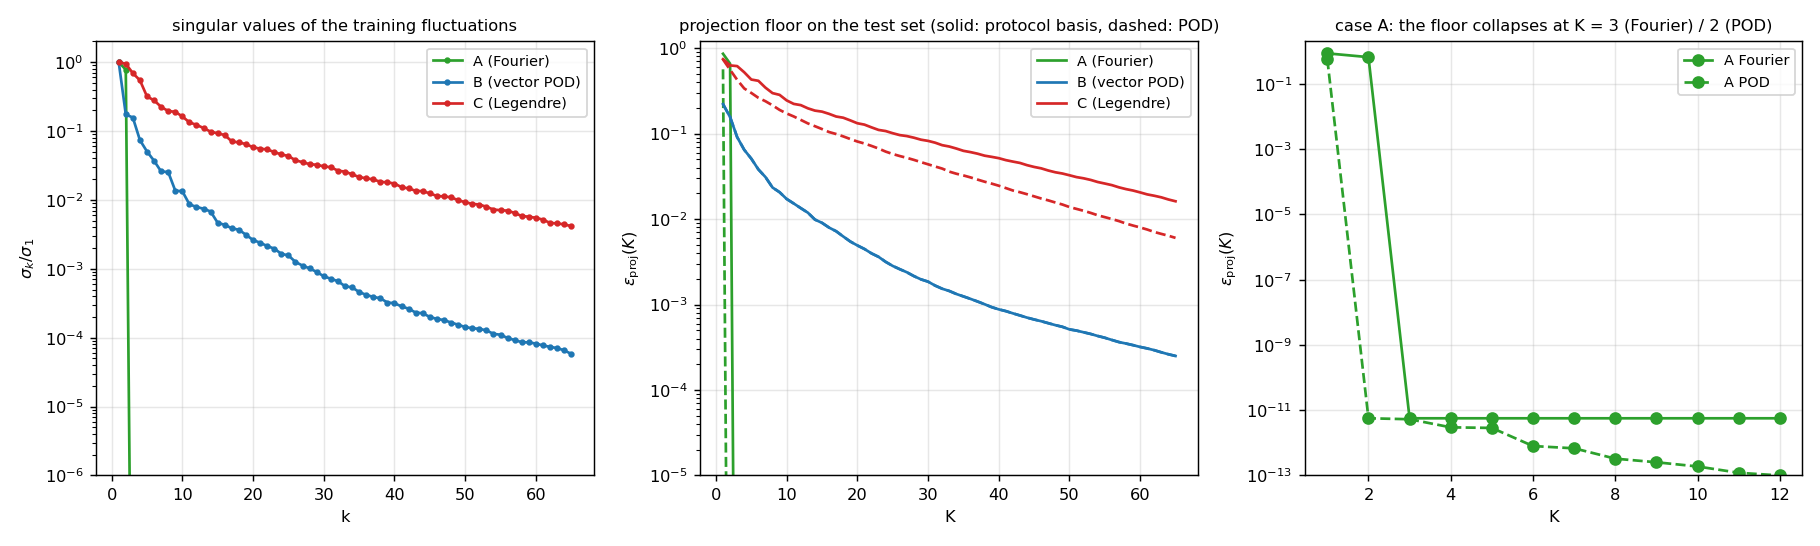
\includegraphics[width=0.90\textwidth,height=0.215\textheight,keepaspectratio]{fig1_spectra_floors.png}
  \caption{A priori spectral characterization of the three PDE benchmarks before any neural network training. \textbf{Left:} singular values $\sigma_k/\sigma_1$ of the centred training snapshots (empirical Kolmogorov $n$-width decay). \textbf{Centre:} test-set projection floor $\varepsilon_{\mathrm{proj}}(K)$ for the protocol basis (solid: Fourier in A, vector POD in B, discrete-QR Legendre in C) and for the optimal empirical POD basis (dashed). \textbf{Right:} zoom on Case~A, where the projection floor drops to numerical round-off ($\sim 6\cdot 10^{-12}$) at $K=2$ for POD and $K=3$ for Fourier (whose first mode $1/\sqrt{2}$ is constant).}
  \label{fig:rq2_fig1}
\end{figure}

\begin{table}[!htbp]
\centering
\caption{Test-set relative projection floor $\varepsilon_{\mathrm{proj}}(K) = \norm{(y-\bar{y}) - P_K(y-\bar{y})}_w / \norm{y}_w$ across modal truncation levels $K$ for the protocol basis and the empirical training POD basis. Multiply by $c_A = 0.1686$, $c_B = 0.0480$, or $c_C = 0.3484$ to convert $\varepsilon_{\mathrm{proj}}(K)$ into test $\NRMSE$.}
\label{tab:projection_floors}
\small\resizebox{\textwidth}{!}{%

\begin{tabular}{@{}rlllll@{}}
\toprule
\textbf{Modes $K$} & \textbf{Case A (Fourier)} & \textbf{Case A (POD)} & \textbf{Case B (Vector POD)} & \textbf{Case C (Legendre)} & \textbf{Case C (POD)} \\
\midrule
$1$  & $0.8596$ & $0.5649$ & $0.2215$ & $0.7432$ & $0.7371$ \\
$2$  & $0.6581$ & $5.66\cdot 10^{-12}$ & $0.1563$ & $0.6280$ & $0.5587$ \\
$3$  & $5.66\cdot 10^{-12}$ & $5.30\cdot 10^{-12}$ & $0.0910$ & $0.6166$ & $0.4261$ \\
$5$  & $5.66\cdot 10^{-12}$ & $2.87\cdot 10^{-12}$ & $0.0509$ & $0.4294$ & $0.2991$ \\
$9$  & $5.66\cdot 10^{-12}$ & $2.55\cdot 10^{-13}$ & $0.0206$ & $0.2841$ & $0.1895$ \\
$10$ & $5.66\cdot 10^{-12}$ & $1.89\cdot 10^{-13}$ & $0.0172$ & $0.2447$ & $0.1721$ \\
$12$ & $5.66\cdot 10^{-12}$ & $1.00\cdot 10^{-13}$ & $0.0134$ & $0.2155$ & $0.1447$ \\
$17$ & $5.66\cdot 10^{-12}$ & $2.53\cdot 10^{-14}$ & $0.00721$ & $0.1585$ & $0.0989$ \\
$33$ & $5.66\cdot 10^{-12}$ & $2.39\cdot 10^{-15}$ & $0.00144$ & $0.0706$ & $0.0359$ \\
$65$ & $5.66\cdot 10^{-12}$ & $1.24\cdot 10^{-15}$ & $2.50\cdot 10^{-4}$ & $0.0162$ & $0.00603$ \\
\midrule
Smallest $K$ for $\varepsilon_{\mathrm{proj}} \le 10\%$ & $3$ & $2$ & $3$ & $26$ & $17$ \\
Smallest $K$ for $\varepsilon_{\mathrm{proj}} \le 5\%$  & $3$ & $2$ & $6$ & $41$ & $28$ \\
Smallest $K$ for $\varepsilon_{\mathrm{proj}} \le 1\%$  & $3$ & $2$ & $14$ & $>65$ & $57$ \\
\bottomrule
\end{tabular}
}
\end{table}

Table~\ref{tab:projection_floors} reveals three sharply contrasting approximation regimes:
\begin{enumerate}[leftmargin=2em]
  \item \textbf{Case A is finite-rank and exactly modal:} Only two singular values are non-zero ($\sigma_2/\sigma_1 = 0.78$, $\sigma_3/\sigma_1 \approx 10^{-11}$). Because the protocol orders the Fourier basis starting with the spatially constant mode $\varphi_1(x) = 1/\sqrt{2}$ (which carries zero energy once the zero-wavenumber mean field is subtracted), $K=2$ spans $\{1/\sqrt{2}, \cos(\pi x)\}$ and omits $\sin(\pi x)$ ($\varepsilon_{\mathrm{proj}}(2) = 0.658$). At $K=3$, both $\cos(\pi x)$ and $\sin(\pi x)$ are included and $\varepsilon_{\mathrm{proj}}(K)$ collapses to $5.66\cdot 10^{-12}$ for all $K \ge 3$.
  \item \textbf{Case B exhibits rapid exponential POD decay:} Despite the nonlinear convective term $(\mathbf{v}\cdot\nabla)\mathbf{v}$ and the lid-corner velocity discontinuities, the cavity flow is confined to a fixed geometry where viscosity smooths the interior vorticity field. The singular values decay geometrically as $\sigma_k/\sigma_1 \sim e^{-0.1 k}$ ($\sigma_2/\sigma_1 = 0.175$, $\sigma_5/\sigma_1 = 0.050$, $\sigma_{10}/\sigma_1 = 0.013$, $\sigma_{17}/\sigma_1 = 0.0039$, $\sigma_{65}/\sigma_1 = 5.8\cdot 10^{-5}$). Just $K=6$ POD modes capture $95\%$ of the relative field norm ($\varepsilon_{\mathrm{proj}}(6) \le 0.05$, corresponding to $\NRMSE \le 2.4\cdot 10^{-3}$), $K=17$ modes give $\varepsilon_{\mathrm{proj}}(17) = 7.21\cdot 10^{-3}$ ($\NRMSE = 3.46\cdot 10^{-4}$), and $K=65$ modes give $\varepsilon_{\mathrm{proj}}(65) = 2.50\cdot 10^{-4}$ ($\NRMSE = 1.20\cdot 10^{-5}$). Thus, linear spatial reconstruction is not a bottleneck in Case~B.
  \item \textbf{Case C exhibits the classic Kolmogorov $n$-width barrier of travelling fronts:} The leading singular values remain nearly flat ($\sigma_2/\sigma_1 = 0.94$, $\sigma_3/\sigma_1 = 0.69$, $\sigma_5/\sigma_1 = 0.32$, $\sigma_{10}/\sigma_1 = 0.16$), and between $k=10$ and $k=65$ they decay by a factor of only $39$ (compared with $230$ in Case~B). Reaching a $5\%$ relative projection floor requires $K = 28$ optimal POD modes or $K = 41$ Legendre polynomials; at $K = 33$, the Legendre floor is still $\varepsilon_{\mathrm{proj}}(33) = 0.0706$ ($\NRMSE = 2.46\cdot 10^{-2}$), and even for an ideal $12$-dimensional linear subspace ($d_s^* = 12$), the POD rank floor is $\varepsilon_{\mathrm{rank}}(12) = 0.1447$ ($\NRMSE = 5.04\cdot 10^{-2}$).
\end{enumerate}
Crucially, projection floors provide \textbf{necessary} conditions for accuracy, never sufficient ones: they prove a priori that no linear decoder with $d_s \le 12$ can reach $\NRMSE < 5\cdot 10^{-2}$ in Case~C, whereas whether a modal decoder can actually approach its tiny floor in Case~B depends on the latent dynamics $\NNdyn$ and the optimizer.

\section{Part I: Reconstructor Nonlinearity Ablation (\texttt{RQ2})}
\label{sec:rq2}

In our first experimental campaign (\texttt{RQ2}), we hold the dynamics architecture $\NNdyn$, data splits, loss functions, and two-stage Adam+BFGS optimizer schedule fixed, and systematically replace $\NNrec$ across the hierarchy $\mathrm{L0} \to \mathrm{L1} \to \mathrm{L2} \to \mathrm{L3}$ under both frozen-latent ($\mathrm{R1}$) and end-to-end ($\mathrm{R2}$) training regimes. Across the three PDE benchmarks, the sweep covers $d_s \in \{1,2,3,5\}$ and $K \in \{d_s, 3, 5, 9, 17, 33, 65\}$ in Case~A (348 runs), $d_s \in \{1,5,10\}$ and $K \in \{d_s, 3, 5, 9, 17\}$ in Case~B (195 runs), and $d_s \in \{1,2,3,5,12\}$ and $K \in \{d_s, 5, 17, 33\}$ in Case~C (273 runs), with 3 random seeds $\{0,1,2\}$ per configuration, totalling \textbf{816 trained models}.

\subsection{Experimental Protocol and Statistical Reporting}

In \texttt{RQ2}, training uses Adam with learning rate $10^{-2}$ followed by \texttt{scipy} BFGS: 50 Adam + 150 BFGS epochs in Case~A (matching the original notebook), and 200 Adam + 500 BFGS epochs in Cases~B and~C (a reduced budget adopted so that the 468 runs of Cases~B and~C could be completed on a single workstation; the full $10{,}000$-iteration BFGS regime is the subject of Part~II in Section~\ref{sec:rq2bis}). For every procedure (a pair of variant $\mathrm{L}m$ and regime $\mathrm{R}j$), the best configuration $(d_s, K)$ is selected strictly on the \textbf{validation set} median NRMSE; the test set is never used for model selection. Because three seeds do not permit parametric hypothesis tests with statistical power below $p = 0.10$ (the minimum two-sided permutation $p$-value of two disjoint triples is $2/\binom{6}{3} = 0.10$), we report the median across the three seeds, the full range $[\min, \max]$, the ratio of medians relative to $\mathrm{L0}$, and whether the three seeds of a procedure are \emph{completely separated} from the three seeds of $\mathrm{L0}$.

\subsection{Case A Results: Smooth Periodic Dynamics and Curved Latent Coordinates}

Table~\ref{tab:rq2_caseA} summarises the validation-selected best configurations, the $d_s$-sweep of $\mathrm{L0}$ and $\mathrm{L1}$, and the $K$-sweep of $\mathrm{L2}$ and $\mathrm{L3}$ at $d_s = 3$ for Case~A.

\begin{table}[!htbp]
\centering
\caption{Case A (\texttt{ADR-1b}) results in \texttt{RQ2} (50 Adam + 150 BFGS epochs). \textbf{Top:} best configuration of each procedure selected on validation NRMSE (median and $[\min,\max]$ over 3 seeds). \textbf{Bottom:} test NRMSE across the modal truncation sweep $K$ at $d_s = 3$, together with the parameter-matched hidden width $w_g$ of $\mathrm{L3}$.}
\label{tab:rq2_caseA}
\small\resizebox{\textwidth}{!}{%

\begin{tabular}{@{}lrrrlrrlrr@{}}
\toprule
\textbf{Procedure} & $d_s$ & $K$ & $P_{\mathrm{rec}}$ & \textbf{Test NRMSE $[\min, \max]$} & $1-\rho$ & $\varepsilon_{\mathrm{total}}$ & \textbf{Ratio to L0} & \textbf{Separated} & \textbf{Train [s] / Infer [ms]} \\
\midrule
$\mathrm{L0}$ (R2) & $5$ & -- & $113$ & $2.26\cdot 10^{-2}$ $[1.96, 2.65]\cdot 10^{-2}$ & $9.05\cdot 10^{-3}$ & $0.134$ & $1.00$ & -- & $14.3$ / $14.7$ \\
$\mathrm{L1}$-R1 & $1$ & $1$ & $0$ & $1.68\cdot 10^{-1}$ $[1.64, 1.80]\cdot 10^{-1}$ & $6.30\cdot 10^{-1}$ & $0.995$ & $7.41$ & yes (worse) & $0.0$ / $0.3$ \\
$\mathrm{L1}$-R2 & $3$ & $3$ & $0$ & $2.85\cdot 10^{-2}$ $[2.57, 2.88]\cdot 10^{-2}$ & $1.35\cdot 10^{-2}$ & $0.169$ & $1.26$ & no & $3.8$ / $1.7$ \\
$\mathrm{L2}$-R1 & $5$ & $3$ & $18$ & $1.02\cdot 10^{-1}$ $[1.01, 1.02]\cdot 10^{-1}$ & $2.02\cdot 10^{-1}$ & $0.607$ & $4.52$ & yes (worse) & $0.0$ / $1.0$ \\
$\mathbf{L2}$\textbf{-R2} & $\mathbf{3}$ & $\mathbf{5}$ & $\mathbf{20}$ & $\mathbf{9.72\cdot 10^{-3}}$ $[9.26\cdot 10^{-3}, 1.36\cdot 10^{-2}]$ & $\mathbf{1.65\cdot 10^{-3}}$ & $\mathbf{0.058}$ & $\mathbf{0.43}$ & \textbf{yes (better)} & $\mathbf{4.1}$ / $\mathbf{1.8}$ \\
$\mathrm{L3}$-R1 & $3$ & $3$ & $87$ & $2.30\cdot 10^{-2}$ $[2.23, 2.42]\cdot 10^{-2}$ & $9.32\cdot 10^{-3}$ & $0.136$ & $1.01$ & no & $2.0$ / $3.6$ \\
$\mathrm{L3}$-R2 & $3$ & $17$ & $92$ & $1.18\cdot 10^{-2}$ $[1.09, 1.90]\cdot 10^{-2}$ & $2.43\cdot 10^{-3}$ & $0.070$ & $0.52$ & yes (better) & $5.5$ / $3.6$ \\
\bottomrule
\end{tabular}
}

\vspace{0.6em}\resizebox{\textwidth}{!}{%

\begin{tabular}{@{}lcccccc@{}}
\toprule
\textbf{K-Sweep at $d_s = 3$} & $K = 3$ & $K = 5$ & $K = 9$ & $K = 17$ & $K = 33$ & $K = 65$ \\
\midrule
$\mathrm{L2}$-R2 (end-to-end affine) & $1.32\cdot 10^{-2}$ & $9.72\cdot 10^{-3}$ & $1.03\cdot 10^{-2}$ & $1.36\cdot 10^{-2}$ & $1.20\cdot 10^{-2}$ & $1.20\cdot 10^{-2}$ \\
$\mathrm{L2}$-R1 (frozen $\mathrm{L0}$ latents) & $1.04\cdot 10^{-1}$ & $1.04\cdot 10^{-1}$ & $1.04\cdot 10^{-1}$ & $1.04\cdot 10^{-1}$ & $1.04\cdot 10^{-1}$ & $1.04\cdot 10^{-1}$ \\
$\mathrm{L3}$-R2 (end-to-end MLP) & $1.65\cdot 10^{-2}$ & $1.48\cdot 10^{-2}$ & $1.98\cdot 10^{-2}$ & $1.18\cdot 10^{-2}$ & $9.55\cdot 10^{-2}$ & $9.55\cdot 10^{-2}$ \\
$\mathrm{L3}$-R1 (frozen $\mathrm{L0}$ latents) & $2.30\cdot 10^{-2}$ & $2.32\cdot 10^{-2}$ & $2.45\cdot 10^{-2}$ & $4.23\cdot 10^{-2}$ & $1.07\cdot 10^{-1}$ & $1.07\cdot 10^{-1}$ \\
Matched hidden width $w_g$ of $\mathrm{L3}$ & $6$ & $5$ & $4$ & $3$ & $1$ & $1$ \\
\bottomrule
\end{tabular}
}
\end{table}

Four key findings emerge from Case~A:
\begin{enumerate}[leftmargin=2em]
  \item \textbf{End-to-end affine reconstruction ($\mathrm{L2}$-R2) beats $\mathrm{L0}$ by $2.3\times$ with $5.6\times$ fewer parameters:} Once $K \ge 3$ includes $\cos(\pi x)$ and $\sin(\pi x)$, $\mathrm{L2}$-R2 reaches $\NRMSE = 9.72\cdot 10^{-3}$ ($P_{\mathrm{rec}} = 20$), compared with $2.26\cdot 10^{-2}$ for $\mathrm{L0}$ ($P_{\mathrm{rec}} = 113$). Across all paired configurations with $d_s \in \{2,3,5\}$ and $K \in \{3,5\}$, the paired ratio $\NRMSE_{\mathrm{L2\text{-}R2}}/\NRMSE_{\mathrm{L0}}$ lies between $0.44$ and $0.71$ in every seed, strongly supporting Hypothesis~H1 in Regime~R2. Furthermore, as predicted by Proposition~\ref{prop:rec_rank_bound}, the error of $\mathrm{L2}$-R2 is completely flat from $K=3$ to $K=65$ ($1.0$--$1.4\cdot 10^{-2}$).
  \item \textbf{The latents learned by $\mathrm{L0}$ are information-complete but curved ($\mathrm{R1}$ vs.\ $\mathrm{R2}$):} When the exact same affine decoder $\mathrm{L2}$ is fitted to the frozen latent trajectories of $\mathrm{L0}$ ($\mathrm{L2}$-R1), its error jumps by an order of magnitude to $1.04\cdot 10^{-1}$ ($10.8\times$ worse than $\mathrm{L2}$-R2 and $4.0$--$4.4\times$ worse than $\mathrm{L0}$). Yet when the nonlinear modal decoder $\mathrm{L3}$ is fitted to those very same frozen latents ($\mathrm{L3}$-R1 at $K=3$), it recovers $\NRMSE = 2.30\cdot 10^{-2}$ (ratio $1.01$ to $\mathrm{L0}$)! Direct polynomial regression of the true Fourier coefficients $(a(t), b(t))$ on the learned $\mathrm{L0}$ latents $\mathbf{s}(t)$ explains why: a degree-1 (affine) fit achieves only $R^2 = 0.55$, a quadratic fit achieves $R^2 = 0.88$, and a cubic polynomial achieves $R^2 = 0.98$. As visualised in Figure~\ref{fig:rq2_fig9}, $\mathrm{L0}$ learns a smooth, invertible, but nonlinearly sheared coordinate chart of the $(\cos\pi x, \sin\pi x)$ amplitude plane, which is consistent across seeds up to an affine transformation (cross-seed alignment $R^2 \in [0.95, 0.99]$). Thus, in a smooth linear PDE, the nonlinearity of $\NNrec$ is not needed by the physics; it merely absorbs the curved coordinate chart chosen during joint optimization with $\NNdyn$.
  \item \textbf{Why $\mathrm{L3}$ collapses at $K \ge 33$:} Under the parameter-matching rule $P_{\mathrm{rec}}^{\mathrm{L3}}(w_g) \le P_{\mathrm{rec}}^{\mathrm{L0}} = 106$ (at $d_s=3$), the output layer of $g_\theta$ requires $(w_g + 1)K$ weights. For $K \in \{33, 65\}$, this forces the hidden width $w_g$ down to \textbf{a single neuron} ($w_g = 1$), creating a rank-1 bottleneck inside $g_\theta$ that causes $\mathrm{L3}$-R2 and $\mathrm{L3}$-R1 to jump to $\NRMSE \approx 0.10$.
\end{enumerate}

\begin{figure}[!htbp]
  \centering
  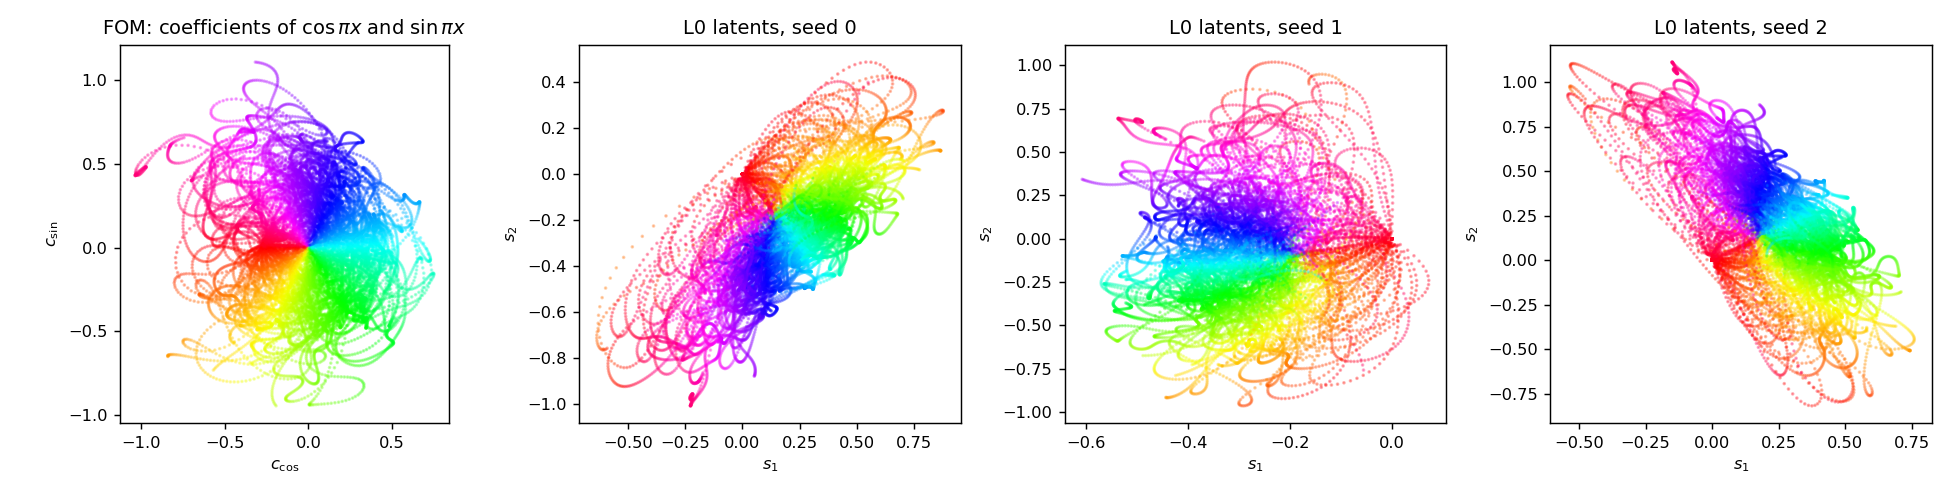
\includegraphics[width=0.90\textwidth,height=0.215\textheight,keepaspectratio]{fig9_A_latents.png}
  \caption{Curved latent coordinates learned by $\mathrm{L0}$ in Case~A ($d_s = 2$). \textbf{Left:} true Fourier coefficients $(c_{\cos}, c_{\sin})$ of the centred test fields, coloured by phase angle. \textbf{Right:} learned latent trajectories $(s_1(t), s_2(t))$ of $\mathrm{L0}$ across the three random seeds $\{0,1,2\}$ for the exact same test states and colour map. The circular modal phase space is preserved topologically but sheared and radially compressed by a cubic distortion ($R^2_{\mathrm{lin}} = 0.55$, cubic $R^2 = 0.98$).}
  \label{fig:rq2_fig9}
\end{figure}

\subsection{Case B Results: Navier--Stokes Cavity Flow, Quiescent Corners, and Preconditioning}

Table~\ref{tab:rq2_caseB} reports the \texttt{RQ2} results for the 2D lid-driven cavity flow at the 200 Adam + 500 BFGS budget.

\begin{table}[!htbp]
\centering
\caption{Case B (\texttt{2D-Stokes}) results in \texttt{RQ2} (200 Adam + 500 BFGS epochs). \textbf{Top:} validation-selected best configuration of each procedure and goal-oriented physical metrics (direction error, relative vorticity error, and time-extrapolation ratio $\varepsilon_{[20,40]}/\varepsilon_{[0,20]}$). \textbf{Bottom:} $K$-sweep at $d_s = 10$.}
\label{tab:rq2_caseB}
\footnotesize\resizebox{\textwidth}{!}{%

\begin{tabular}{@{}lrrrlrrrrrr@{}}
\toprule
\textbf{Procedure} & $d_s$ & $K$ & $P_{\mathrm{rec}}$ & \textbf{Test NRMSE $[\min, \max]$} & \textbf{Ratio L0} & \textbf{Dir.\ Err.} & \textbf{Vort.\ Err.} & \textbf{Extrap.} & \textbf{Train [s]} & \textbf{Infer [ms]} \\
\midrule
$\mathrm{L0}$ (R2) & $10$ & -- & $2186$ & $1.97\cdot 10^{-2}$ $[1.89, 2.25]\cdot 10^{-2}$ & $1.00$ & $0.051$ & $0.887$ & $0.974$ & $240.0$ & $931.9$ \\
$\mathrm{L1}$-R1 & $1$ & $1$ & $0$ & $3.66\cdot 10^{-2}$ $[2.93, 6.02]\cdot 10^{-2}$ & $1.86$ & $0.323$ & $0.765$ & $0.980$ & $0.0$ & $12.3$ \\
$\mathrm{L1}$-R2 & $5$ & $5$ & $0$ & $8.69\cdot 10^{-3}$ $[7.92, 9.16]\cdot 10^{-3}$ & $0.44$ & $0.048$ & $0.241$ & $0.968$ & $38.4$ & $8.0$ \\
$\mathrm{L2}$-R1 & $10$ & $5$ & $60$ & $1.53\cdot 10^{-2}$ $[1.39, 1.77]\cdot 10^{-2}$ & $0.77$ & $0.098$ & $0.411$ & $1.007$ & $28.0$ & $8.4$ \\
$\mathrm{L2}$-R2 & $5$ & $17$ & $119$ & $8.06\cdot 10^{-3}$ $[7.98, 8.91]\cdot 10^{-3}$ & $0.41$ & $0.028$ & $0.232$ & $1.065$ & $46.0$ & $10.2$ \\
$\mathbf{L3}$\textbf{-R1} & $\mathbf{10}$ & $\mathbf{10}$ & $\mathbf{2134}$ & $\mathbf{4.43\cdot 10^{-3}}$ $[4.21, 4.51]\cdot 10^{-3}$ & $\mathbf{0.22}$ & $\mathbf{0.026}$ & $\mathbf{0.110}$ & $\mathbf{0.774}$ & $\mathbf{92.0}$ & $\mathbf{12.7}$ \\
$\mathbf{L3}$\textbf{-R2} & $\mathbf{10}$ & $\mathbf{10}$ & $\mathbf{2134}$ & $\mathbf{4.52\cdot 10^{-3}}$ $[4.27, 4.72]\cdot 10^{-3}$ & $\mathbf{0.23}$ & $\mathbf{0.025}$ & $\mathbf{0.123}$ & $\mathbf{0.747}$ & $\mathbf{110.2}$ & $\mathbf{10.4}$ \\
\bottomrule
\end{tabular}
}

\vspace{0.6em}\resizebox{\textwidth}{!}{%

\begin{tabular}{@{}lccccc@{}}
\toprule
\textbf{K-Sweep at $d_s = 10$} & $K = 3$ & $K = 5$ & $K = 9$ & $K = 10$ & $K = 17$ \\
\midrule
$\mathrm{L2}$-R2 test NRMSE ($\eta = \varepsilon_{\mathrm{total}}/\varepsilon_{\mathrm{proj}}$) & $1.23\cdot 10^{-2}$ ($2.8$) & $9.75\cdot 10^{-3}$ ($4.0$) & $1.00\cdot 10^{-2}$ ($10.2$) & $8.07\cdot 10^{-3}$ ($9.8$) & $8.99\cdot 10^{-3}$ ($26.0$) \\
$\mathrm{L2}$-R1 test NRMSE (frozen $\mathrm{L0}$ latents) & $1.71\cdot 10^{-2}$ & $1.53\cdot 10^{-2}$ & $1.69\cdot 10^{-2}$ & $1.69\cdot 10^{-2}$ & $1.66\cdot 10^{-2}$ \\
$\mathrm{L3}$-R2 test NRMSE ($\eta = \varepsilon_{\mathrm{total}}/\varepsilon_{\mathrm{proj}}$) & $1.15\cdot 10^{-2}$ ($2.6$) & $1.07\cdot 10^{-2}$ ($4.4$) & $5.16\cdot 10^{-3}$ ($5.2$) & $4.52\cdot 10^{-3}$ ($5.5$) & $4.74\cdot 10^{-3}$ ($13.7$) \\
$\mathrm{L3}$-R1 test NRMSE (frozen $\mathrm{L0}$ latents) & $1.00\cdot 10^{-2}$ & $6.38\cdot 10^{-3}$ & $5.05\cdot 10^{-3}$ & $4.43\cdot 10^{-3}$ & $4.75\cdot 10^{-3}$ \\
Matched hidden width $w_g$ of $\mathrm{L3}$ & $39$ & $38$ & $36$ & $36$ & $33$ \\
\bottomrule
\end{tabular}
}
\end{table}

At the 500-BFGS-epoch budget of \texttt{RQ2}, replacing the pointwise MLP $\mathrm{L0}$ ($1.97\cdot 10^{-2}$) with vector POD modes yields dramatic gains across all modal variants: even the parameter-free identity $\mathrm{L1}$-R2 reaches $8.69\cdot 10^{-3}$ ($2.3\times$ lower error than $\mathrm{L0}$), the affine map $\mathrm{L2}$-R2 reaches $8.06\cdot 10^{-3}$ ($2.4\times$ lower error with $18\times$ fewer decoder parameters), and the nonlinear coefficient map $\mathrm{L3}$ reaches $4.52\cdot 10^{-3}$ in R2 and $4.43\cdot 10^{-3}$ in R1 ($4.4\times$ lower NRMSE and $8\times$ lower vorticity error than $\mathrm{L0}$, while accelerating test-set decoder evaluation by $90\times$, from $932$~ms to $10.4$~ms). However, notice that for $K \ge 10$, the efficiency ratios $\eta = \varepsilon_{\mathrm{total}}/\varepsilon_{\mathrm{proj}}(K)$ are large ($9.8$--$26.0$ for $\mathrm{L2}$, $5.5$--$13.7$ for $\mathrm{L3}$): the POD basis is already capable of $\NRMSE \le 8\cdot 10^{-4}$, so both the small canonical $7\text{--}7$ dynamics network and the 500-iteration BFGS cap limit accuracy---a diagnosis that \texttt{RQ2-bis} confirms and resolves in Section~\ref{sec:rq2bis}.

\begin{figure}[!htbp]
  \centering
  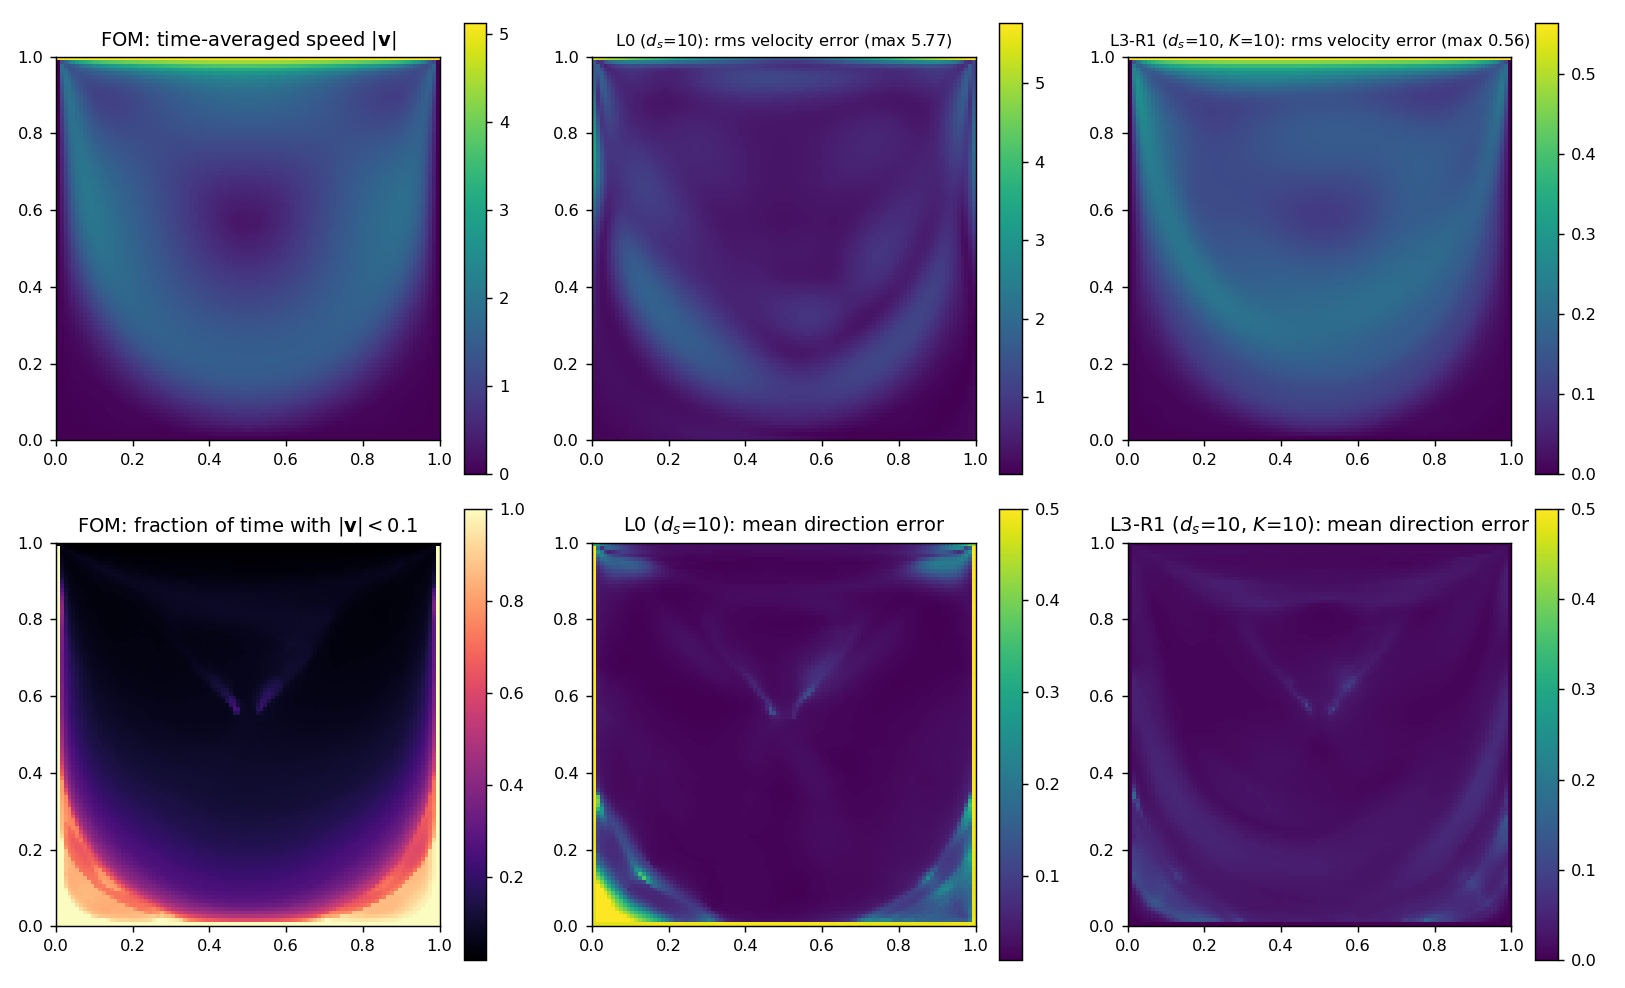
\includegraphics[width=0.90\textwidth,height=0.215\textheight,keepaspectratio]{fig8_B_maps.png}
  \caption{Spatial anatomy of velocity and direction errors in Case~B ($d_s = 10$, test set). \textbf{Top row:} time-averaged speed $\norm{\mathbf{v}}_2$ of the true FOM flow (left), and pointwise rms velocity error of $\mathrm{L0}$ (centre, max $0.68$) and $\mathrm{L3}$-R1 (right, max $0.17$). \textbf{Bottom row:} fraction of time steps where the true speed is below $0.1$ (left), and time-averaged direction error $\norm{\mathbf{d}(\hat{\mathbf{v}}) - \mathbf{d}(\mathbf{v})}^2$ of $\mathrm{L0}$ (centre) and $\mathrm{L3}$-R1 (right).}
  \label{fig:rq2_fig8}
\end{figure}

Figure~\ref{fig:rq2_fig8} resolves Hypothesis~H3 regarding where the direction error~\eqref{eq:caseB_loss} originates. Because the unit-vector map $\mathbf{d}(\mathbf{v}) = \mathbf{v}/(10^{-4} + \norm{\mathbf{v}})$ has Jacobian scaling as $1/\norm{\mathbf{v}}$, it is ill-conditioned wherever the flow speed $\norm{\mathbf{v}}$ is small: $22.0\%$ of space-time test points have speed $\norm{\mathbf{v}} < 0.1$ (compared with lid speeds of order $10$), yet they account for \textbf{$77.0\%$ of the total direction error in $\mathrm{L0}$ and $89.5\%$ in $\mathrm{L3}$-R1} (points with $\norm{\mathbf{v}} < 0.01$ alone carry $54.4\%$ and $47.3\%$). Consequently, the direction error is concentrated not at the two upper singular lid corners (which carry only $6.9\%$ of the direction error in $\mathrm{L0}$ and $1.4\%$ in $\mathrm{L3}$-R1), but rather in the quiescent bottom strip of the cavity ($30.6\%$ and $16.5\%$), along the stationary walls, at the zero-velocity centre of the primary vortex, and along the separatrix between the primary and secondary corner vortices.

\subsection{Case C Results: Travelling Fronts, the Kolmogorov Barrier, and the Threshold at \texorpdfstring{$d_s = 3$}{ds = 3}}

Table~\ref{tab:rq2_caseC} and Figure~\ref{fig:rq2_fig7} present the \texttt{RQ2} results for the 1D Aliev--Panfilov electrophysiology benchmark.

\begin{table}[!htbp]
\centering
\caption{Case C (\texttt{AP1D}) results in \texttt{RQ2} (200 Adam + 500 BFGS epochs). \textbf{Top:} validation-selected best configuration of each procedure and front activation-time MAE (ms). \textbf{Bottom:} $K$-sweep at $d_s = 12$ and $d_s$-sweep of $\mathrm{L0}$ vs.\ $\mathrm{L1}$.}
\label{tab:rq2_caseC}
\footnotesize\resizebox{\textwidth}{!}{%

\begin{tabular}{@{}lrrrlrrlrrr@{}}
\toprule
\textbf{Procedure} & $d_s$ & $K$ & $P_{\mathrm{rec}}$ & \textbf{Test NRMSE $[\min, \max]$} & $\varepsilon_{\mathrm{total}}$ & \textbf{Ratio L0} & \textbf{Sep.} & \textbf{Act.\ MAE [ms]} & \textbf{Train [s]} & \textbf{Infer [ms]} \\
\midrule
$\mathbf{L0}$ \textbf{(R2)} & $\mathbf{5}$ & -- & $\mathbf{1361}$ & $\mathbf{1.76\cdot 10^{-2}}$ $[1.58, 3.27]\cdot 10^{-2}$ & $\mathbf{0.051}$ & $\mathbf{1.00}$ & -- & $\mathbf{1.00}$ $[0.92, 1.54]$ & $\mathbf{133.7}$ & $\mathbf{366.8}$ \\
$\mathrm{L1}$-R1 & $1$ & $1$ & $0$ & $3.15\cdot 10^{-1}$ $[3.02, 3.20]\cdot 10^{-1}$ & $0.904$ & $17.86$ & yes & $319.1$ & $0.0$ & $4.0$ \\
$\mathrm{L1}$-R2 & $12$ & $12$ & $0$ & $1.22\cdot 10^{-1}$ $[1.20, 1.32]\cdot 10^{-1}$ & $0.350$ & $6.92$ & yes & $8.35$ $[8.34, 8.42]$ & $22.5$ & $1.9$ \\
$\mathrm{L2}$-R1 & $12$ & $33$ & $429$ & $1.94\cdot 10^{-1}$ $[1.76, 2.12]\cdot 10^{-1}$ & $0.556$ & $10.99$ & yes & $26.56$ $[19.6, 45.4]$ & $16.0$ & $6.1$ \\
$\mathrm{L2}$-R2 & $12$ & $33$ & $429$ & $1.01\cdot 10^{-1}$ $[1.00, 1.03]\cdot 10^{-1}$ & $0.290$ & $5.73$ & yes & $5.10$ $[4.89, 5.38]$ & $27.5$ & $3.0$ \\
$\mathrm{L3}$-R1 & $12$ & $17$ & $1417$ & $6.62\cdot 10^{-2}$ $[6.36, 6.86]\cdot 10^{-2}$ & $0.190$ & $3.75$ & yes & $2.78$ $[2.70, 2.89]$ & $34.0$ & $14.2$ \\
$\mathrm{L3}$-R2 & $12$ & $17$ & $1417$ & $6.93\cdot 10^{-2}$ $[6.69, 7.02]\cdot 10^{-2}$ & $0.199$ & $3.93$ & yes & $2.80$ $[2.70, 2.97]$ & $51.7$ & $5.0$ \\
\bottomrule
\end{tabular}
}

\vspace{0.6em}\resizebox{\textwidth}{!}{%

\begin{tabular}{@{}lcccc@{\hspace{2em}}lccccc@{}}
\toprule
\textbf{K-Sweep ($d_s=12$)} & $K=5$ & $K=12$ & $K=17$ & $K=33$ & \textbf{$d_s$-Sweep} & $d_s=1$ & $d_s=2$ & $d_s=3$ & $d_s=5$ & $d_s=12$ \\
\midrule
$\mathrm{L2}$-R2 NRMSE & $0.159$ & $0.103$ & $0.102$ & $0.101$ & $\mathrm{L0}$ (R2) & $0.134$ & $0.120$ & $\mathbf{0.0176}$ & $\mathbf{0.0176}$ & $0.0221$ \\
$\mathrm{L2}$-R2 $\eta = \varepsilon/\varepsilon_{\mathrm{proj}}$ & $1.06$ & $1.38$ & $1.85$ & $4.11$ & $\mathrm{L1}$-R2 & $0.281$ & $0.252$ & $0.236$ & $0.166$ & $0.122$ \\
$\mathrm{L3}$-R2 NRMSE & $0.150$ & $0.0809$ & $0.0693$ & $0.0693$ & $\mathrm{L1}$-R1 & $0.315$ & $0.327$ & $0.385$ & $0.373$ & $0.365$ \\
$\mathrm{L3}$-R2 $\eta = \varepsilon/\varepsilon_{\mathrm{proj}}$ & $1.00$ & $1.08$ & $1.26$ & $2.82$ & Seed align $R^2$ ($\mathrm{L0}$) & $0.015$ & $0.641$ & $\mathbf{0.970}$ & $\mathbf{0.985}$ & $\mathbf{0.991}$ \\
\bottomrule
\end{tabular}
}
\end{table}

Case~C provides an unequivocal demonstration of why the non-separable pointwise MLP reconstructor $\mathrm{L0}$ was invented:
\begin{enumerate}[leftmargin=2em]
  \item \textbf{Complete failure of fixed-basis decoders ($\mathrm{L1}$--$\mathrm{L3}$) against moving fronts:} No fixed-basis reconstructor comes closer to $\mathrm{L0}$ ($1.76\cdot 10^{-2}$, relative error $\varepsilon_{\mathrm{total}} = 5.0\%$, activation-time MAE $1.00$~ms) than a factor of \textbf{$3.75\times$} ($\mathrm{L3}$-R1 at $6.62\cdot 10^{-2}$) or \textbf{$5.73\times$} ($\mathrm{L2}$-R2 at $1.01\cdot 10^{-1}$). As shown in Table~\ref{tab:rq2_caseC} (bottom left), $\mathrm{L2}$-R2 hugs the Legendre projection floor at $K=5$ ($\eta = 1.06$), slows down at $K=12$ ($\eta = 1.38$), and completely stagnates at $0.101$--$0.103$ for $K \in \{12, 17, 33\}$ ($\eta$ rising to $4.11$) because of the 12-dimensional rank bound $\varepsilon_{\mathrm{rank}}(12) = 0.1447$. Even when $\mathrm{L3}$ uses a parameter-matched nonlinear MLP $g_\theta(\mathbf{s})$ to curve the 12-dimensional manifold inside $V_K$, it is pinned directly against the Legendre projection floor up to $K=17$ ($\eta = 1.00$ at $K=5$, $1.08$ at $K=12$, $1.26$ at $K=17$) and stalls at $6.93\cdot 10^{-2}$ at $K=33$ as its matched hidden width shrinks from $30$ to $21$.
  \item \textbf{Sharp phase transition of $\mathrm{L0}$ at the intrinsic dimension $d_s = 3$:} As $d_s$ increases from $1$ to $2$ to $3$, the test NRMSE of $\mathrm{L0}$ drops abruptly by \textbf{$7\times$}, from $0.134$ ($d_s=1$) and $0.120$ ($d_s=2$) to \textbf{$1.76\cdot 10^{-2}$} at $d_s=3$ ($\varepsilon_{\mathrm{total}} = 0.050$, $8.5\times$ below the 3-mode POD rank floor $0.4261$!), and remains on a plateau for $d_s = 5$ ($1.76\cdot 10^{-2}$) and $d_s = 12$ ($2.21\cdot 10^{-2}$). Simultaneously, the cross-seed affine alignment $R^2$ between the latent trajectories of different seeds jumps from $0.015$ ($d_s=1$) and $0.641$ ($d_s=2$) to \textbf{$0.970$, $0.985$, and $0.991$} for $d_s = 3, 5, 12$. Three latent variables suffice to parameterise the positions and recovery states of the two colliding depolarisation waves, and $\NNrec(\mathbf{s},x)$ translates the steep wave profiles directly in $x$ as a function of $\mathbf{s}(t)$ without Gibbs oscillations (Figure~\ref{fig:rq2_fig7}).
\end{enumerate}

\begin{figure}[!htbp]
  \centering
  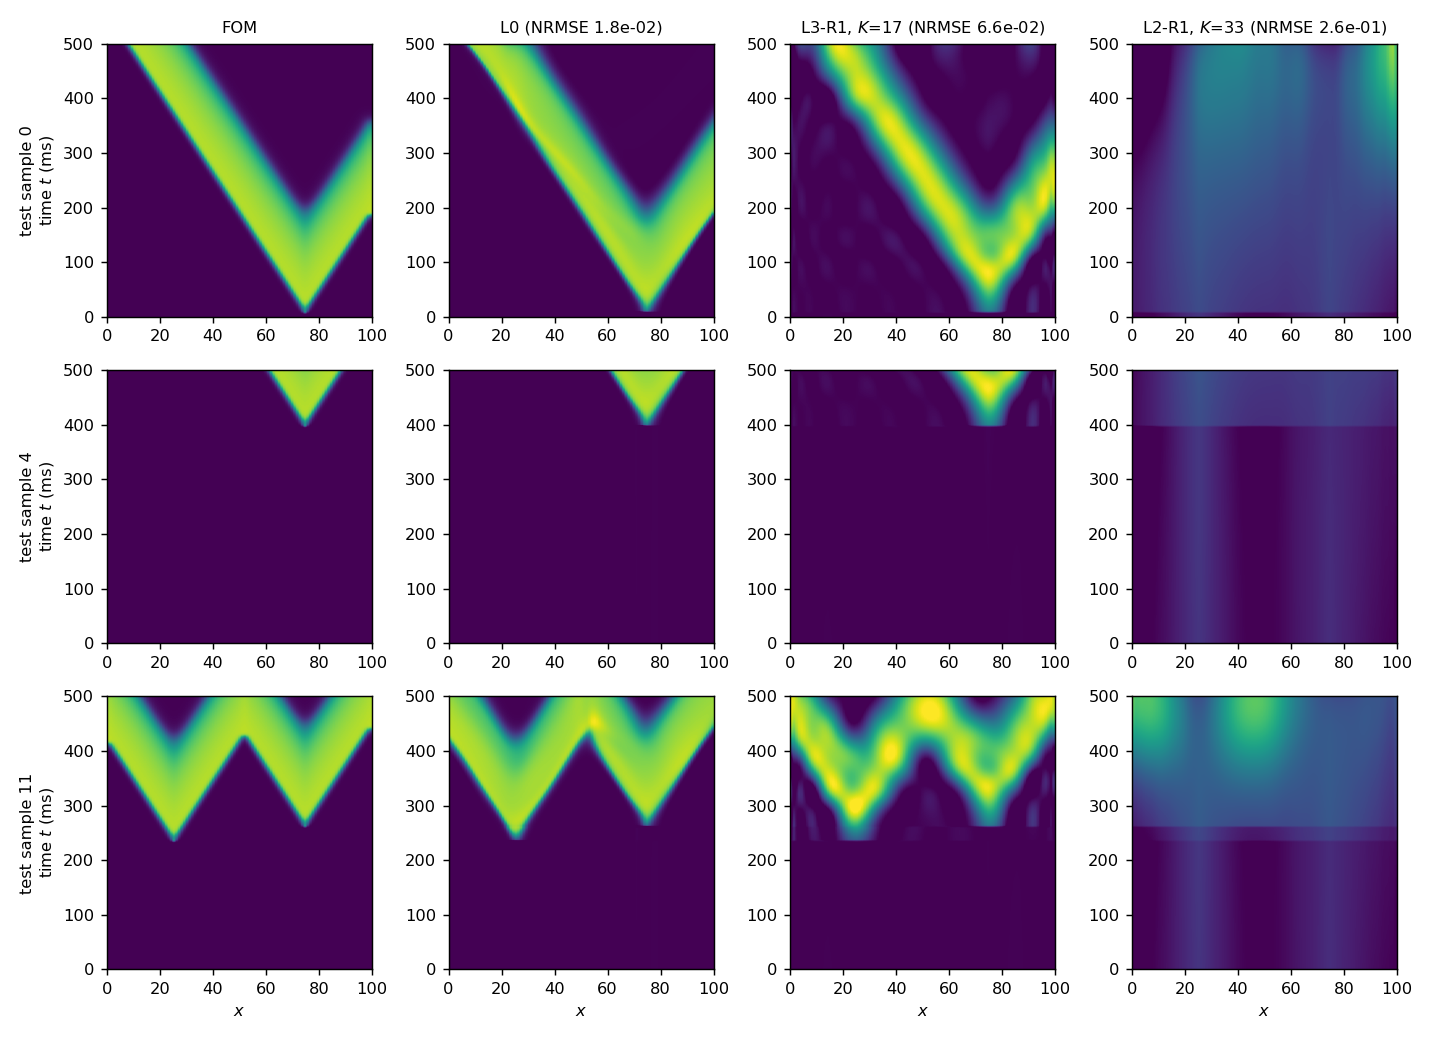
\includegraphics[width=0.90\textwidth,height=0.215\textheight,keepaspectratio]{fig7_C_decoders.png}
  \caption{Space-time transmembrane potential $y(x,t)$ across three test trajectories of Case~C (rows), decoded from the \emph{exact same frozen $\mathrm{L0}$ latent trajectory} ($d_s = 5$, Regime~R1). \textbf{Columns:} FOM ground truth; original implicit MLP $\mathrm{L0}$ ($\NRMSE = 1.76\cdot 10^{-2}$); nonlinear modal decoder $\mathrm{L3}$ ($K=17$, $\NRMSE = 6.62\cdot 10^{-2}$); and affine modal decoder $\mathrm{L2}$ ($K=33$, $\NRMSE = 1.94\cdot 10^{-1}$). The frozen $\mathrm{L0}$ latents trigger the wave onset at the exact right millisecond in every decoder, but fixed polynomial bases ($\mathrm{L2}, \mathrm{L3}$) smear the steep depolarisation fronts and introduce severe Gibbs ringing.}
  \label{fig:rq2_fig7}
\end{figure}

\subsection{Cross-Case Synthesis: Error vs.\ \texorpdfstring{$K$}{K}, Error vs.\ \texorpdfstring{$d_s$}{ds}, and Parameter Pareto Fronts}

Figures~\ref{fig:rq2_fig2}, \ref{fig:rq2_fig3}, and~\ref{fig:rq2_fig5} synthesise the 816 runs of \texttt{RQ2} across all three PDE benchmarks.

\begin{figure}[!htbp]
  \centering
  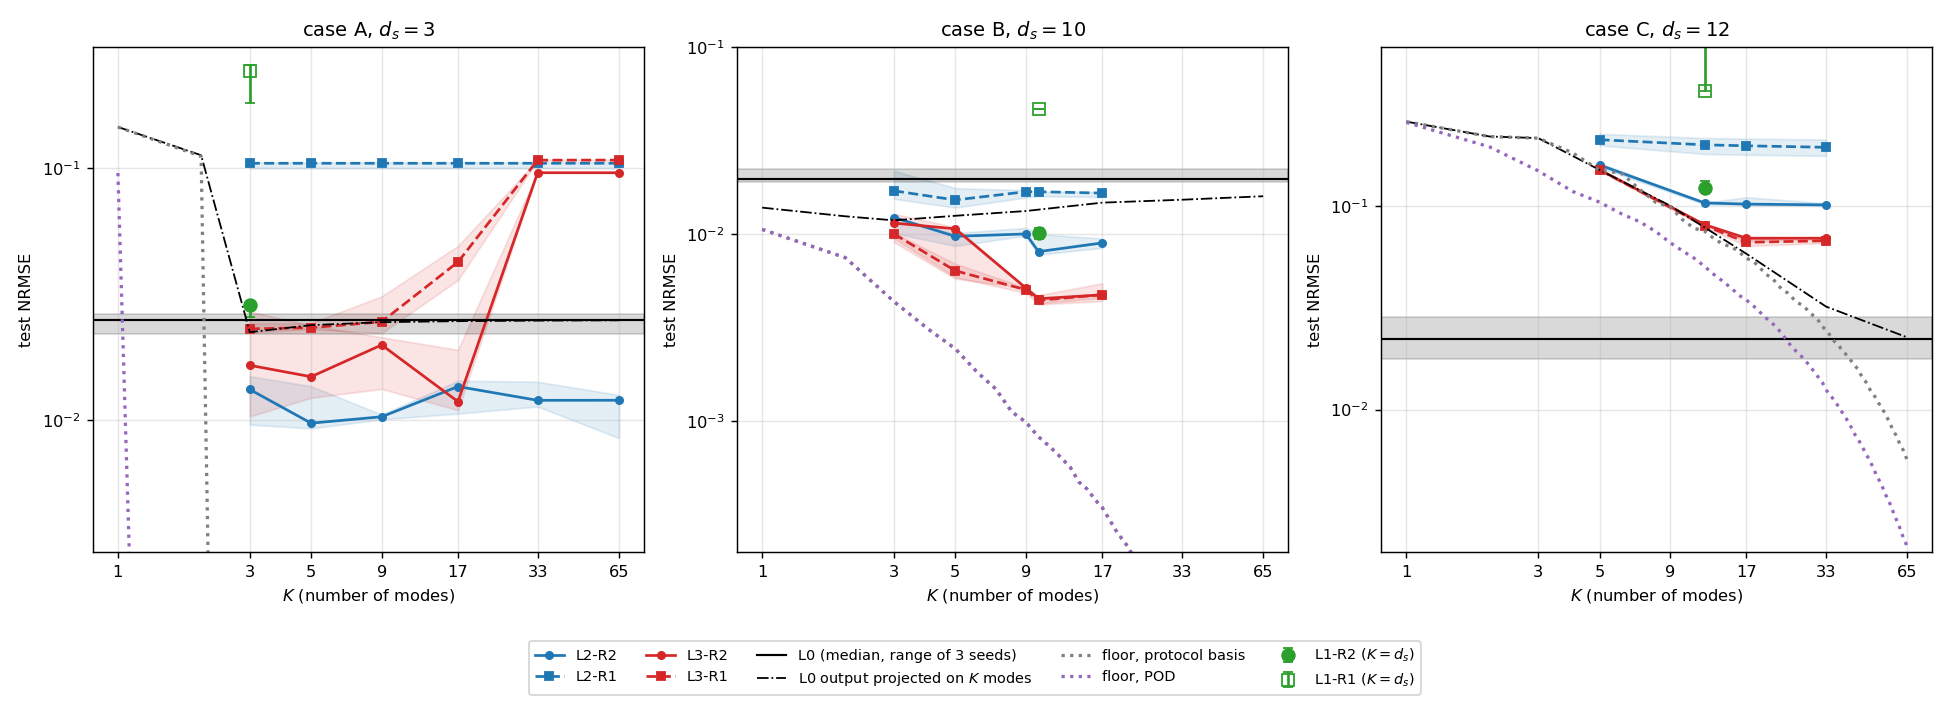
\includegraphics[width=0.90\textwidth,height=0.215\textheight,keepaspectratio]{fig2_error_vs_K.png}
  \caption{The core \texttt{RQ2} comparison: test NRMSE (median and min--max band over 3 seeds) against the number of basis modes $K$ at reference latent dimensions $d_s = 3$ (Case~A), $d_s = 10$ (Case~B), and $d_s = 12$ (Case~C). Solid lines denote end-to-end training ($\mathrm{R2}$) and dashed lines denote frozen-latent fitting ($\mathrm{R1}$) for $\mathrm{L2}$ (blue) and $\mathrm{L3}$ (red), alongside $\mathrm{L1}$ at $K=d_s$ (green), the $\mathrm{L0}$ seed band (grey shaded), the $\mathrm{L0}$ output orthogonally projected onto $K$ modes (black dash-dotted), and the projection floors $\varepsilon_{\mathrm{proj}}(K)$ (dotted).}
  \label{fig:rq2_fig2}
\end{figure}

\begin{figure}[!htbp]
  \centering
  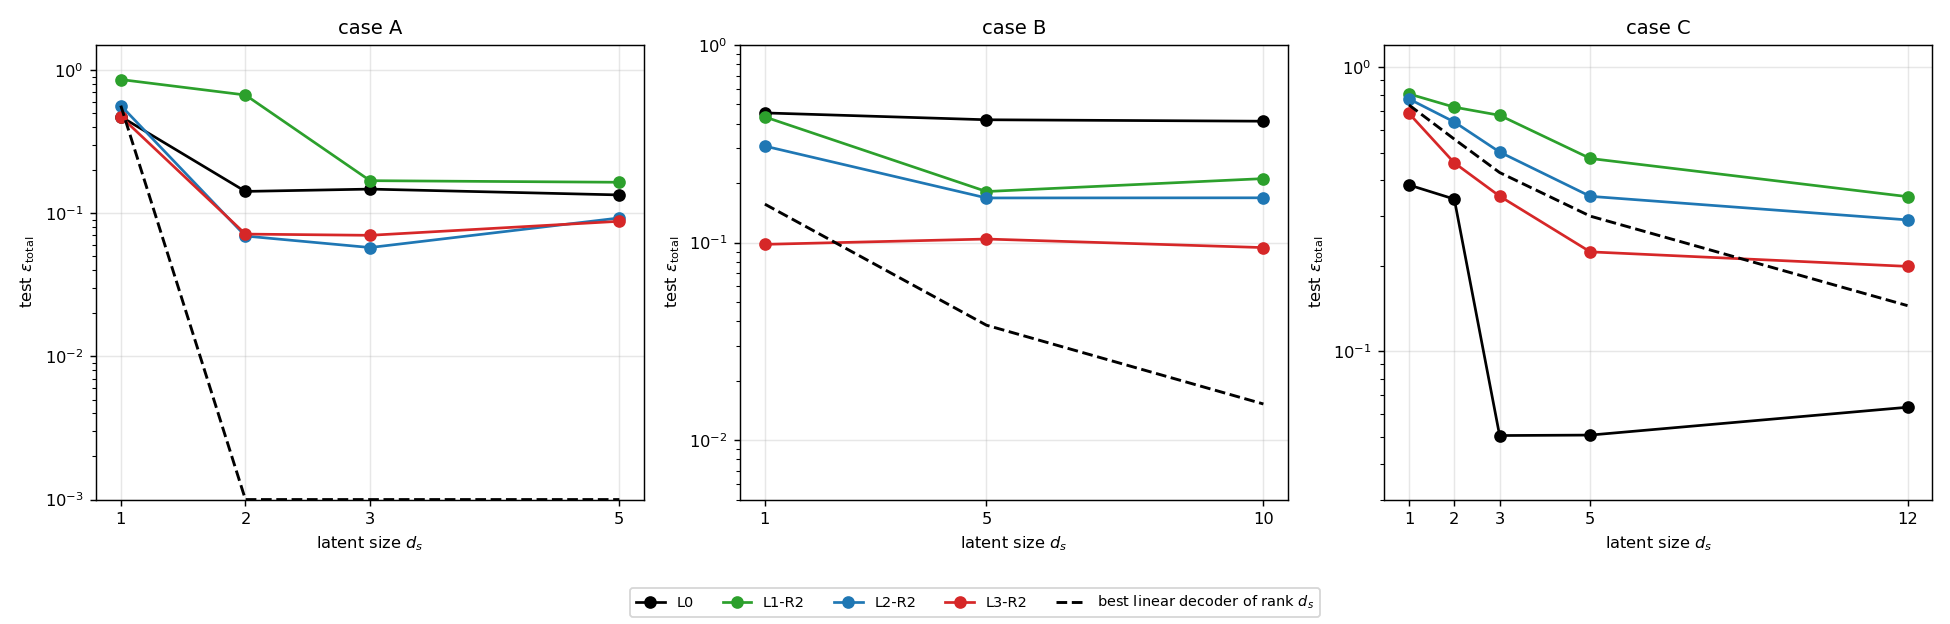
\includegraphics[width=0.90\textwidth,height=0.215\textheight,keepaspectratio]{fig3_rank_bound.png}
  \caption{Verification of the Reconstructor Rank Bound (Proposition~\ref{prop:rec_rank_bound}): relative test error $\varepsilon_{\mathrm{total}}$ against latent size $d_s$ for $\mathrm{L0}$, $\mathrm{L1}$-R2, $\mathrm{L2}$-R2, and $\mathrm{L3}$-R2 (with $K$ selected on validation), compared against the linear rank floor $\varepsilon_{\mathrm{rank}}(r)$ of the leading $r$ POD modes (black dashed; $r = d_s$ in Cases~A and~C, $r = d_s + 1$ in Case~B).}
  \label{fig:rq2_fig3}
\end{figure}

\begin{figure}[!htbp]
  \centering
  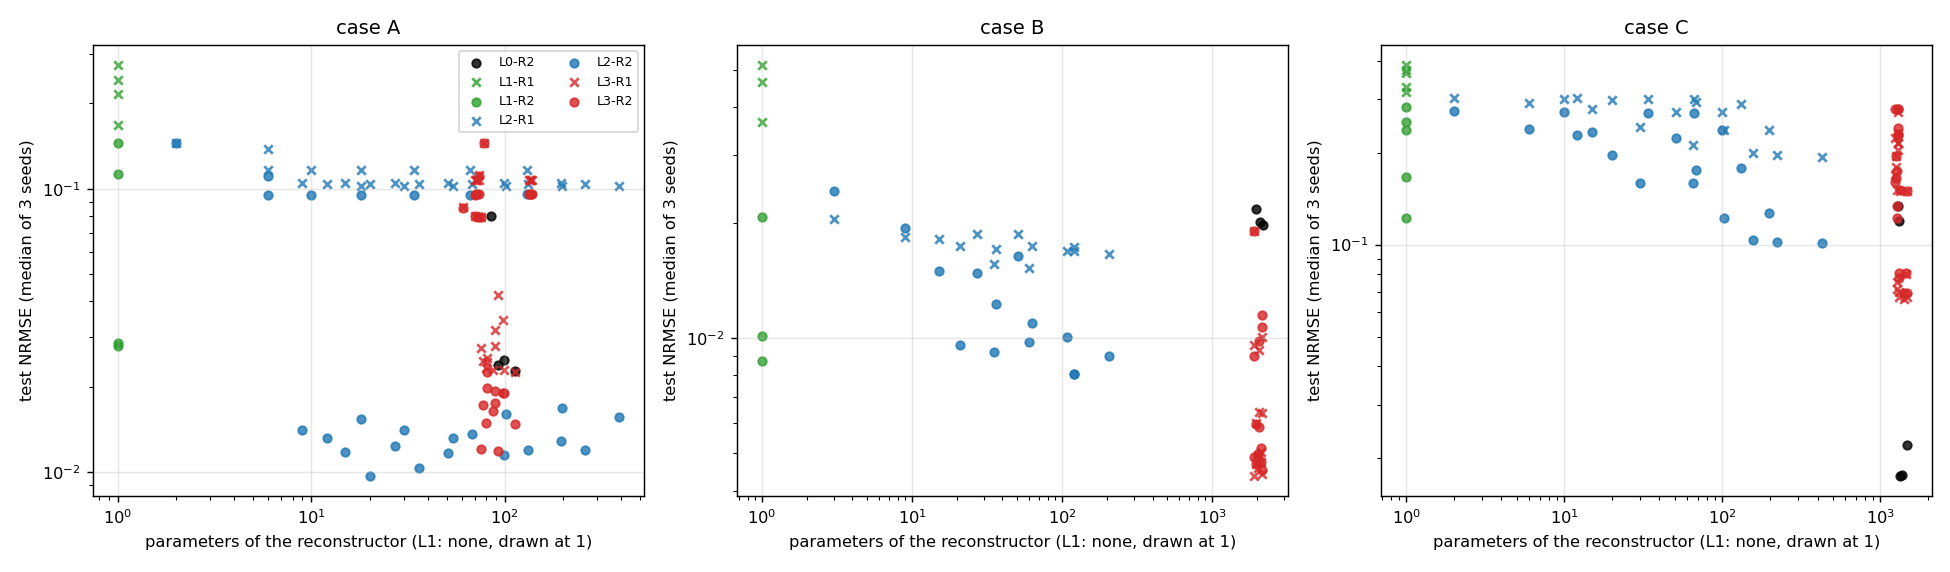
\includegraphics[width=0.90\textwidth,height=0.215\textheight,keepaspectratio]{fig5_pareto.png}
  \caption{Test NRMSE (median of 3 seeds) against reconstructor parameter count $P_{\mathrm{rec}}$ across all configurations of the \texttt{RQ2} sweeps in Cases~A, B, and~C (circles: end-to-end Regime~R2; crosses: frozen-latent Regime~R1; $\mathrm{L1}$ has $P_{\mathrm{rec}}=0$ and is plotted at $1$).}
  \label{fig:rq2_fig5}
\end{figure}

Figure~\ref{fig:rq2_fig3} confirms Proposition~\ref{prop:rec_rank_bound} across every single configuration of the study: the affine modal decoder $\mathrm{L2}$-R2 (blue curve) \textbf{never crosses below the black dashed rank floor $\varepsilon_{\mathrm{rank}}(r)$} (sitting directly on it at $d_s=1$ in Case~A, $0.566$ vs.\ $0.565$, and remaining above it everywhere in Cases~B and~C). By contrast, the nonlinear decoders breaks through the linear rank floor whenever $d_s$ is small: $\mathrm{L3}$-R2 goes below $\varepsilon_{\mathrm{rank}}(r)$ at $d_s=1$ in Case~A ($0.474$ vs.\ $0.565$), at $d_s=1$ in Case~B ($0.098$ vs.\ $0.156$), and at every $d_s \le 5$ in Case~C ($0.352$ vs.\ $0.426$ at $d_s=3$; $0.224$ vs.\ $0.299$ at $d_s=5$), while $\mathrm{L0}$ breaks the rank floor by a factor of $8.5\times$ in Case~C at $d_s=3$ ($0.050$ vs.\ $0.426$).

\subsection{Spectral Probing of the Trained \texorpdfstring{$\mathrm{L0}$}{L0} Decoder, Linear Invariants, and the Initial-State Handicap}
\label{sec:rq2_spectral_probing}

To understand how the trained implicit MLP $\NNrec(\mathbf{z},\mathbf{x})$ behaves internally on the states it visits, we project its test-set output $\hat{y}_{\mathrm{L0}}(\cdot,t) - \bar{y}$ onto the orthonormal basis $\{\varphi_k\}$ to extract its modal coefficients $\hat{c}_k^{\mathrm{L0}}(t) = \ip{\hat{y}_{\mathrm{L0}}(\cdot,t) - \bar{y}}{\varphi_k}$, and compute two diagnostic quantities defined in the protocol:
\begin{enumerate}[leftmargin=2em]
  \item The \textbf{linearizability index} $R^2_{\mathrm{lin}}(K)$, defined as the coefficient of determination of the best affine least-squares fit $\hat{\mathbf{c}}_{1:K}^{\mathrm{L0}}(t) \approx W\mathbf{z}(t) + \mathbf{b}$ over all test trajectories and time steps:
  \begin{equation}
    R^2_{\mathrm{lin}}(K) = 1 - \frac{\sum_{s,i} \norm{\hat{\mathbf{c}}_{1:K}^{\mathrm{L0}}(t_i) - \big(W\mathbf{z}^{(s)}(t_i) + \mathbf{b}\big)}_2^2}{\sum_{s,i} \norm{\hat{\mathbf{c}}_{1:K}^{\mathrm{L0}}(t_i) - \overline{\hat{\mathbf{c}}}_{1:K}^{\mathrm{L0}}}_2^2}.
    \label{eq:R2_lin}
  \end{equation}
  \item The \textbf{effective spectral width} $K_{99}$, defined at each test snapshot as the smallest mode count $K \le 65$ holding at least $99\%$ of the modal energy $\sum_{k=1}^{65} |\hat{c}_k(t)|^2$.
\end{enumerate}

\begin{figure}[!htbp]
  \centering
  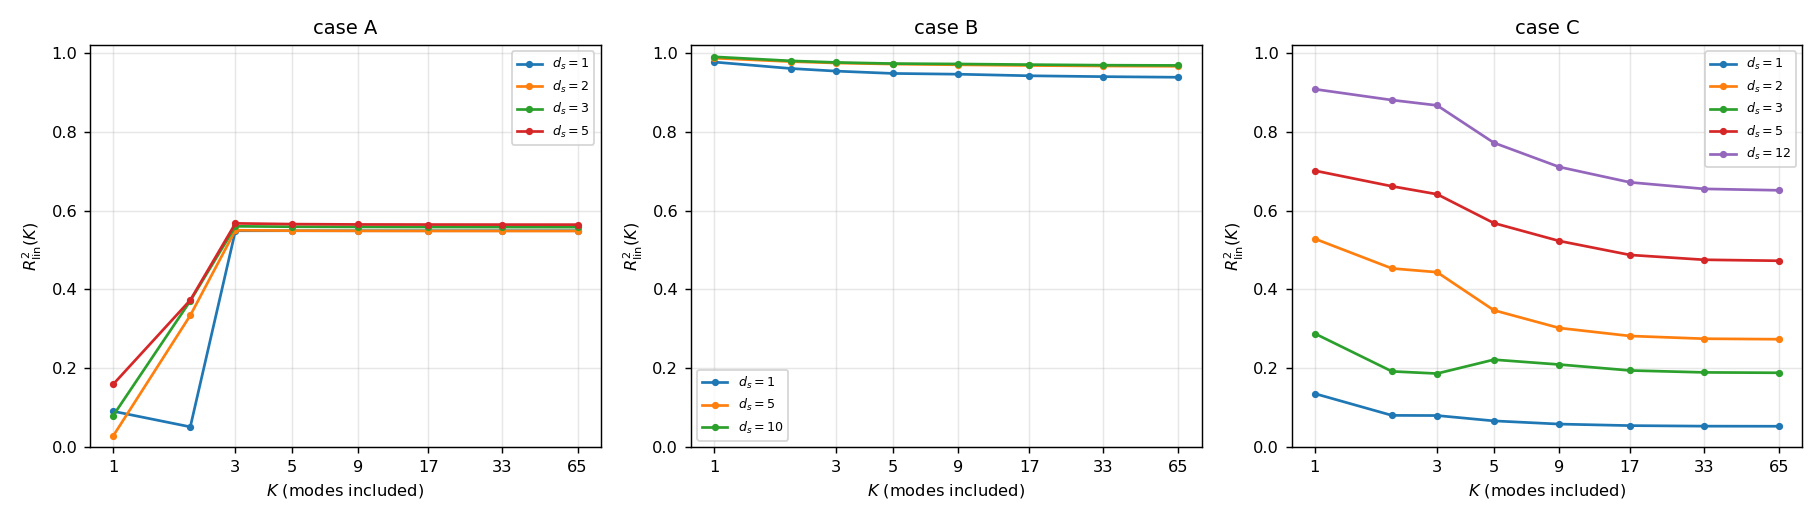
\includegraphics[width=0.90\textwidth,height=0.215\textheight,keepaspectratio]{fig4_L0_linearity.png}
  \caption{Linearizability index $R^2_{\mathrm{lin}}(K)$ of the trained $\mathrm{L0}$ reconstructor~\eqref{eq:R2_lin} against the number of included modes $K$ across latent dimensions $d_s$ (median of 3 seeds) for Case~A (left), Case~B (centre), and Case~C (right).}
  \label{fig:rq2_fig4}
\end{figure}

\begin{figure}[!htbp]
  \centering
  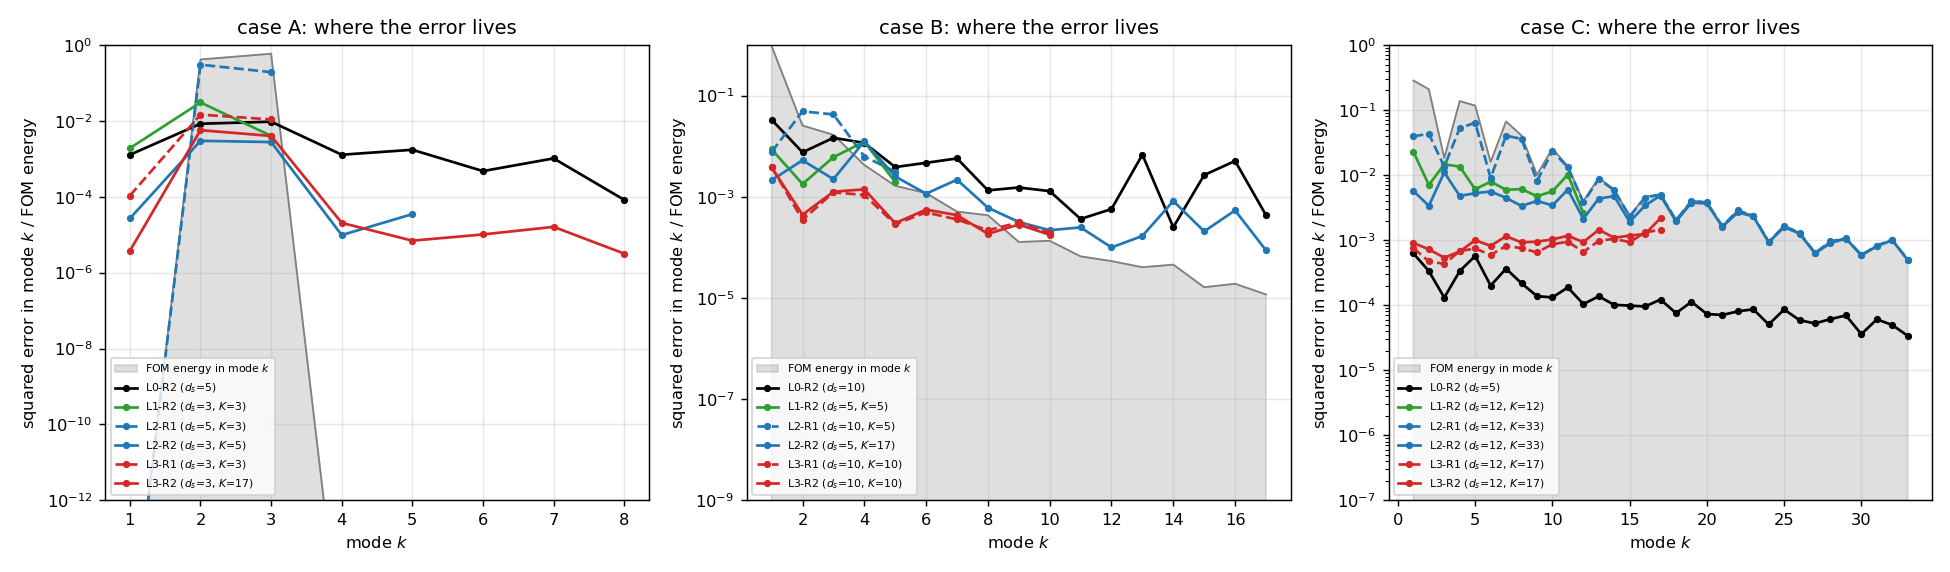
\includegraphics[width=0.90\textwidth,height=0.215\textheight,keepaspectratio]{fig6_modes.png}
  \caption{Per-mode coefficient error spectra $\norm{\hat{c}_k - c_k}_2$ (and true modal energy $\norm{c_k}_2$, black) across mode index $k$ at the reference latent size of each case in \texttt{RQ2}. Notice the spurious high-frequency spectral tail of $\mathrm{L0}$ for $k \ge 4$ in Case~A and $k \ge 10$ in Case~B.}
  \label{fig:rq2_fig6}
\end{figure}

Figures~\ref{fig:rq2_fig4} and~\ref{fig:rq2_fig6} reveal three deep structural properties of implicit MLP decoders versus modal expansions:
\begin{itemize}[leftmargin=2em]
  \item \textbf{Spurious high-wavenumber tails in $\mathrm{L0}$ and denoising via modal projection:} In Case~B, the true velocity field has a narrow spectral width of $K_{99} = 4$ POD modes (interquartile range $[2,6]$), and $\mathrm{L0}$ is almost perfectly affine in its inputs on the visited states ($R^2_{\mathrm{lin}}(K) \in [0.94, 0.99]$, Figure~\ref{fig:rq2_fig4} centre). Yet $\mathrm{L0}$'s output exhibits a massive spurious high-frequency tail with \textbf{$K_{99} = 42$ modes} (Figure~\ref{fig:rq2_fig6} centre)! Because spatial differentiation multiplies mode $k$ by its characteristic wavenumber, this spurious tail inflates $\mathrm{L0}$'s relative vorticity error in \texttt{RQ2} to $0.887$. Simply projecting $\mathrm{L0}$'s predicted velocity field onto the first $K=3$ POD modes (dash-dotted black curve in Figure~\ref{fig:rq2_fig2} centre) \textbf{reduces $\mathrm{L0}$'s test NRMSE by $40\%$} (from $1.97\cdot 10^{-2}$ to $1.19\cdot 10^{-2}$) and cuts its vorticity error from $0.887$ to $0.268$! Similarly, projecting $\mathrm{L0}$ onto $K=3$ Fourier modes in Case~A lowers its NRMSE by $10\%$ ($2.49\cdot 10^{-2} \to 2.23\cdot 10^{-2}$). Conversely, in Case~C both the FOM and $\mathrm{L0}$ have $K_{99} = 25$ modes, and projecting $\mathrm{L0}$ onto $K \le 33$ modes destroys the sharp front profile ($2.21\cdot 10^{-2} \to 3.20\cdot 10^{-2}$ at $K=33$ and $5.82\cdot 10^{-2}$ at $K=17$).
  \item \textbf{Inheritance of linear physical invariants (discrete incompressibility):} Because every vector POD mode $\boldsymbol{\varphi}_k(\mathbf{x})$ in Case~B is a linear combination of divergence-free FOM velocity snapshots, any modal expansion $\hat{\mathbf{v}} = \bar{\mathbf{v}} + \sum_{k=1}^K c_k(t)\boldsymbol{\varphi}_k(\mathbf{x})$ automatically inherits the discrete divergence level of the FOM grid: measuring $\norm{\nabla\cdot\mathbf{v}}_2 / \norm{\nabla\mathbf{v}}_2$ by central differences on the $100\times 100$ grid yields \textbf{$0.0696$ for the FOM and $0.0696$ ($[0.0693, 0.0699]$) for $\mathrm{L3}$-R1}, whereas the unconstrained pointwise MLP $\mathrm{L0}$ gives $0.270$ ($[0.210, 0.331]$, nearly $4\times$ higher divergence in \texttt{RQ2}, and still $1.9\times$ higher even after $10{,}000$ BFGS iterations in \texttt{RQ2-bis}).
  \item \textbf{The initial-state handicap of $\mathrm{L1}$:} Because all modal variants add the non-zero time-averaged training field $\bar{y}(\mathbf{x})$ ($\mathrm{rms}(\bar{y})/\mathrm{rms}(y) = 0.520, 0.175, 0.481$ in Cases~A, B, C) while the latent ODE starts at $\mathbf{s}(0) = \mathbf{0}$, the parameter-free identity decoder $\mathrm{L1}$ ($\hat{y}(\cdot,0) = \bar{y} + \sum_k 0\cdot\varphi_k = \bar{y}$) is forced to predict the mean field instead of the zero rest state at $t = 0$! By contrast, $\mathrm{L2}$ and $\mathrm{L3}$ use their trainable bias $\mathbf{b}$ or $g_\theta(\mathbf{0})$ to cancel $P_K\bar{y}$ at $t=0$ (reducing the $t=0$ relative error from $0.520$ to $0.011$ in Case~A and from $0.175$ to $0.004$ in Case~B). In Case~A, this initial-state mismatch accounts for \textbf{$53.7\%$ of the total squared error of $\mathrm{L1}$-R2} over the entire 201-step horizon taking place in just the first 20 time steps!
\end{itemize}

\section{Part II: Computational Scalability under Full Quasi-Newton Optimization (\texttt{RQ2-bis})}
\label{sec:rq2bis}

While \texttt{RQ2} established which reconstructor architectures can represent each PDE family at fixed dynamics capacity and a short 200 Adam + 500 BFGS budget, two fundamental questions remained open:
\begin{enumerate}[leftmargin=2em]
  \item In Case~B, where the 17-mode POD floor is $\NRMSE = 3.46\cdot 10^{-4}$ ($57\times$ below \texttt{RQ2}'s $\mathrm{L0}$ and $23\times$ below \texttt{RQ2}'s $\mathrm{L2}$), was the accuracy of end-to-end training bottlenecked by the tiny canonical dynamics network ($7\text{--}7\text{--}d_s$, having only $85$--$220$ parameters) or by the $500$-iteration BFGS cap?
  \item Across both smooth vortex flows (Case~B) and sharp travelling fronts (Case~C), how does the test error $\NRMSE(P_{\mathrm{dyn}}, L, n, \text{iterations})$ scale when the dynamics network width $w$, depth $L$, latent dimension $n$, and quasi-Newton iteration budget are scaled up to $10{,}000$ BFGS iterations?
\end{enumerate}

\subsection{Experimental Design and the CINECA Leonardo HPC Campaign}

To trace the complete surface $\mathrm{error}(P, \text{iterations})$ without confounding from a first-order learning-rate schedule or an arbitrary Adam-to-BFGS switch point, \texttt{RQ2-bis} removes the Adam warm-up (\texttt{epochs\_adam = 0}) and optimizes all models from Glorot initialization using pure \texttt{scipy} BFGS (\texttt{method='BFGS'}, \texttt{gtol=1e-100}, \texttt{maxiter=10000}). Because a deterministic quasi-Newton trajectory has no learning-rate schedule---its step at iteration $k$ depends exclusively on the current gradient and the inverse-Hessian approximation accumulated over steps $0,\dots,k-1$---a single run of $I_{\max} = 10{,}000$ iterations equipped with a passive observation hook (\texttt{callback\_extra}) at the nine logarithmic checkpoints
\begin{equation}
  k \in \{25,\, 50,\, 100,\, 200,\, 500,\, 1000,\, 2000,\, 5000,\, 10000\}
  \label{eq:checkpoints}
\end{equation}
is mathematically identical to nine independent training runs stopped at each $k$. The time spent evaluating validation and full-grid test metrics inside the checkpoint hook (\texttt{ck\_time}) is explicitly measured and subtracted from both \texttt{train\_time\_s} and the cumulative trajectory time \texttt{time\_s} in \texttt{curves.csv}.

In each benchmark (Case~B and Case~C), we run two end-to-end ($\mathrm{R2}$) reconstructor arms across 21 configurations $\times$ 3 seeds $= 63$ runs per case (126 runs in total):
\begin{itemize}[leftmargin=2em]
  \item \textbf{Main Arm ($\mathrm{L0}$, Stages 0--2, 10 configs $\times$ 3 seeds $= 30$ runs/case):} The original pointwise MLP reconstructor ($24^4\to 2$ with cubic link in Case~B; $17^5\to 1$ in Case~C), sweeping:
  \begin{enumerate}[label=(\alph*)]
    \item \emph{Dynamics hidden width} $w \in \{w^*/4, w^*/2, w^*, 2w^*, 4w^*\}$ at canonical depth $L^*$ and latent size $n^*$, namely $w \in \{2, 4, 7, 14, 28\}$ at $(L^*=2, n^*=1)$ in Case~B ($P_{\mathrm{dyn}} \in \{15, 37, 85, 267, 925\}$) and $w \in \{2, 4, 8, 16, 32\}$ at $(L^*=1, n^*=12)$ in Case~C ($P_{\mathrm{dyn}} \in \{66, 120, 228, 444, 876\}$);
    \item \emph{Dynamics hidden depth} $L \in \{1, 2, 3\}$ at canonical $(w^*, n^*)$;
    \item \emph{Latent dimension} $n \in \{1, 2, 5, 10\}$ in Case~B and $n \in \{3, 6, 12, 24\}$ in Case~C at canonical $(w^*, L^*)$.
  \end{enumerate}
  \item \textbf{Linear Reconstructor Arm ($\mathrm{L2}$, Stage 7, 11 configs $\times$ 3 seeds $= 33$ runs/case):} The strictly linear modal synthesis $\bar{y}(\mathbf{x}) + \sum_{k=1}^K (W\mathbf{z}+\mathbf{b})_k \varphi_k(\mathbf{x})$ on the vector POD basis (Case~B) or trapezoidal-QR Legendre basis (Case~C), sweeping:
  \begin{enumerate}[label=(\alph*)]
    \item \emph{Latent dimension} $n \in \{1, 2, 5, 10\}$ (Case~B) and $n \in \{3, 6, 12, 24\}$ (Case~C) at $K_{\mathrm{L2}} = 65$ and canonical $(w^*, L^*)$;
    \item \emph{Dynamics hidden width} $w \in \{2, 4, 7, 14, 28\}$ at $(n_{\mathrm{L2}}=10, K=65, L^*=2)$ in Case~B ($P_{\mathrm{dyn}} \in \{60, 118, 220, 528, 1438\}$) and $w \in \{2, 4, 8, 16, 32\}$ at $(n_{\mathrm{L2}}=12, K=65, L^*=1)$ in Case~C ($P_{\mathrm{dyn}} \in \{66, 120, 228, 444, 876\}$);
    \item \emph{Basis truncation size} $K \in \{5, 17, 33, 65\}$ at $(w^*, L^*, n_{\mathrm{L2}})$.
  \end{enumerate}
\end{itemize}

\paragraph{Two-Pass Hardware Execution on CINECA Leonardo.}
An initial $1{,}000$-iteration pilot campaign of all 126 runs on an Apple M5 Pro workstation (18 CPU cores, 48~GB unified memory, preserved in \texttt{results\_1000iters/}) revealed that at iteration $1{,}000$ the test NRMSE was still dropping by $25\%$ to $49\%$ over the last 500 iterations across nearly all $\mathrm{L0}$ configurations. We therefore raised the budget tenfold to \textbf{$I_{\max} = 10{,}000$ BFGS iterations} (matching the original paper's full Case~B BFGS budget and doubling its Case~C budget) and executed the production campaign on the \textbf{Data Centric General Purpose (\texttt{dcgp\_usr\_prod}) partition of the CINECA Leonardo supercomputer} (dual-socket Intel Xeon Platinum 8480+ ``Sapphire Rapids'' compute nodes, $2 \times 56 = 112$ physical CPU cores per node, Linux 4.18, Python 3.11.7, TensorFlow 2.13.1 in IEEE-754 \texttt{float64} precision).

To prevent multi-job node contention from contaminating wall-clock measurements, we enforced a strict two-pass protocol:
\begin{enumerate}[leftmargin=2em]
  \item \textbf{Pass A (Accuracy Sweeps):} Each case was partitioned across four Slurm array shards (\texttt{--array=0-3}, 56 cores per shard) via \texttt{RQ2BIS\_SHARD=i/4}, recording all weights, predictions, checkpoint trajectories, function/gradient evaluation counts $n_{\mathrm{fev}}$, and shared-node wall-times $T_{\mathrm{Pass\,A}}$, then merged via \texttt{cluster/merge\_results.py}.
  \item \textbf{Pass T (Exclusive-Node Timing and Thread Scaling, Stage 5):} Following Pass~A, we allocated one \textbf{exclusive} 112-core Leonardo compute node per case (\texttt{--exclusive}, node \texttt{lrdn4887} for Case~B, Slurm job \texttt{60616414}; node \texttt{lrdn4960} for Case~C, Slurm job \texttt{60616416}). Because TensorFlow locks its thread pool upon initialisation, \texttt{timing\_worker.py} spawns a fresh subprocess for each thread count $p \in \{1, 2, 4, 8, 16, 32, 64, 112\}$ (setting \texttt{OMP\_NUM\_THREADS = MKL\_NUM\_THREADS = OPENBLAS\_NUM\_THREADS = p} and TensorFlow's intra/inter-op threads to $p$ prior to import), loads the exact trained weights from \texttt{results/weights/}, performs a warm-up evaluation, and measures the median over 3 repeats of the mean of 20 joint loss-and-gradient evaluations ($s_{\mathrm{eval}}$). At the optimal operating point $p^* = 16$ threads, all 21 configurations of the case are timed in randomized order (\texttt{RandomState(0).permutation}), with the first configuration repeated at the end to verify absence of thermal or cluster throttling ($1.3\%$ drift in Case~B; $7.6\%$ in Case~C, both well within the $10\%$ protocol threshold). The uncontaminated \textbf{Pass-T training wall-time} of any run is then $T_{\mathrm{Pass\,T}} = n_{\mathrm{fev}} \times s_{\mathrm{eval}}$.
\end{enumerate}

\subsection{Case B Scalability Results: \texorpdfstring{$\mathrm{L0}$}{L0} Plateau vs.\ \texorpdfstring{$\mathrm{L2}$}{L2} Power-Law Scaling}

Table~\ref{tab:rq2bis_caseB} reports the complete results of all 21 configurations in Case~B at the $10{,}000$-iteration BFGS budget, and Figure~\ref{fig:rq2bis_fig1} (left column) shows the resulting capacity scaling curves against $P_{\mathrm{dyn}}$ and $P_{\mathrm{total}}$.

\begin{figure}[!htbp]
  \centering
  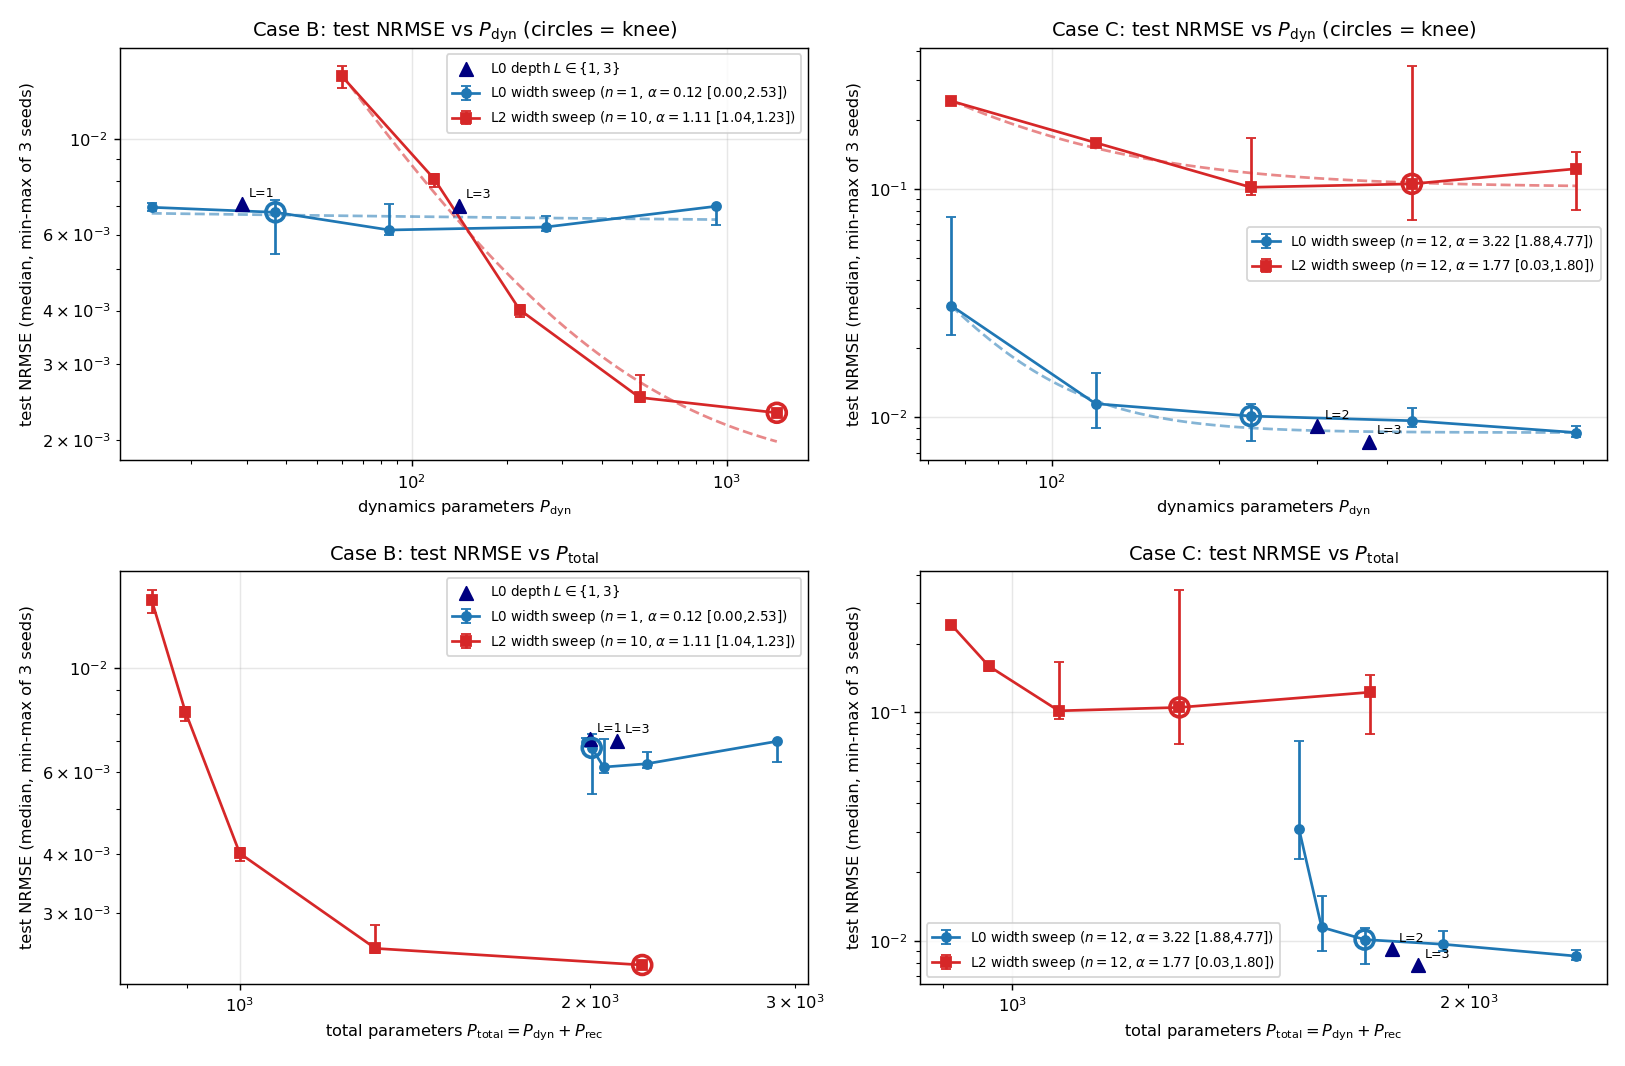
\includegraphics[width=0.90\textwidth,height=0.215\textheight,keepaspectratio]{fig1_capacity_laws.png}
  \caption{Stage~1 capacity scaling at the $10{,}000$-iteration BFGS budget on CINECA Leonardo: test NRMSE (median and min--max range over 3 seeds) against dynamics parameters $P_{\mathrm{dyn}}$ (\textbf{top row}, with fitted power laws $E(P_{\mathrm{dyn}}) = E_\infty + a\,P_{\mathrm{dyn}}^{-\alpha}$ dashed and validation-selected knees circled) and against total parameters $P_{\mathrm{total}} = P_{\mathrm{dyn}} + P_{\mathrm{rec}}$ (\textbf{bottom row}), for Case~B (\textbf{left}) and Case~C (\textbf{right}).}
  \label{fig:rq2bis_fig1}
\end{figure}

\begin{table}[!htbp]
\centering
\caption{Case B (\texttt{2D-Stokes}): all 21 configurations at the $10{,}000$-iteration BFGS budget on CINECA Leonardo (median and $[\min,\max]$ over 3 seeds). Here \texttt{st} is the number of early-stopped seeds out of 3, $s_{\mathrm{eval}}$ is the exclusive-node Pass-T evaluation time at 16 threads, $T_{\mathrm{Pass\,T}} = n_{\mathrm{fev}} s_{\mathrm{eval}}$, and $\eta = \varepsilon_{\mathrm{total}}/\varepsilon_{\mathrm{proj}}$. Bold rows mark the validation-selected best configuration of each arm.}
\label{tab:rq2bis_caseB}
\scriptsize
\setlength{\tabcolsep}{3.5pt}\resizebox{\textwidth}{!}{%

\begin{tabular}{@{}lrrrrrrrrrrrrrrlrr@{}}
\toprule
\textbf{Arm} & $K$ & $w$ & $L$ & $n$ & \textbf{st} & $P_{\mathrm{dyn}}$ & $P_{\mathrm{rec}}$ & $P_{\mathrm{tot}}$ & $\min\text{it}$ & $n_{\mathrm{fev}}$ & $s_{\mathrm{eval}}$[s] & $T_{\mathrm{PassT}}$[s] & $T_{\mathrm{PassA}}$[s] & \textbf{Valid} & \textbf{Test NRMSE $[\min,\max]$} & \textbf{Dir.} & \textbf{Vort.} \\
\midrule
L0 & $0$ & $2$ & $2$ & $1$ & $0$ & $15$ & $1970$ & $1985$ & $10000$ & $10042$ & $0.308$ & $3090$ & $4620$ & $5.84\cdot 10^{-3}$ & $6.94\cdot 10^{-3}$ $[6.82, 7.10]\cdot 10^{-3}$ & $0.0214$ & $0.389$ \\
L0 & $0$ & $4$ & $2$ & $1$ & $0$ & $37$ & $1970$ & $2007$ & $10000$ & $10042$ & $0.315$ & $3160$ & $4840$ & $5.65\cdot 10^{-3}$ & $6.76\cdot 10^{-3}$ $[5.40, 7.23]\cdot 10^{-3}$ & $0.0208$ & $0.358$ \\
L0 & $0$ & $7$ & $1$ & $1$ & $0$ & $29$ & $1970$ & $1999$ & $10000$ & $10044$ & $0.312$ & $3130$ & $4900$ & $5.92\cdot 10^{-3}$ & $7.06\cdot 10^{-3}$ $[6.86, 7.44]\cdot 10^{-3}$ & $0.0219$ & $0.429$ \\
L0 & $0$ & $7$ & $2$ & $1$ & $0$ & $85$ & $1970$ & $2055$ & $10000$ & $10050$ & $0.313$ & $3140$ & $4910$ & $5.27\cdot 10^{-3}$ & $6.15\cdot 10^{-3}$ $[5.98, 7.07]\cdot 10^{-3}$ & $0.0209$ & $0.312$ \\
L0 & $0$ & $7$ & $2$ & $2$ & $0$ & $100$ & $1994$ & $2094$ & $10000$ & $10041$ & $0.316$ & $3170$ & $4840$ & $5.56\cdot 10^{-3}$ & $6.61\cdot 10^{-3}$ $[5.96, 6.76]\cdot 10^{-3}$ & $0.0148$ & $0.408$ \\
\textbf{L0} & $\mathbf{0}$ & $\mathbf{7}$ & $\mathbf{2}$ & $\mathbf{5}$ & $\mathbf{0}$ & $\mathbf{145}$ & $\mathbf{2066}$ & $\mathbf{2211}$ & $\mathbf{10000}$ & $\mathbf{10035}$ & $\mathbf{0.354}$ & $\mathbf{3560}$ & $\mathbf{5660}$ & $\mathbf{5.13\cdot 10^{-3}}$ & $\mathbf{5.86\cdot 10^{-3}}$ $[5.13, 6.69]\cdot 10^{-3}$ & $\mathbf{0.0130}$ & $\mathbf{0.348}$ \\
L0 & $0$ & $7$ & $2$ & $10$ & $0$ & $220$ & $2186$ & $2406$ & $10000$ & $10034$ & $0.364$ & $3650$ & $5820$ & $5.58\cdot 10^{-3}$ & $6.37\cdot 10^{-3}$ $[6.06, 6.56]\cdot 10^{-3}$ & $0.0163$ & $0.424$ \\
L0 & $0$ & $7$ & $3$ & $1$ & $0$ & $141$ & $1970$ & $2111$ & $10000$ & $10043$ & $0.313$ & $3150$ & $5170$ & $5.88\cdot 10^{-3}$ & $7.00\cdot 10^{-3}$ $[6.87, 7.11]\cdot 10^{-3}$ & $0.0210$ & $0.404$ \\
L0 & $0$ & $14$ & $2$ & $1$ & $0$ & $267$ & $1970$ & $2237$ & $10000$ & $10046$ & $0.320$ & $3210$ & $5140$ & $5.32\cdot 10^{-3}$ & $6.25\cdot 10^{-3}$ $[6.13, 6.62]\cdot 10^{-3}$ & $0.0200$ & $0.348$ \\
L0 & $0$ & $28$ & $2$ & $1$ & $0$ & $925$ & $1970$ & $2895$ & $10000$ & $10037$ & $0.321$ & $3230$ & $7040$ & $5.85\cdot 10^{-3}$ & $6.98\cdot 10^{-3}$ $[6.31, 6.98]\cdot 10^{-3}$ & $0.0214$ & $0.391$ \\
\midrule
L2 & $5$ & $7$ & $2$ & $10$ & $1$ & $220$ & $60$ & $280$ & $7143$ & $10390$ & $0.0251$ & $261$ & $599$ & $5.01\cdot 10^{-3}$ & $6.26\cdot 10^{-3}$ $[5.62, 6.73]\cdot 10^{-3}$ & $0.0321$ & $0.163$ \\
L2 & $17$ & $7$ & $2$ & $10$ & $0$ & $220$ & $204$ & $424$ & $10000$ & $10218$ & $0.0340$ & $347$ & $724$ & $4.56\cdot 10^{-3}$ & $4.68\cdot 10^{-3}$ $[4.61, 6.10]\cdot 10^{-3}$ & $0.0168$ & $0.156$ \\
L2 & $33$ & $7$ & $2$ & $10$ & $0$ & $220$ & $396$ & $616$ & $10000$ & $10134$ & $0.0421$ & $427$ & $1100$ & $3.83\cdot 10^{-3}$ & $4.18\cdot 10^{-3}$ $[3.95, 4.22]\cdot 10^{-3}$ & $0.0128$ & $0.127$ \\
L2 & $65$ & $2$ & $2$ & $10$ & $3$ & $60$ & $780$ & $840$ & $2905$ & $3042$ & $0.0610$ & $185$ & $381$ & $1.25\cdot 10^{-2}$ & $1.40\cdot 10^{-2}$ $[1.31, 1.47]\cdot 10^{-2}$ & $0.0695$ & $0.422$ \\
L2 & $65$ & $4$ & $2$ & $10$ & $1$ & $118$ & $780$ & $898$ & $7195$ & $10207$ & $0.0618$ & $631$ & $1300$ & $7.86\cdot 10^{-3}$ & $8.07\cdot 10^{-3}$ $[7.73, 8.27]\cdot 10^{-3}$ & $0.0272$ & $0.206$ \\
L2 & $65$ & $7$ & $2$ & $1$ & $0$ & $85$ & $195$ & $280$ & $10000$ & $10592$ & $0.0631$ & $668$ & $1070$ & $1.39\cdot 10^{-2}$ & $1.68\cdot 10^{-2}$ $[1.54, 1.68]\cdot 10^{-2}$ & $0.0692$ & $0.452$ \\
L2 & $65$ & $7$ & $2$ & $2$ & $0$ & $100$ & $260$ & $360$ & $10000$ & $10386$ & $0.0631$ & $655$ & $1100$ & $8.48\cdot 10^{-3}$ & $9.61\cdot 10^{-3}$ $[9.55, 9.78]\cdot 10^{-3}$ & $0.0228$ & $0.196$ \\
L2 & $65$ & $7$ & $2$ & $5$ & $0$ & $145$ & $455$ & $600$ & $10000$ & $10180$ & $0.0630$ & $641$ & $1300$ & $4.06\cdot 10^{-3}$ & $4.34\cdot 10^{-3}$ $[4.24, 4.44]\cdot 10^{-3}$ & $0.0053$ & $0.138$ \\
L2 & $65$ & $7$ & $2$ & $10$ & $0$ & $220$ & $780$ & $1000$ & $10000$ & $10113$ & $0.0635$ & $642$ & $1390$ & $3.73\cdot 10^{-3}$ & $4.02\cdot 10^{-3}$ $[3.88, 4.12]\cdot 10^{-3}$ & $0.0119$ & $0.126$ \\
L2 & $65$ & $14$ & $2$ & $10$ & $0$ & $528$ & $780$ & $1308$ & $10000$ & $10061$ & $0.0654$ & $658$ & $1610$ & $2.71\cdot 10^{-3}$ & $2.52\cdot 10^{-3}$ $[2.46, 2.83]\cdot 10^{-3}$ & $0.0019$ & $0.071$ \\
\textbf{L2} & $\mathbf{65}$ & $\mathbf{28}$ & $\mathbf{2}$ & $\mathbf{10}$ & $\mathbf{0}$ & $\mathbf{1438}$ & $\mathbf{780}$ & $\mathbf{2218}$ & $\mathbf{10000}$ & $\mathbf{10076}$ & $\mathbf{0.0738}$ & $\mathbf{744}$ & $\mathbf{3090}$ & $\mathbf{2.07\cdot 10^{-3}}$ & $\mathbf{2.32\cdot 10^{-3}}$ $[2.32, 2.36]\cdot 10^{-3}$ & $\mathbf{0.0014}$ & $\mathbf{0.067}$ \\
\bottomrule
\end{tabular}
}
\end{table}

Table~\ref{tab:rq2bis_caseB} and Figure~\ref{fig:rq2bis_fig1} (left) reveal a striking dichotomy between the nonlinear reconstructor $\mathrm{L0}$ and the linear POD reconstructor $\mathrm{L2}$:
\begin{enumerate}[leftmargin=2em]
  \item \textbf{Why scaling $\NNdyn$ in Case B $\mathrm{L0}$ at $n^*=1$ produces a flat line:} Across the entire $\mathrm{L0}$ width sweep $w \in \{2, 4, 7, 14, 28\}$ ($P_{\mathrm{dyn}}$ increasing by $62\times$, from $15$ to $925$), the median test NRMSE stays trapped inside the narrow band $[6.15\cdot 10^{-3}, 6.98\cdot 10^{-3}]$. The two-point log-log slopes $\mathrm{d}\log E / \mathrm{d}\log P_{\mathrm{dyn}}$ are $[-0.030, -0.113, +0.014, +0.089]$, and the power-law fit gives $\alpha = 0.118$ with a 95\% bootstrap confidence interval $[0.000, 2.525]$ reaching zero, falsifying Hypothesis~H1 for Case~B $\mathrm{L0}$. Varying depth ($L \in \{1,2,3\}$: $7.06, 6.15, 7.00\cdot 10^{-3}$) or increasing the latent dimension at canonical dynamics width ($n \in \{1,2,5,10\}$: $6.15, 6.61, 5.86, 6.37\cdot 10^{-3}$) changes the error by at most $5\%$. At $n^*=1$, a single scalar latent state $s(t)$ cannot encode more than one degree of freedom of the flow history regardless of how wide $\NNdyn$ is, and when $n$ is raised to $5$ or $10$, the joint quasi-Newton optimization of $\NNdyn$ and the 4-layer pointwise MLP $\NNrec$ ($P_{\mathrm{rec}} \approx 2000$) is bottlenecked by the ill-conditioned non-convex landscape of the spatial MLP and by the narrow $w^*=7$ dynamics layer.
  \item \textbf{Replacing $\mathrm{L0}$ with $\mathrm{L2}$ ($n=10, K=65$) unlocks a textbook power law ($\alpha = 1.11$) and beats $\mathrm{L0}$ by $2.5\times$ in error:} Once the pointwise MLP is replaced by the linear POD basis $\mathrm{L2}$ and $n=10$ latent states are provided, widening $\NNdyn$ through $w \in \{2, 4, 7, 14, 28\}$ ($P_{\mathrm{dyn}} \in \{60, 118, 220, 528, 1438\}$) drives the median test NRMSE down monotonically across every single step:
  \begin{equation}
    1.40\cdot 10^{-2} \;\xrightarrow{w=4}\; 8.07\cdot 10^{-3} \;\xrightarrow{w=7}\; 4.02\cdot 10^{-3} \;\xrightarrow{w=14}\; 2.52\cdot 10^{-3} \;\xrightarrow{w=28}\; \mathbf{2.32\cdot 10^{-3}}.
    \label{eq:caseB_L2_progression}
  \end{equation}
  The power-law fit $E(P_{\mathrm{dyn}}) = E_\infty + a\,P_{\mathrm{dyn}}^{-\alpha}$ yields an asymptotic floor $E_\infty = 1.63\cdot 10^{-3}$ and exponent $\alpha = 1.113$ with a tight 95\% bootstrap CI of $[1.042, 1.226]$ (200/200 bootstrap refits converged), strongly supporting Hypothesis~H1. Notice how this resolves the puzzle left open by \texttt{RQ2}: in \texttt{RQ2} (500 BFGS epochs, $w^*=7$), $\mathrm{L2}$ stalled at $8.06\cdot 10^{-3}$ ($\eta = 26$); raising the BFGS budget to $10{,}000$ iterations halves the error at $w^*=7$ to $4.02\cdot 10^{-3}$, and widening $\NNdyn$ to $w=28$ (which lifts the dynamics rank bottleneck of Proposition~\ref{prop:dyn_rank_bound}) cuts it nearly in half again to \textbf{$2.32\cdot 10^{-3}$}!
  \item \textbf{Superior physical fidelity of $\mathrm{L2}$ in Case B (Figure~\ref{fig:rq2bis_fig8}):} Compared with the best $\mathrm{L0}$ configuration ($w=7, L=2, n=5$, $\NRMSE = 5.86\cdot 10^{-3}$), the best $\mathrm{L2}$ configuration ($K=65, w=28, L=2, n=10$, $\NRMSE = 2.32\cdot 10^{-3}$) reduces the velocity direction error by \textbf{$9.5\times$} ($0.00137$ vs.\ $0.0130$), reduces the relative vorticity error by \textbf{$5.2\times$} ($0.0669$ vs.\ $0.3484$), and preserves the exact discrete divergence floor of the FOM grid ($\norm{\nabla\cdot\mathbf{v}}/\norm{\nabla\mathbf{v}} = 0.0688$ vs.\ $0.0696$ for FOM, whereas $\mathrm{L0}$ has $0.1264$--$0.1330$).
\end{enumerate}

\begin{figure}[!htbp]
  \centering
  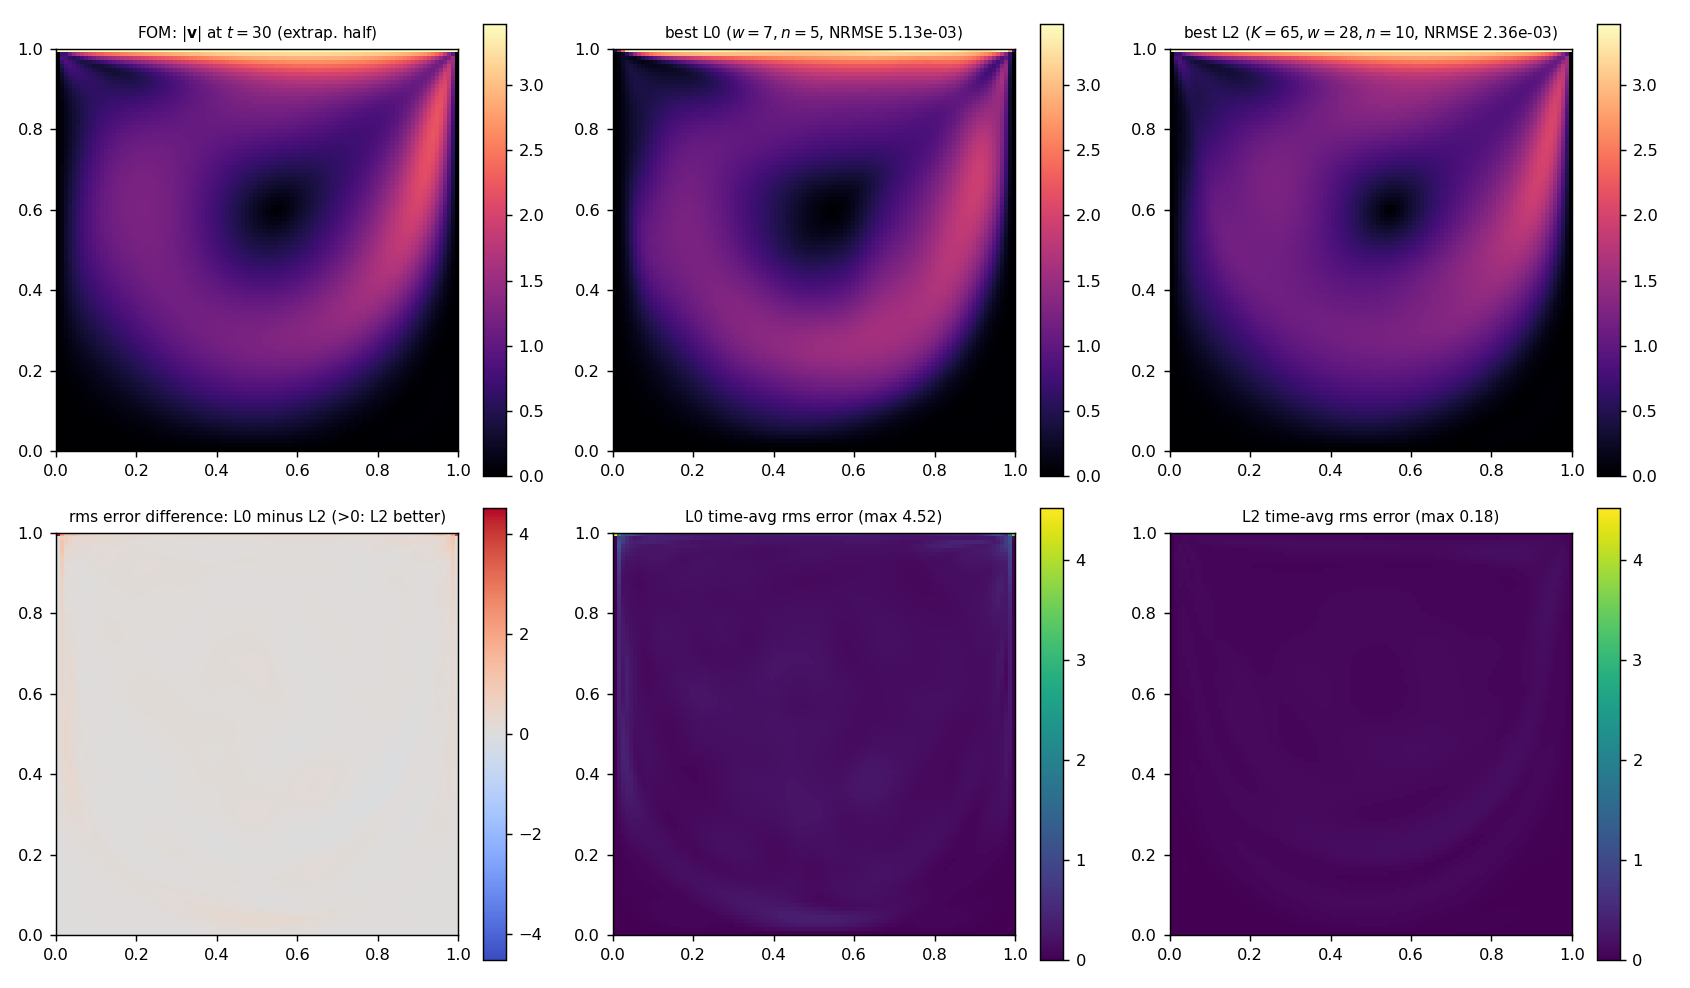
\includegraphics[width=0.90\textwidth,height=0.215\textheight,keepaspectratio]{fig8_B_fields_and_errors.png}
  \caption{Case B physical velocity fields and spatial error distribution at the $10{,}000$-iteration BFGS budget (test trajectory 0 at $t=30$, inside the time-extrapolation window $[20,40]$). \textbf{Top row:} velocity magnitude $\norm{\mathbf{v}}_2$ for the FOM ground truth (left), the best $\mathrm{L0}$ model ($w=7, L=2, n=5$, $\NRMSE = 5.86\cdot 10^{-3}$, centre), and the best $\mathrm{L2}$ model ($K=65, w=28, L=2, n=10$, $\NRMSE = 2.32\cdot 10^{-3}$, right). \textbf{Bottom row:} time-averaged pointwise rms error difference $\mathrm{err}_{\mathrm{L0}}(\mathbf{x}) - \mathrm{err}_{\mathrm{L2}}(\mathbf{x})$ (left, positive throughout the top-lid boundary layer and primary vortex core) and individual rms error maps of $\mathrm{L0}$ (centre) and $\mathrm{L2}$ (right) on a common colour scale.}
  \label{fig:rq2bis_fig8}
\end{figure}

\subsection{Case C Scalability Results: Steep \texorpdfstring{$\mathrm{L0}$}{L0} Capacity Law, Depth vs.\ Width, and Polynomial Overfitting of \texorpdfstring{$\mathrm{L2}$}{L2}}

Table~\ref{tab:rq2bis_caseC} reports all 21 configurations of Case~C at the $10{,}000$-iteration BFGS budget on CINECA Leonardo, and Figure~\ref{fig:rq2bis_fig9} compares the resulting space-time action-potential fields.

\begin{table}[!htbp]
\centering
\caption{Case C (\texttt{AP1D}): all 21 configurations at the $10{,}000$-iteration BFGS budget on CINECA Leonardo (median and $[\min,\max]$ over 3 seeds). Columns match Table~\ref{tab:rq2bis_caseB}, with Case~C's goal-oriented metrics: activation-time MAE (ms) and fraction of missed activations (\texttt{miss}).}
\label{tab:rq2bis_caseC}
\scriptsize
\setlength{\tabcolsep}{3.3pt}\resizebox{\textwidth}{!}{%

\begin{tabular}{@{}lrrrrrrrrrrrrrrlrr@{}}
\toprule
\textbf{Arm} & $K$ & $w$ & $L$ & $n$ & \textbf{st} & $P_{\mathrm{dyn}}$ & $P_{\mathrm{rec}}$ & $P_{\mathrm{tot}}$ & $\min\text{it}$ & $n_{\mathrm{fev}}$ & $s_{\mathrm{eval}}$[s] & $T_{\mathrm{PassT}}$[s] & $T_{\mathrm{PassA}}$[s] & \textbf{Valid} & \textbf{Test NRMSE $[\min,\max]$} & \textbf{MAE[ms]} & \textbf{miss} \\
\midrule
L0 & $0$ & $2$ & $1$ & $12$ & $0$ & $66$ & $1480$ & $1546$ & $10000$ & $10077$ & $0.266$ & $2680$ & $3700$ & $5.26\cdot 10^{-2}$ & $3.08\cdot 10^{-2}$ $[2.29, 7.51]\cdot 10^{-2}$ & $2.64$ & $0.001$ \\
L0 & $0$ & $4$ & $1$ & $12$ & $0$ & $120$ & $1480$ & $1600$ & $10000$ & $10042$ & $0.268$ & $2700$ & $3730$ & $9.58\cdot 10^{-3}$ & $1.15\cdot 10^{-2}$ $[8.99\cdot 10^{-3}, 1.56\cdot 10^{-2}]$ & $0.73$ & $0.000$ \\
L0 & $0$ & $8$ & $1$ & $3$ & $0$ & $75$ & $1327$ & $1402$ & $10000$ & $10035$ & $0.257$ & $2580$ & $3070$ & $1.40\cdot 10^{-2}$ & $2.22\cdot 10^{-2}$ $[1.06, 5.49]\cdot 10^{-2}$ & $1.09$ & $0.000$ \\
L0 & $0$ & $8$ & $1$ & $6$ & $0$ & $126$ & $1378$ & $1504$ & $10000$ & $10066$ & $0.268$ & $2700$ & $3460$ & $9.83\cdot 10^{-3}$ & $8.82\cdot 10^{-3}$ $[8.60, 9.31]\cdot 10^{-3}$ & $0.61$ & $0.000$ \\
L0 & $0$ & $8$ & $1$ & $12$ & $0$ & $228$ & $1480$ & $1708$ & $10000$ & $10071$ & $0.265$ & $2670$ & $4090$ & $9.00\cdot 10^{-3}$ & $1.01\cdot 10^{-2}$ $[7.88\cdot 10^{-3}, 1.14\cdot 10^{-2}]$ & $0.62$ & $0.000$ \\
L0 & $0$ & $8$ & $1$ & $24$ & $1$ & $432$ & $1684$ & $2116$ & $221$ & $10051$ & $0.303$ & $3040$ & $5210$ & $8.57\cdot 10^{-3}$ & $9.50\cdot 10^{-3}$ $[8.02\cdot 10^{-3}, 1.52\cdot 10^{-1}]$ & $0.56$ & $0.000$ \\
L0 & $0$ & $8$ & $2$ & $12$ & $0$ & $300$ & $1480$ & $1780$ & $10000$ & $10085$ & $0.279$ & $2810$ & $3990$ & $9.68\cdot 10^{-3}$ & $9.17\cdot 10^{-3}$ $[8.61\cdot 10^{-3}, 1.10\cdot 10^{-2}]$ & $0.59$ & $0.000$ \\
\textbf{L0} & $\mathbf{0}$ & $\mathbf{8}$ & $\mathbf{3}$ & $\mathbf{12}$ & $\mathbf{0}$ & $\mathbf{372}$ & $\mathbf{1480}$ & $\mathbf{1852}$ & $\mathbf{10000}$ & $\mathbf{10248}$ & $\mathbf{0.295}$ & $\mathbf{3020}$ & $\mathbf{4290}$ & $\mathbf{8.23\cdot 10^{-3}}$ & $\mathbf{7.83\cdot 10^{-3}}$ $[7.10, 8.04]\cdot 10^{-3}$ & $\mathbf{0.54}$ & $\mathbf{0.000}$ \\
L0 & $0$ & $16$ & $1$ & $12$ & $0$ & $444$ & $1480$ & $1924$ & $10000$ & $10059$ & $0.280$ & $2810$ & $4490$ & $8.62\cdot 10^{-3}$ & $9.65\cdot 10^{-3}$ $[9.05\cdot 10^{-3}, 1.10\cdot 10^{-2}]$ & $0.55$ & $0.001$ \\
L0 & $0$ & $32$ & $1$ & $12$ & $0$ & $876$ & $1480$ & $2356$ & $10000$ & $10051$ & $0.283$ & $2840$ & $5660$ & $8.65\cdot 10^{-3}$ & $8.57\cdot 10^{-3}$ $[8.22, 9.14]\cdot 10^{-3}$ & $0.56$ & $0.000$ \\
\midrule
L2 & $5$ & $8$ & $1$ & $12$ & $1$ & $228$ & $65$ & $293$ & $4368$ & $10221$ & $0.0489$ & $500$ & $589$ & $1.72\cdot 10^{-1}$ & $1.52\cdot 10^{-1}$ $[1.51, 1.56]\cdot 10^{-1}$ & $17.4$ & $0.006$ \\
L2 & $17$ & $8$ & $1$ & $12$ & $3$ & $228$ & $221$ & $449$ & $2833$ & $4999$ & $0.0511$ & $256$ & $342$ & $1.11\cdot 10^{-1}$ & $1.08\cdot 10^{-1}$ $[9.67\cdot 10^{-2}, 1.32\cdot 10^{-1}]$ & $5.41$ & $0.017$ \\
L2 & $33$ & $8$ & $1$ & $12$ & $1$ & $228$ & $429$ & $657$ & $3630$ & $10075$ & $0.0572$ & $576$ & $934$ & $1.07\cdot 10^{-1}$ & $1.02\cdot 10^{-1}$ $[1.00, 1.43]\cdot 10^{-1}$ & $4.91$ & $0.015$ \\
L2 & $65$ & $2$ & $1$ & $12$ & $3$ & $66$ & $845$ & $911$ & $1232$ & $1413$ & $0.0539$ & $76$ & $119$ & $2.79\cdot 10^{-1}$ & $2.43\cdot 10^{-1}$ $[2.43, 2.43]\cdot 10^{-1}$ & $14.1$ & $0.540$ \\
L2 & $65$ & $4$ & $1$ & $12$ & $3$ & $120$ & $845$ & $965$ & $1813$ & $2722$ & $0.0586$ & $160$ & $241$ & $1.63\cdot 10^{-1}$ & $1.59\cdot 10^{-1}$ $[1.52, 1.59]\cdot 10^{-1}$ & $10.5$ & $0.102$ \\
L2 & $65$ & $8$ & $1$ & $3$ & $0$ & $75$ & $260$ & $335$ & $10000$ & $10644$ & $0.0609$ & $648$ & $811$ & $1.95\cdot 10^{-1}$ & $1.70\cdot 10^{-1}$ $[1.65, 1.73]\cdot 10^{-1}$ & $21.4$ & $0.072$ \\
L2 & $65$ & $8$ & $1$ & $6$ & $0$ & $126$ & $455$ & $581$ & $10000$ & $10371$ & $0.0610$ & $632$ & $844$ & $1.19\cdot 10^{-1}$ & $1.05\cdot 10^{-1}$ $[1.03, 1.08]\cdot 10^{-1}$ & $6.85$ & $0.013$ \\
L2 & $65$ & $8$ & $1$ & $12$ & $1$ & $228$ & $845$ & $1073$ & $4149$ & $10051$ & $0.0596$ & $599$ & $1190$ & $1.06\cdot 10^{-1}$ & $1.02\cdot 10^{-1}$ $[9.38\cdot 10^{-2}, 1.66\cdot 10^{-1}]$ & $5.09$ & $0.014$ \\
L2 & $65$ & $8$ & $1$ & $24$ & $3$ & $432$ & $1625$ & $2057$ & $5277$ & $7561$ & $0.0752$ & $569$ & $2280$ & $1.05\cdot 10^{-1}$ & $9.49\cdot 10^{-2}$ $[9.29\cdot 10^{-2}, 2.03\cdot 10^{-1}]$ & $4.84$ & $0.018$ \\
\textbf{L2} & $\mathbf{65}$ & $\mathbf{16}$ & $\mathbf{1}$ & $\mathbf{12}$ & $\mathbf{1}$ & $\mathbf{444}$ & $\mathbf{845}$ & $\mathbf{1289}$ & $\mathbf{5409}$ & $\mathbf{10018}$ & $\mathbf{0.0666}$ & $\mathbf{667}$ & $\mathbf{1380}$ & $\mathbf{7.68\cdot 10^{-2}}$ & $\mathbf{1.05\cdot 10^{-1}}$ $[7.30\cdot 10^{-2}, 3.44\cdot 10^{-1}]$ & $\mathbf{2.26}$ & $\mathbf{0.005}$ \\
L2 & $65$ & $32$ & $1$ & $12$ & $1$ & $876$ & $845$ & $1721$ & $5968$ & $10099$ & $0.0863$ & $871$ & $2490$ & $1.01\cdot 10^{-1}$ & $1.22\cdot 10^{-1}$ $[8.07\cdot 10^{-2}, 1.45\cdot 10^{-1}]$ & $2.18$ & $0.005$ \\
\bottomrule
\end{tabular}
}
\end{table}

In Case~C, the roles of $\mathrm{L0}$ and $\mathrm{L2}$ reverse completely (Figure~\ref{fig:rq2bis_fig1} right):
\begin{enumerate}[leftmargin=2em]
  \item \textbf{Steep capacity scaling of $\mathrm{L0}$ up to the canonical knee $w^* = 8$:} In Case~C, $\NNdyn$ maps $14$ inputs ($12$ latent states plus $2$ stimulus channels) to $12$ latent derivatives through a single hidden layer of width $w$. At $w=2$ ($P_{\mathrm{dyn}} = 66$), the hidden layer is a rank-2 bottleneck (Proposition~\ref{prop:dyn_rank_bound}) that cannot even represent the 3-dimensional intrinsic wave manifold: median test NRMSE is $3.08\cdot 10^{-2}$ (activation MAE $2.64$~ms). Widening $w$ through $\{2, 4, 8, 16, 32\}$ reduces the test NRMSE monotonically:
  \begin{equation}
    3.08\cdot 10^{-2} \;\xrightarrow{w=4}\; 1.15\cdot 10^{-2} \;\xrightarrow{w=8}\; 1.01\cdot 10^{-2} \;\xrightarrow{w=16}\; 9.65\cdot 10^{-3} \;\xrightarrow{w=32}\; 8.57\cdot 10^{-3},
  \end{equation}
  following a steep power law with $E_\infty = 8.57\cdot 10^{-3}$ and $\alpha = 3.220$ (95\% CI $[1.882, 4.768]$), with the validation-selected knee located at the canonical width **$w^* = 8$** ($P_{\mathrm{dyn}} = 228$).
  \item \textbf{Dynamics depth beats dynamics width in Case C $\mathrm{L0}$:} Holding the width at $w^* = 8$ and increasing the number of hidden layers from $L=1$ ($P_{\mathrm{dyn}} = 228$, $\NRMSE = 1.01\cdot 10^{-2}$) to $L=2$ ($P_{\mathrm{dyn}} = 300$, $\NRMSE = 9.17\cdot 10^{-3}$) and $L=3$ ($P_{\mathrm{dyn}} = 372$, $P_{\mathrm{total}} = 1852$) yields the \textbf{lowest validation ($8.23\cdot 10^{-3}$) and test ($\mathbf{7.83\cdot 10^{-3}}$, range $[7.10, 8.04]\cdot 10^{-3}$) NRMSE of the entire Case~C campaign}, achieving sub-millisecond front arrival accuracy ($\mathbf{0.54}$~\textbf{ms MAE}, $0.0\%$ missed activations) and outperforming the widest single-layer network $w=32, L=1$ ($8.57\cdot 10^{-3}$ at $P_{\mathrm{dyn}} = 876$) with \textbf{$2.35\times$ fewer dynamics parameters}! Composing three nonlinear hidden layers allows $\NNdyn$ to represent the stiff fast--slow reaction kinetics of the Aliev--Panfilov equations far more compactly than a single wide layer.
  \item \textbf{Why $\mathrm{L2}$ stalls and overfits in Case C:} Even when expanded to $K = 65$ Legendre modes and $n = 24$ latent states, $\mathrm{L2}$ never drops below a median test NRMSE of $9.49\cdot 10^{-2}$ ($12.1\times$ worse than the best $\mathrm{L0}$). Moreover, at $K=65, n=12$, widening $\NNdyn$ to $w=16$ and $w=32$ causes the test NRMSE to reach its minimum around iteration $1{,}000$ ($7.18\cdot 10^{-2}$ at $w=16$, $6.26\cdot 10^{-2}$ at $w=32$) and then \textbf{degrade between iterations $1{,}000$ and $10{,}000$} back up to $1.05\cdot 10^{-1}$ and $1.22\cdot 10^{-1}$! The mechanism is classical polynomial aliasing: during training, the loss is evaluated on only $N_x = 20$ random spatial points per time step, whereas the reconstructor synthesises $K = 65$ Legendre polynomials up to degree $64$. Once $\NNdyn$ is wide enough ($w \ge 16$), thousands of BFGS iterations drive the 20-point training loss down by fitting high-degree polynomial oscillations between the 20 sampled points, which explode when evaluated on the full 101-point test grid (Figure~\ref{fig:rq2bis_fig9}).
\end{enumerate}

\begin{figure}[!htbp]
  \centering
  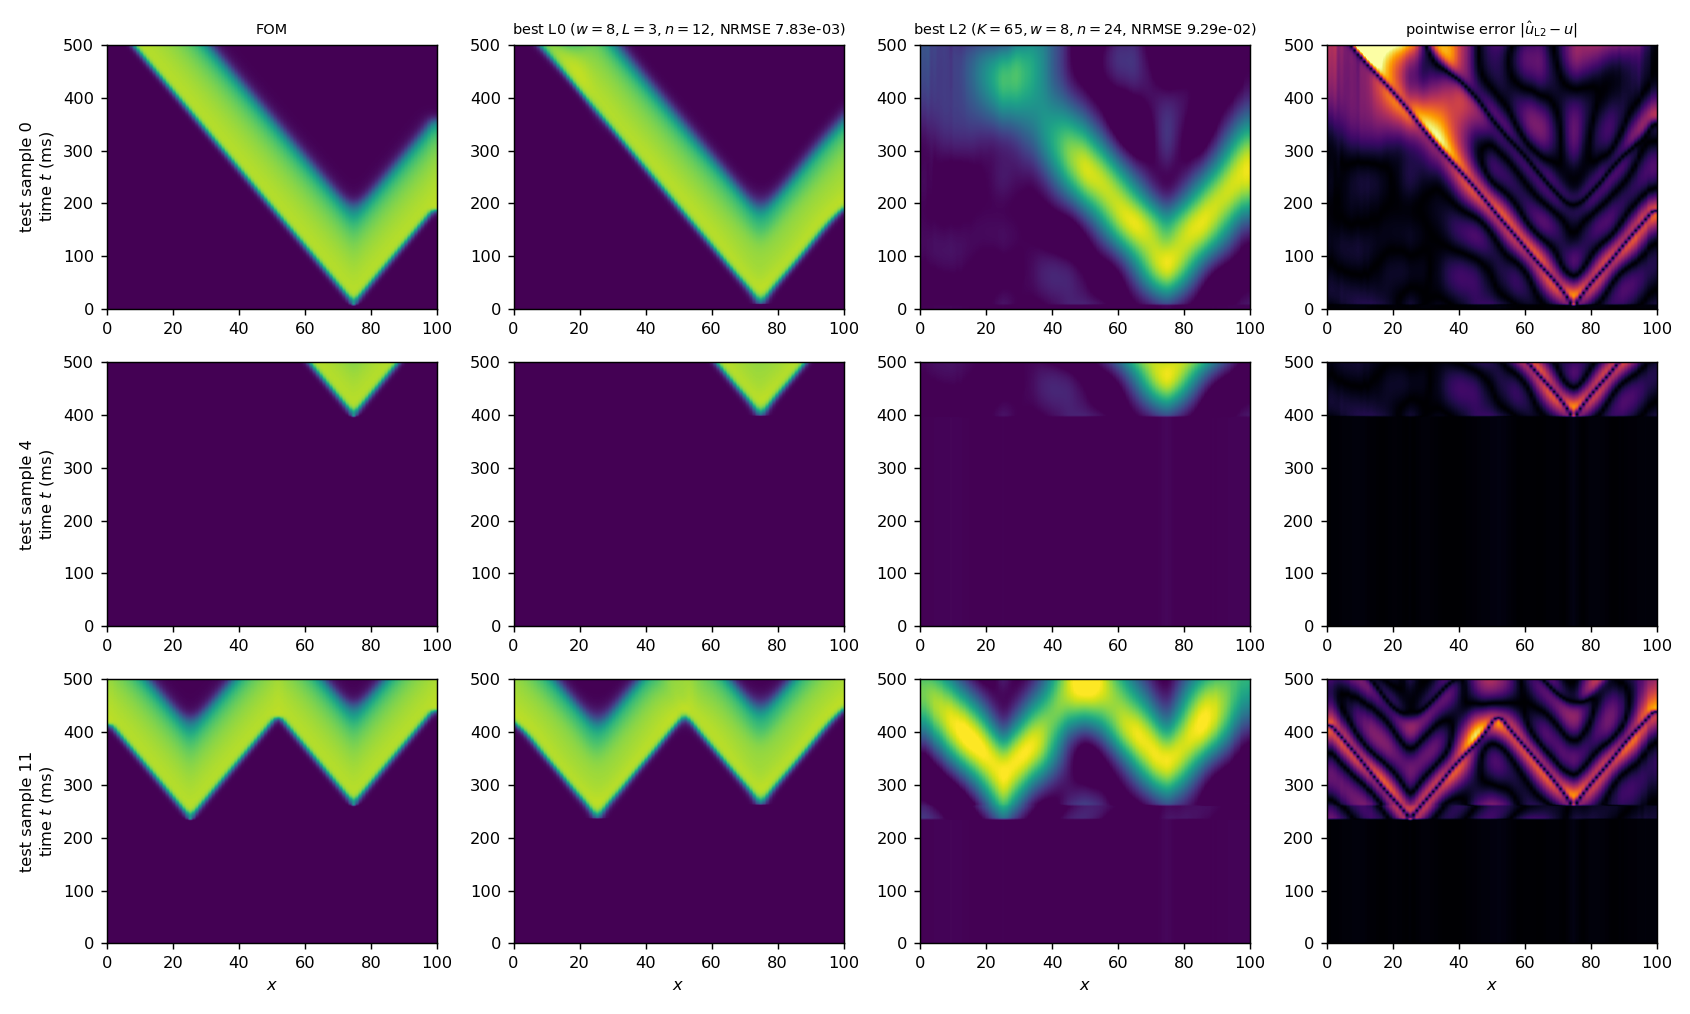
\includegraphics[width=0.90\textwidth,height=0.215\textheight,keepaspectratio]{fig9_C_fronts_comparison.png}
  \caption{Case C space-time transmembrane potential $u(x,t)$ on three test trajectories (rows: test samples 0, 4, and 11) at the $10{,}000$-iteration BFGS budget. \textbf{Columns:} FOM ground truth; best $\mathrm{L0}$ configuration ($w=8, L=3, n=12$, seed 0 $\NRMSE = 7.10\cdot 10^{-3}$); best $\mathrm{L2}$ configuration on test ($K=65, w=8, L=1, n=24$, seed 0 $\NRMSE = 9.29\cdot 10^{-2}$); and pointwise absolute error $|\hat{u}_{\mathrm{L2}}(x,t) - u(x,t)|$, demonstrating how linear polynomial synthesis concentrates error along the moving depolarisation wave fronts and generates global Gibbs oscillations.}
  \label{fig:rq2bis_fig9}
\end{figure}

\subsection{The Iteration Surface \texorpdfstring{$\NRMSE(w, \text{iterations})$}{NRMSE(w, iterations)} and 1,000 vs.\ 10,000 Iterations}

Figures~\ref{fig:rq2bis_fig2}, \ref{fig:rq2bis_fig4}, and~\ref{fig:rq2bis_fig6} and Table~\ref{tab:rq2bis_checkpoints} present the evolution of the test NRMSE across the nine BFGS checkpoints~\eqref{eq:checkpoints}, alongside the direct comparison between the $1{,}000$-iteration laptop pilot and the $10{,}000$-iteration CINECA Leonardo cluster sweep.

\begin{figure}[!htbp]
  \centering
  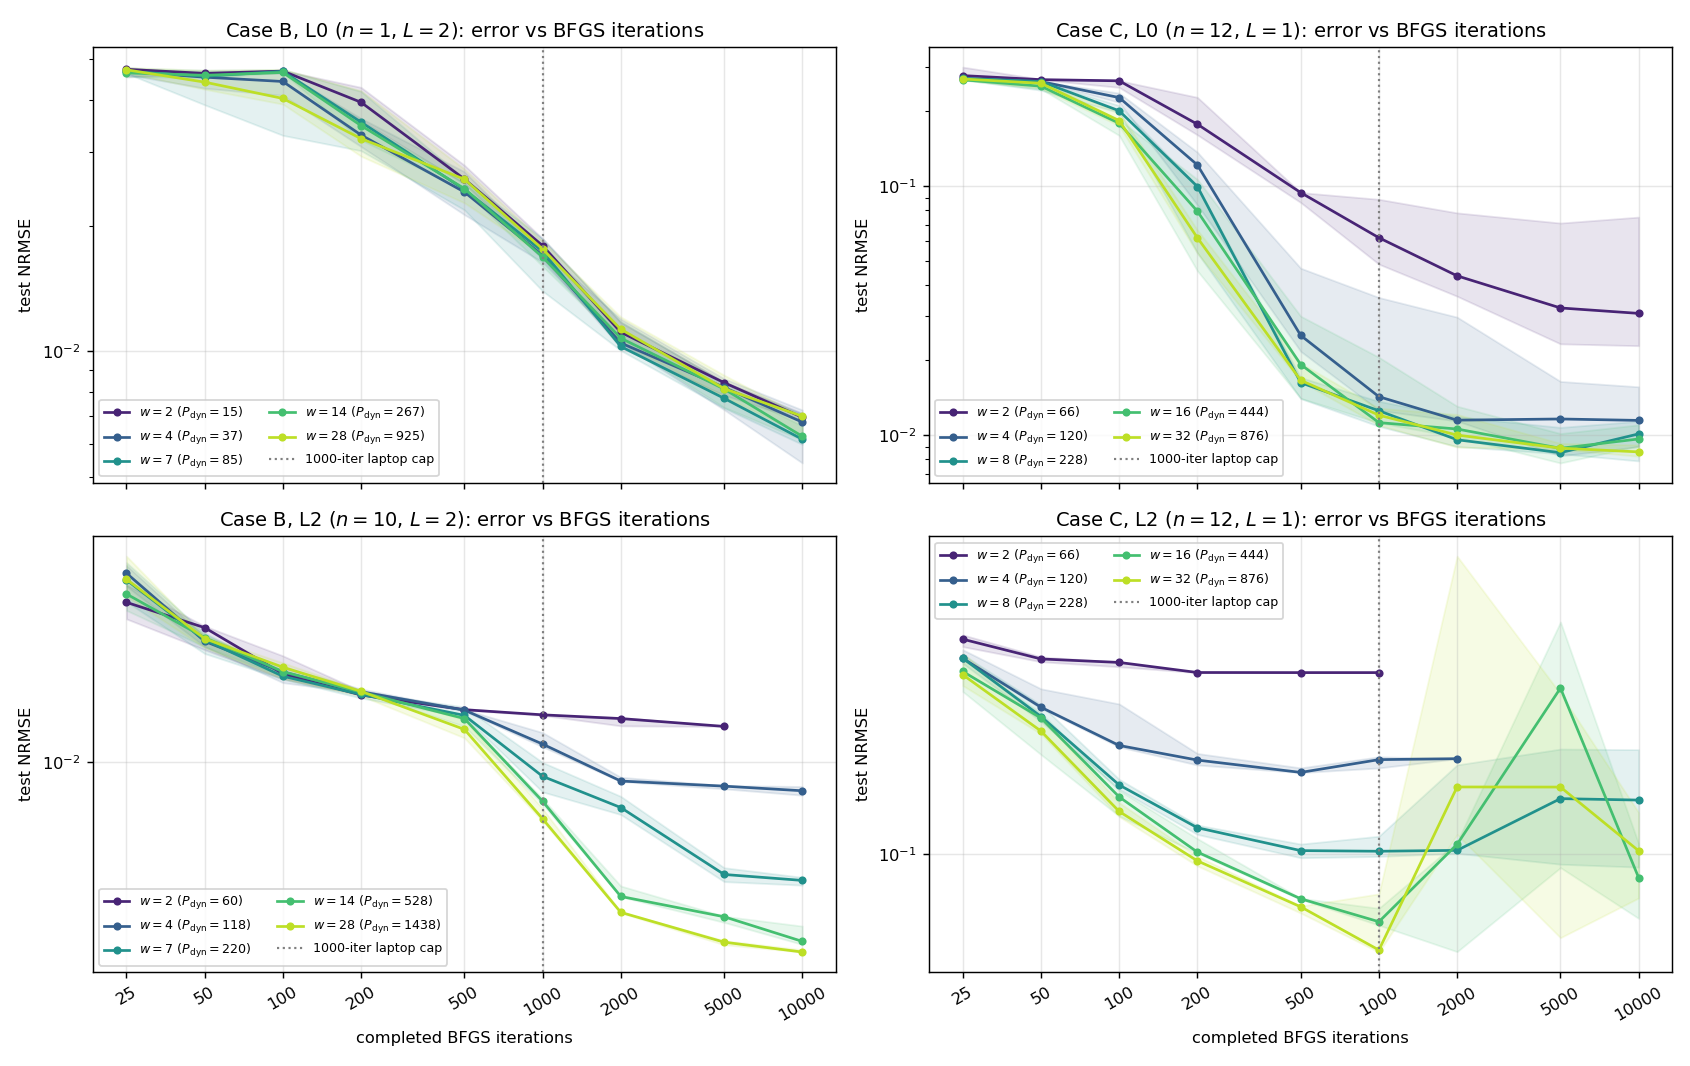
\includegraphics[width=0.90\textwidth,height=0.215\textheight,keepaspectratio]{fig2_iteration_surface.png}
  \caption{Stage~3 quasi-Newton iteration surface: test NRMSE (median and min--max band of 3 seeds) as a function of completed BFGS iterations $k \in \{25, 50, 100, 200, 500, 1000, 2000, 5000, 10000\}$ across dynamics hidden widths $w$, for Case~B (\textbf{left}) and Case~C (\textbf{right}), in the nonlinear arm $\mathrm{L0}$ (\textbf{top}) and linear arm $\mathrm{L2}$ (\textbf{bottom}). The vertical dotted line indicates the $1{,}000$-iteration pilot cap.}
  \label{fig:rq2bis_fig2}
\end{figure}

\begin{figure}[!htbp]
  \centering
  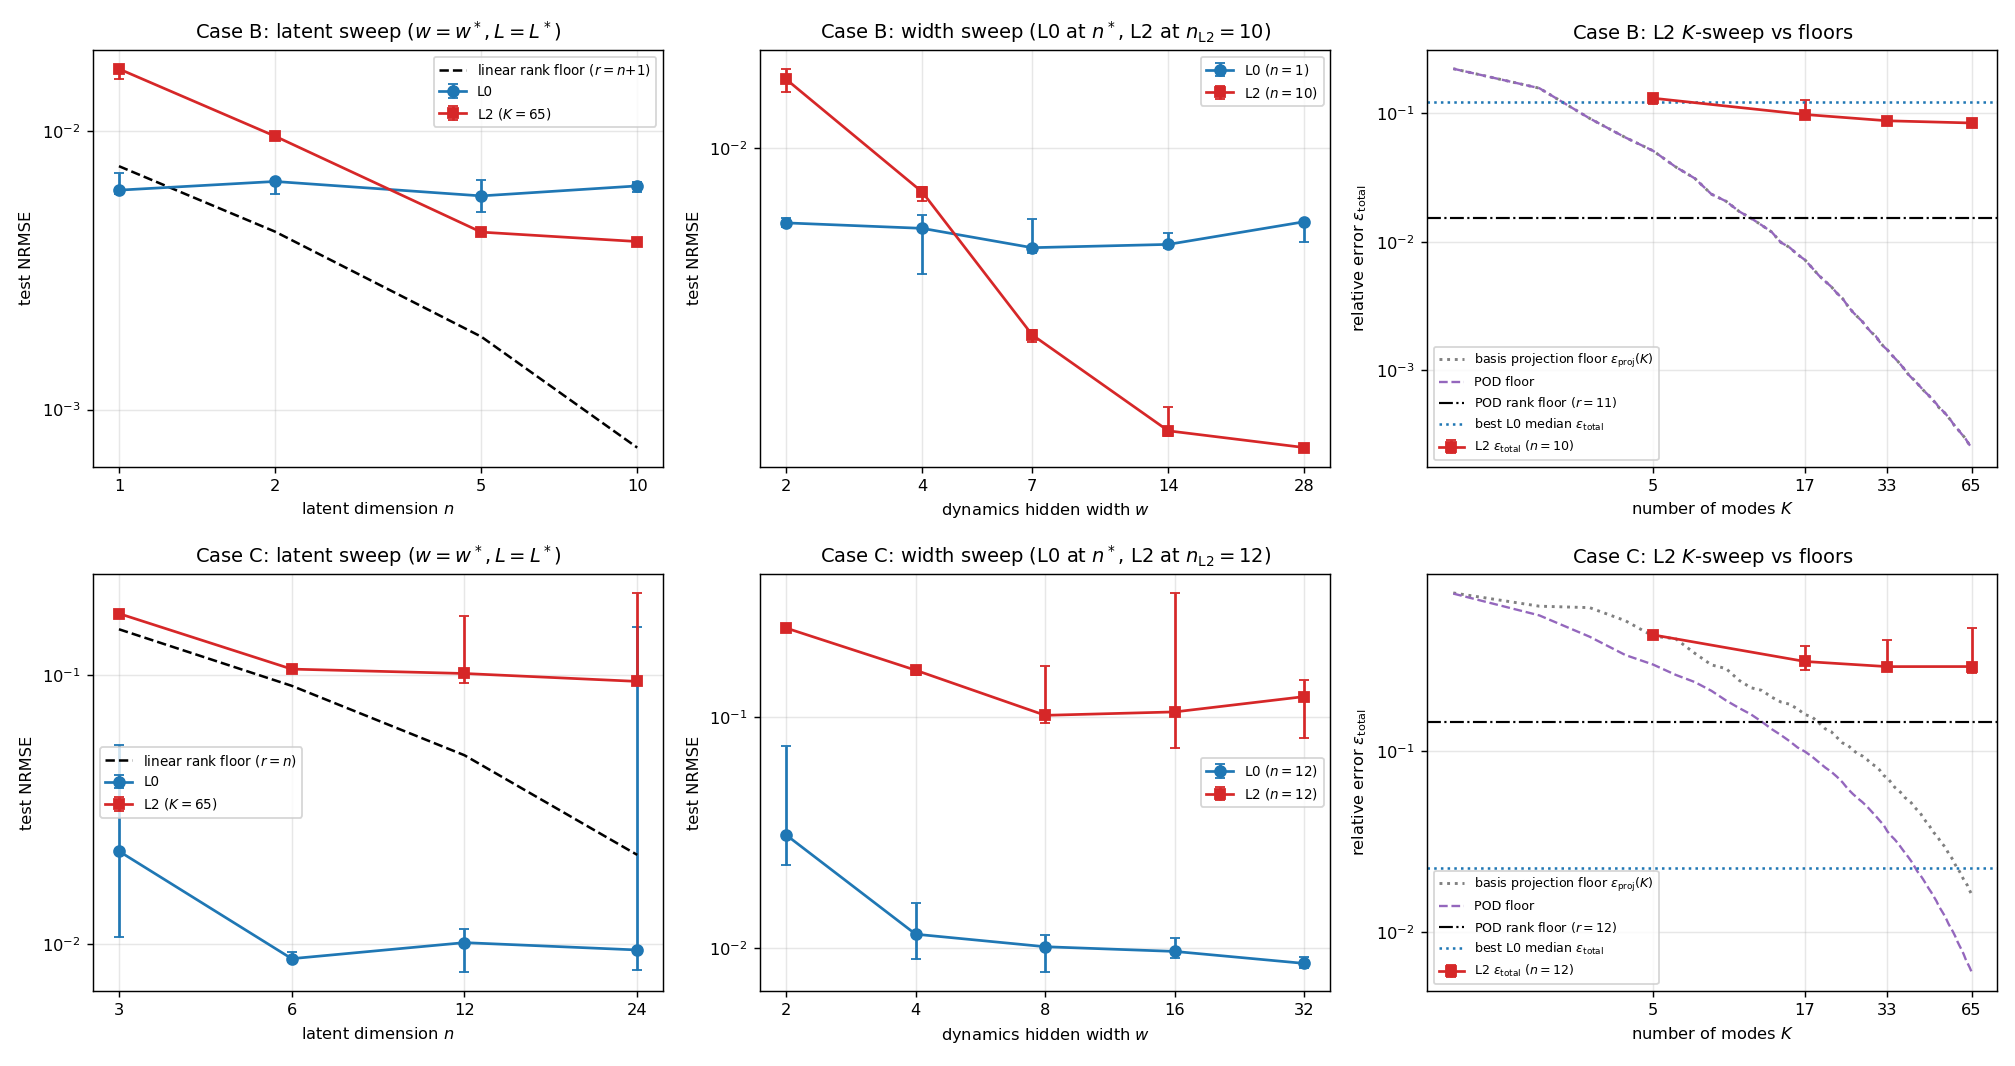
\includegraphics[width=0.90\textwidth,height=0.215\textheight,keepaspectratio]{fig4_linear_arm_sweeps.png}
  \caption{Stage~7 linear reconstructor arm ($\mathrm{L2}$, red squares) versus nonlinear reconstructor arm ($\mathrm{L0}$, blue circles) at $10{,}000$ BFGS iterations in Case~B (\textbf{top row}) and Case~C (\textbf{bottom row}): test NRMSE against latent dimension $n$ with the POD rank floor (left), against dynamics hidden width $w$ (centre), and relative test error $\varepsilon_{\mathrm{total}}$ against basis size $K$ compared with $\varepsilon_{\mathrm{proj}}(K)$ and the POD rank floor (right).}
  \label{fig:rq2bis_fig4}
\end{figure}

\begin{figure}[!htbp]
  \centering
  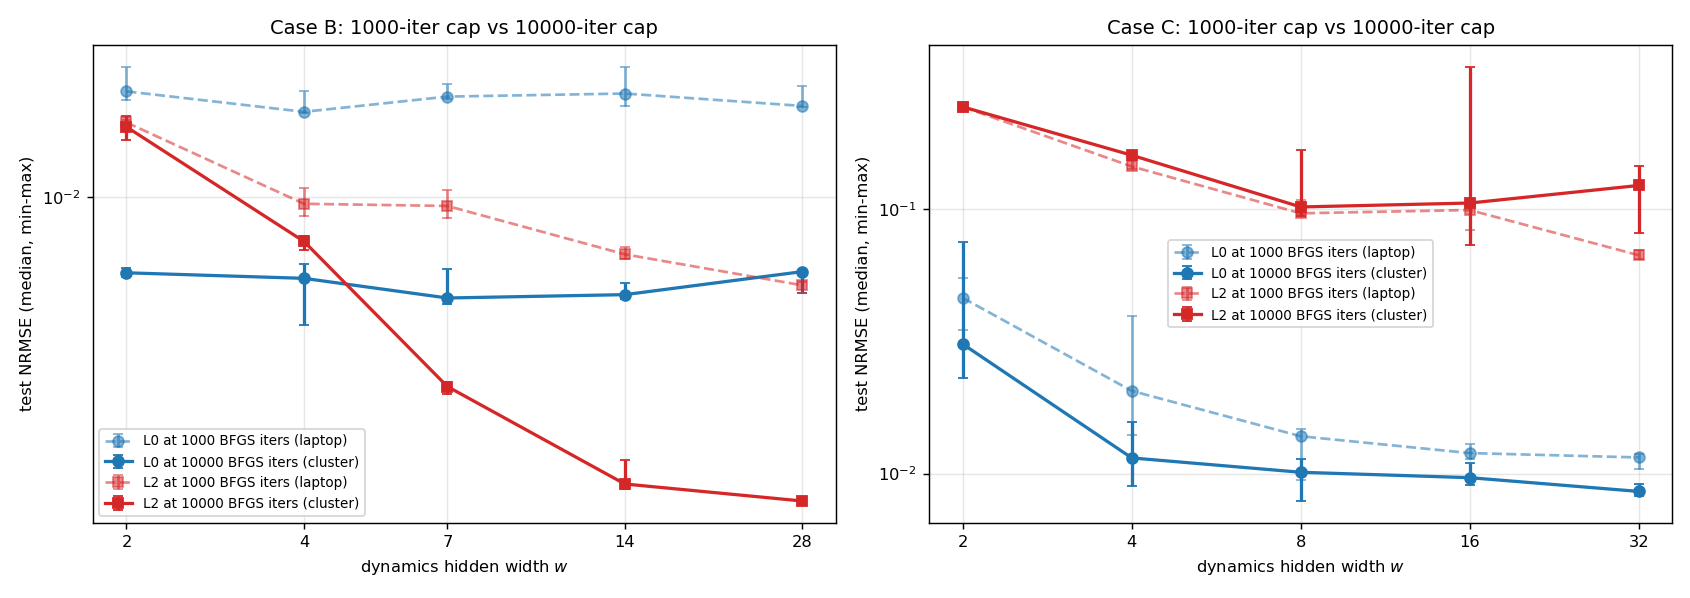
\includegraphics[width=0.90\textwidth,height=0.215\textheight,keepaspectratio]{fig6_budget_1000_vs_10000.png}
  \caption{Impact of the tenfold increase in quasi-Newton budget from the $1{,}000$-iteration laptop sweep (dashed curves) to the $10{,}000$-iteration CINECA Leonardo cluster sweep (solid curves) across the dynamics width sweeps of Case~B (\textbf{left}) and Case~C (\textbf{right}).}
  \label{fig:rq2bis_fig6}
\end{figure}

\begin{table}[!htbp]
\centering
\caption{Stage~3 checkpoint evolution: median test NRMSE across completed BFGS iterations $k \in \{50, 200, 500, 1000, 2000, 5000, 10000\}$ on the dynamics width sweeps of Cases~B and~C, together with the relative error reduction between iteration $1{,}000$ and iteration $10{,}000$.}
\label{tab:rq2bis_checkpoints}
\footnotesize\resizebox{\textwidth}{!}{%

\begin{tabular}{@{}llrrrrrrrrr@{}}
\toprule
\textbf{Case \& Arm} & $w$ & $P_{\mathrm{dyn}}$ & \textbf{iter 50} & \textbf{iter 200} & \textbf{iter 500} & \textbf{iter 1000} & \textbf{iter 2000} & \textbf{iter 5000} & \textbf{iter 10000} & \textbf{Drop $1\text{k}\to 10\text{k}$} \\
\midrule
\textbf{B, L0} ($n{=}1, L{=}2$)
 & $2$  & $15$  & $4.63\cdot 10^{-2}$ & $3.95\cdot 10^{-2}$ & $2.58\cdot 10^{-2}$ & $1.79\cdot 10^{-2}$ & $1.11\cdot 10^{-2}$ & $8.40\cdot 10^{-3}$ & $6.94\cdot 10^{-3}$ & $\mathbf{+61.2\%}$ \\
 & $4$  & $37$  & $4.54\cdot 10^{-2}$ & $3.30\cdot 10^{-2}$ & $2.41\cdot 10^{-2}$ & $1.70\cdot 10^{-2}$ & $1.05\cdot 10^{-2}$ & $8.19\cdot 10^{-3}$ & $6.76\cdot 10^{-3}$ & $\mathbf{+60.2\%}$ \\
 & $7$  & $85$  & $4.56\cdot 10^{-2}$ & $3.54\cdot 10^{-2}$ & $2.44\cdot 10^{-2}$ & $1.73\cdot 10^{-2}$ & $1.03\cdot 10^{-2}$ & $7.71\cdot 10^{-3}$ & $6.15\cdot 10^{-3}$ & $\mathbf{+64.5\%}$ \\
 & $14$ & $267$ & $4.58\cdot 10^{-2}$ & $3.47\cdot 10^{-2}$ & $2.45\cdot 10^{-2}$ & $1.68\cdot 10^{-2}$ & $1.07\cdot 10^{-2}$ & $8.11\cdot 10^{-3}$ & $6.25\cdot 10^{-3}$ & $\mathbf{+62.8\%}$ \\
 & $28$ & $925$ & $4.41\cdot 10^{-2}$ & $3.23\cdot 10^{-2}$ & $2.58\cdot 10^{-2}$ & $1.76\cdot 10^{-2}$ & $1.13\cdot 10^{-2}$ & $8.13\cdot 10^{-3}$ & $6.98\cdot 10^{-3}$ & $\mathbf{+60.3\%}$ \\
\midrule
\textbf{B, L2} ($n{=}10, K{=}65$)
 & $2$  & $60$   & $2.80\cdot 10^{-2}$ & $1.67\cdot 10^{-2}$ & $1.49\cdot 10^{-2}$ & $1.43\cdot 10^{-2}$ & $1.39\cdot 10^{-2}$ & $1.31\cdot 10^{-2}$ & $1.40\cdot 10^{-2}$ (st) & $+2.1\%$ \\
 & $4$  & $118$  & $2.52\cdot 10^{-2}$ & $1.71\cdot 10^{-2}$ & $1.49\cdot 10^{-2}$ & $1.15\cdot 10^{-2}$ & $8.62\cdot 10^{-3}$ & $8.29\cdot 10^{-3}$ & $8.07\cdot 10^{-3}$ & $\mathbf{+30.1\%}$ \\
 & $7$  & $220$  & $2.55\cdot 10^{-2}$ & $1.68\cdot 10^{-2}$ & $1.43\cdot 10^{-2}$ & $8.94\cdot 10^{-3}$ & $7.03\cdot 10^{-3}$ & $4.21\cdot 10^{-3}$ & $4.02\cdot 10^{-3}$ & $\mathbf{+55.0\%}$ \\
 & $14$ & $528$  & $2.59\cdot 10^{-2}$ & $1.71\cdot 10^{-2}$ & $1.39\cdot 10^{-2}$ & $7.38\cdot 10^{-3}$ & $3.55\cdot 10^{-3}$ & $3.04\cdot 10^{-3}$ & $2.52\cdot 10^{-3}$ & $\mathbf{+65.9\%}$ \\
 & $28$ & $1438$ & $2.57\cdot 10^{-2}$ & $1.72\cdot 10^{-2}$ & $1.28\cdot 10^{-2}$ & $6.45\cdot 10^{-3}$ & $3.15\cdot 10^{-3}$ & $2.50\cdot 10^{-3}$ & $2.32\cdot 10^{-3}$ & $\mathbf{+64.1\%}$ \\
\midrule
\textbf{C, L0} ($n{=}12, L{=}1$)
 & $2$  & $66$  & $2.68\cdot 10^{-1}$ & $1.77\cdot 10^{-1}$ & $9.42\cdot 10^{-2}$ & $6.21\cdot 10^{-2}$ & $4.36\cdot 10^{-2}$ & $3.24\cdot 10^{-2}$ & $3.08\cdot 10^{-2}$ & $\mathbf{+50.3\%}$ \\
 & $4$  & $120$ & $2.63\cdot 10^{-1}$ & $1.22\cdot 10^{-1}$ & $2.52\cdot 10^{-2}$ & $1.43\cdot 10^{-2}$ & $1.15\cdot 10^{-2}$ & $1.16\cdot 10^{-2}$ & $1.15\cdot 10^{-2}$ & $\mathbf{+19.7\%}$ \\
 & $8$  & $228$ & $2.63\cdot 10^{-1}$ & $9.97\cdot 10^{-2}$ & $1.63\cdot 10^{-2}$ & $1.25\cdot 10^{-2}$ & $9.58\cdot 10^{-3}$ & $8.50\cdot 10^{-3}$ & $1.01\cdot 10^{-2}$ & $\mathbf{+19.3\%}$ \\
 & $16$ & $444$ & $2.52\cdot 10^{-1}$ & $7.93\cdot 10^{-2}$ & $1.92\cdot 10^{-2}$ & $1.12\cdot 10^{-2}$ & $1.06\cdot 10^{-2}$ & $8.85\cdot 10^{-3}$ & $9.65\cdot 10^{-3}$ & $\mathbf{+14.0\%}$ \\
 & $32$ & $876$ & $2.59\cdot 10^{-1}$ & $6.21\cdot 10^{-2}$ & $1.66\cdot 10^{-2}$ & $1.20\cdot 10^{-2}$ & $1.00\cdot 10^{-2}$ & $8.86\cdot 10^{-3}$ & $8.57\cdot 10^{-3}$ & $\mathbf{+28.8\%}$ \\
\midrule
\textbf{C, L2} ($n{=}12, K{=}65$)
 & $2$  & $66$  & $2.59\cdot 10^{-1}$ & $2.43\cdot 10^{-1}$ & $2.43\cdot 10^{-1}$ & $2.43\cdot 10^{-1}$ & -- & -- & $2.43\cdot 10^{-1}$ (st) & $0.0\%$ \\
 & $4$  & $120$ & $2.05\cdot 10^{-1}$ & $1.58\cdot 10^{-1}$ & $1.49\cdot 10^{-1}$ & $1.59\cdot 10^{-1}$ & $1.59\cdot 10^{-1}$ & -- & $1.59\cdot 10^{-1}$ (st) & $-0.4\%$ \\
 & $8$  & $228$ & $1.96\cdot 10^{-1}$ & $1.14\cdot 10^{-1}$ & $1.02\cdot 10^{-1}$ & $1.01\cdot 10^{-1}$ & $1.02\cdot 10^{-1}$ & $1.31\cdot 10^{-1}$ & $1.02\cdot 10^{-1}$ & $-0.3\%$ \\
 & $16$ & $444$ & $1.94\cdot 10^{-1}$ & $1.01\cdot 10^{-1}$ & $8.04\cdot 10^{-2}$ & $\mathbf{7.18\cdot 10^{-2}}$ & $1.05\cdot 10^{-1}$ & $2.25\cdot 10^{-1}$ & $1.05\cdot 10^{-1}$ & $\mathbf{-46.3\%}$ (overfit) \\
 & $32$ & $876$ & $1.82\cdot 10^{-1}$ & $9.67\cdot 10^{-2}$ & $7.73\cdot 10^{-2}$ & $\mathbf{6.26\cdot 10^{-2}}$ & $1.39\cdot 10^{-1}$ & $1.39\cdot 10^{-1}$ & $1.22\cdot 10^{-1}$ & $\mathbf{-95.8\%}$ (overfit) \\
\bottomrule
\end{tabular}
}
\end{table}

Table~\ref{tab:rq2bis_checkpoints} and Figure~\ref{fig:rq2bis_fig2} demonstrate why stopping quasi-Newton optimization at $500$ or $1{,}000$ iterations distorts architectural comparisons:
\begin{itemize}[leftmargin=2em]
  \item Between iteration $1{,}000$ and iteration $10{,}000$, every Case~B $\mathrm{L0}$ configuration drops by a further \textbf{$60.2\%$ to $64.5\%$} (from $\sim 1.7\cdot 10^{-2}$ down to $6.15$--$6.98\cdot 10^{-3}$), and every wide Case~B $\mathrm{L2}$ configuration ($w \in \{7, 14, 28\}$) drops by a further \textbf{$55.0\%$ to $65.9\%$} (from $8.94, 7.38, 6.45\cdot 10^{-3}$ down to $4.02, 2.52, 2.32\cdot 10^{-3}$). At iteration $500$, the five widths of Case~B $\mathrm{L2}$ were still bunched tightly between $1.28\cdot 10^{-2}$ and $1.49\cdot 10^{-2}$; only between iterations $1{,}000$ and $10{,}000$ does the $6\times$ capacity separation between $w=2$ ($1.40\cdot 10^{-2}$) and $w=28$ ($2.32\cdot 10^{-3}$) fully emerge!
  \item In Case~C $\mathrm{L0}$, at iteration $500$ the width curve is non-monotone ($[0.0942, 0.0252, 0.0163, 0.0192, 0.0166]$), because the larger networks ($w=16, 32$) have more parameters ($P_{\mathrm{total}} = 1924, 2356$) and require more quasi-Newton rank-2 updates to build an accurate inverse-Hessian approximation (Hypothesis~H3). By iteration $10{,}000$, all five widths have converged and the curve becomes strictly monotone decreasing ($[0.0308, 0.0115, 0.0101, 0.00965, 0.00857]$), falsifying Hypothesis~H3 at $10{,}000$ iterations in Case~C $\mathrm{L0}$ while still supporting it in Case~B $\mathrm{L0}$ (where the largest network $w=28, P_{\mathrm{total}} = 2895$ remains slightly above $w=7$, $6.98\cdot 10^{-3}$ vs.\ $6.15\cdot 10^{-3}$).
\end{itemize}

\subsection{Empirical Verification of the Dynamics Bottleneck Rank Bound (\texorpdfstring{$\mathrm{H4}$}{H4})}

To test Proposition~\ref{prop:dyn_rank_bound} directly on the trained models of \texttt{RQ2-bis}, we rebuilt all stored $\mathrm{L0}$ and $\mathrm{L2}$ networks in pure NumPy from \texttt{results/weights/}, rolled out the test-set latent trajectories $S_{\mathrm{traj}} \in \R^{(S_{\mathrm{test}} N_t) \times n}$, computed the exact analytical state-transition Jacobians $J(\mathbf{s}^{(s)}(t_i), \mathbf{u}^{(s)}(t_i)) = \partial\dot{\mathbf{s}}/\partial\mathbf{s} \in \R^{n \times n}$, and evaluated the numerical rank (number of singular values $\sigma_k > 10^{-3}\sigma_1$) of both matrices across all three seeds. Figure~\ref{fig:rq2bis_fig7} and Table~\ref{tab:rq2bis_ranks} report the results.

\begin{figure}[!htbp]
  \centering
  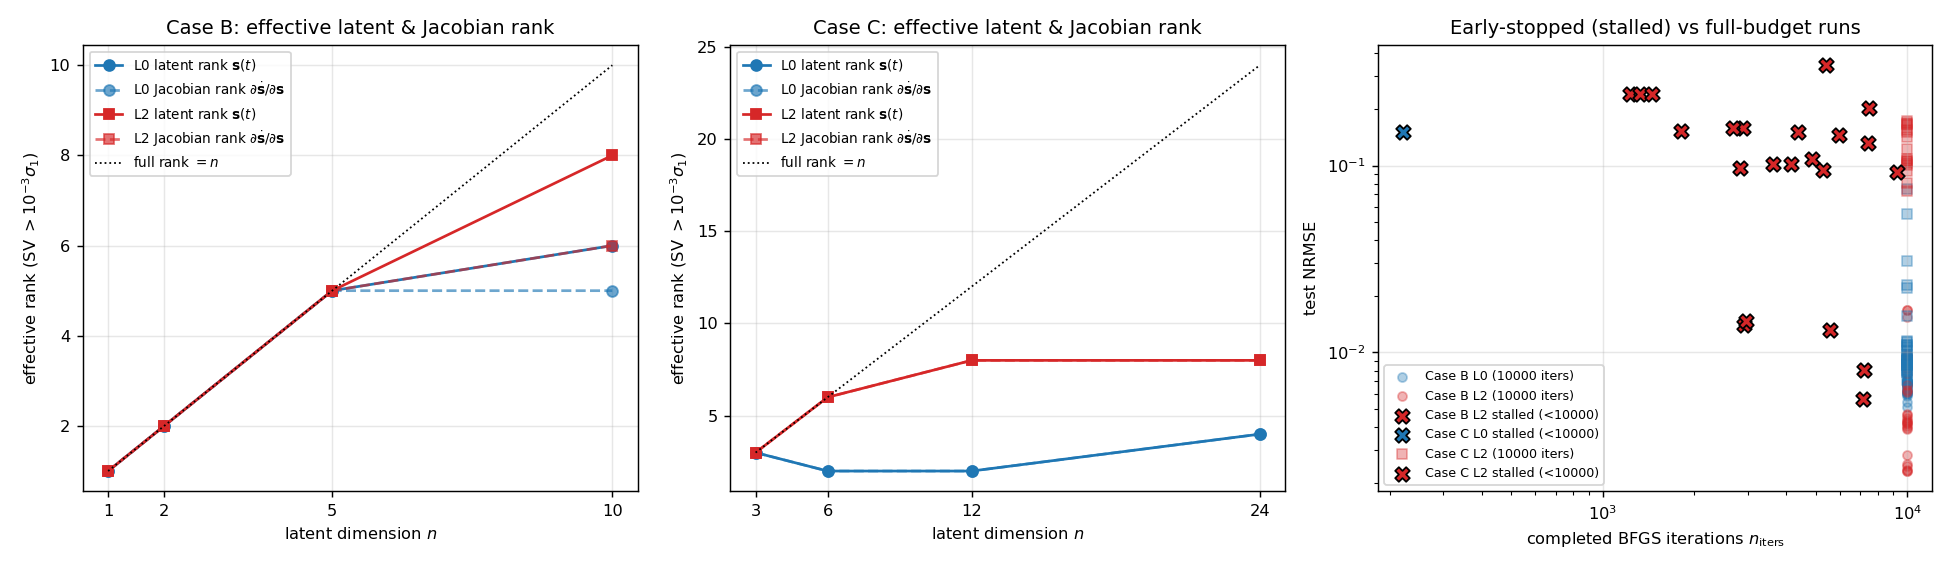
\includegraphics[width=0.90\textwidth,height=0.215\textheight,keepaspectratio]{fig7_ranks_and_stalls.png}
  \caption{\textbf{Left and centre:} empirical SVD rank (number of singular values $> 10^{-3}\sigma_1$, median over 3 seeds) of the test latent trajectories $\mathbf{s}(t)$ (solid lines) and of the state-transition Jacobians $\partial\dot{\mathbf{s}}/\partial\mathbf{s}$ (dashed lines) as a function of latent dimension $n$ at canonical dynamics hidden width ($w^*=7$ in Case~B, $w^*=8$ in Case~C). Both hit the exact algebraic ceiling of Proposition~\ref{prop:dyn_rank_bound}. \textbf{Right:} final test NRMSE versus completed BFGS iterations $n_{\mathrm{iters}}$ across all 126 cluster runs, highlighting the 23 early-stopped (\texttt{stalled}) runs.}
  \label{fig:rq2bis_fig7}
\end{figure}

\begin{table}[!htbp]
\centering
\caption{Empirical SVD rank (singular values $> 10^{-3}\sigma_1$ across seeds $[s_0, s_1, s_2]$) and smallest-to-largest singular-value ratio $\sigma_n/\sigma_1$ of the test latent trajectories $S_{\mathrm{traj}}$ and dynamics Jacobians $\partial\dot{\mathbf{s}}/\partial\mathbf{s}$, compared against the theoretical structural ceiling of Proposition~\ref{prop:dyn_rank_bound}.}
\label{tab:rq2bis_ranks}
\footnotesize\resizebox{\textwidth}{!}{%

\begin{tabular}{@{}llrrcllrr@{}}
\toprule
\textbf{Case} & \textbf{Arm} & \textbf{Width $w$} & \textbf{Latent $n$} & \textbf{Prop.~\ref{prop:dyn_rank_bound} Ceiling} & \textbf{Traj.\ Rank $[s_0,s_1,s_2]$} & \textbf{Jac.\ Rank $[s_0,s_1,s_2]$} & \textbf{Med.\ $\frac{\sigma_n}{\sigma_1}(\mathbf{s})$} & \textbf{Med.\ $\frac{\sigma_n}{\sigma_1}(J)$} \\
\midrule
\textbf{B} & L0 & $7$ ($w^*$) & $1$ & $1$ & $[1, 1, 1]$ & $[1, 1, 1]$ & $1.00$ & $1.00$ \\
 & L0 & $7$ ($w^*$) & $2$ & $2$ & $[2, 2, 2]$ & $[2, 2, 2]$ & $1.33\cdot 10^{-1}$ & $2.25\cdot 10^{-1}$ \\
 & L0 & $7$ ($w^*$) & $5$ & $5$ & $[5, 5, 5]$ & $[4, 5, 5]$ & $4.49\cdot 10^{-3}$ & $1.63\cdot 10^{-2}$ \\
 & L0 & $7$ ($w^*$) & $10$ & $\mathbf{8}$ ($w^*+1$) & $\mathbf{[6, 7, 6]}$ & $\mathbf{[5, 5, 6]}$ & $\mathbf{9.23\cdot 10^{-17}}$ & $\mathbf{5.25\cdot 10^{-18}}$ \\
 & L2 & $7$ ($w^*$) & $1$ & $1$ & $[1, 1, 1]$ & $[1, 1, 1]$ & $1.00$ & $1.00$ \\
 & L2 & $7$ ($w^*$) & $2$ & $2$ & $[2, 2, 2]$ & $[2, 2, 2]$ & $4.84\cdot 10^{-1}$ & $1.83\cdot 10^{-1}$ \\
 & L2 & $7$ ($w^*$) & $5$ & $5$ & $[5, 5, 5]$ & $[5, 5, 5]$ & $2.19\cdot 10^{-2}$ & $3.67\cdot 10^{-2}$ \\
 & L2 & $7$ ($w^*$) & $10$ & $\mathbf{8}$ ($w^*+1$) & $\mathbf{[8, 7, 8]}$ & $\mathbf{[5, 6, 6]}$ & $\mathbf{1.21\cdot 10^{-16}}$ & $\mathbf{5.83\cdot 10^{-18}}$ \\
 & \textbf{L2} & $\mathbf{28}$ ($4w^*$) & $\mathbf{10}$ & $\mathbf{10}$ & $\mathbf{[10, 10, 10]}$ & $\mathbf{[10, 10, 10]}$ & $> 10^{-3}$ & $> 10^{-3}$ \\
\midrule
\textbf{C} & L0 & $8$ ($w^*$) & $3$ & $3$ & $[3, 2, 3]$ & $[3, 2, 3]$ & $3.07\cdot 10^{-2}$ & $1.29\cdot 10^{-1}$ \\
 & L0 & $8$ ($w^*$) & $6$ & $6$ & $\mathbf{[2, 2, 2]}$ & $\mathbf{[2, 2, 2]}$ & $6.16\cdot 10^{-7}$ & $1.00\cdot 10^{-6}$ \\
 & L0 & $8$ ($w^*$) & $12$ & $\mathbf{8}$ ($w^*$) & $\mathbf{[2, 3, 2]}$ & $\mathbf{[2, 4, 2]}$ & $\mathbf{6.46\cdot 10^{-17}}$ & $\mathbf{2.18\cdot 10^{-18}}$ \\
 & L0 & $8$ ($w^*$) & $24$ & $\mathbf{8}$ ($w^*$) & $\mathbf{[4, 5, 3]}$ & $\mathbf{[4, 8, 3]}$ & $\mathbf{1.98\cdot 10^{-17}}$ & $\mathbf{4.67\cdot 10^{-19}}$ \\
 & \textbf{L0} & $\mathbf{32}$ ($4w^*$) & $\mathbf{12}$ & $\mathbf{12}$ & $\mathbf{[4, 3, 5]}$ & $\mathbf{[4, 4, 4]}$ & $< 10^{-3}$ & $< 10^{-3}$ \\
 & L2 & $8$ ($w^*$) & $3$ & $3$ & $[3, 3, 3]$ & $[3, 3, 3]$ & $2.31\cdot 10^{-1}$ & $1.63\cdot 10^{-1}$ \\
 & L2 & $8$ ($w^*$) & $6$ & $6$ & $[6, 6, 6]$ & $[6, 6, 6]$ & $1.09\cdot 10^{-1}$ & $8.86\cdot 10^{-2}$ \\
 & L2 & $8$ ($w^*$) & $12$ & $\mathbf{8}$ ($w^*$) & $\mathbf{[8, 8, 8]}$ & $\mathbf{[8, 8, 8]}$ & $\mathbf{7.82\cdot 10^{-16}}$ & $\mathbf{9.41\cdot 10^{-18}}$ \\
 & L2 & $8$ ($w^*$) & $24$ & $\mathbf{8}$ ($w^*$) & $\mathbf{[8, 8, 8]}$ & $\mathbf{[8, 8, 8]}$ & $\mathbf{5.16\cdot 10^{-17}}$ & $\mathbf{1.66\cdot 10^{-18}}$ \\
 & \textbf{L2} & $\mathbf{32}$ ($4w^*$) & $\mathbf{12}$ & $\mathbf{12}$ & $\mathbf{[12, 12, 12]}$ & $\mathbf{[12, 12, 12]}$ & $> 10^{-3}$ & $> 10^{-3}$ \\
\bottomrule
\end{tabular}
}
\end{table}

Table~\ref{tab:rq2bis_ranks} provides a textbook confirmation of both physical manifold collapse and Proposition~\ref{prop:dyn_rank_bound}:
\begin{enumerate}[leftmargin=2em]
  \item \textbf{Exact saturation of the algebraic dynamics bottleneck in $\mathrm{L2}$:} Because the linear decoder $\mathrm{L2}$ can only reduce error by spanning as many independent linear directions as possible (Proposition~\ref{prop:rec_rank_bound}), it uses every single latent dimension available at $n=3$ ($[3,3,3]$) and $n=6$ ($[6,6,6]$) in Case~C, and at $n=1,2,5$ in Case~B. When $n$ is raised to $12$ and $24$ at the canonical width $w^* = 8$ in Case~C, \textbf{both the trajectory rank and the Jacobian rank hit the exact theoretical wall $\min(n, w^*) = 8$ across all three seeds ($[8,8,8]$)}, with the remaining $n - 8$ singular values dropping to machine precision ($\sigma_n/\sigma_1 \approx 10^{-16}$ to $10^{-18}$)! Similarly, in Case~B $\mathrm{L2}$ at $w^* = 7, n = 10$, the trajectory rank hits the exact ceiling $w^* + 1 = 8$ ($[8,7,8]$, $\sigma_{10}/\sigma_1 = 1.21\cdot 10^{-16}$) and the Jacobian rank is bounded by $w^* = 7$ ($[5,6,6]$). The instant $\NNdyn$ is widened to $w = 28$ in Case~B or $w = 32$ in Case~C, the structural bottleneck disappears and $\mathrm{L2}$ immediately expands to full rank \textbf{$[10,10,10]$} in Case~B and \textbf{$[12,12,12]$} in Case~C! This explains why increasing $n$ from $5$ to $10$ at $w^*=7$ in Case~B $\mathrm{L2}$ lowered test NRMSE by only $7\%$ ($4.34\cdot 10^{-3} \to 4.02\cdot 10^{-3}$), whereas widening $w$ to $28$ at $n=10$ reduced the error by another $42\%$ to $2.32\cdot 10^{-3}$.
  \item \textbf{Intrinsic low-rank manifold collapse in Case C $\mathrm{L0}$:} In stark contrast to $\mathrm{L2}$, Case~C $\mathrm{L0}$ collapses its latent trajectories to an effective rank of \textbf{only $2$ to $5$} even when no algebraic bottleneck is active: at $w^*=8, n=6$ (where the algebraic ceiling is $6$), $\mathrm{L0}$ uses rank $[2,2,2]$ ($\sigma_6/\sigma_1 = 6.16\cdot 10^{-7}$), and even when widened to $w=32, n=12$ (where the algebraic ceiling is $12$), $\mathrm{L0}$ uses only rank \textbf{$[4,3,5]$}! Because $\NNrec(\mathbf{s},x)$ is a nonlinear coordinate chart that translates the sharp wave profiles directly, it requires only $2$ to $5$ active latent coordinates to track the wave positions and recovery state, automatically pruning the redundant $n - 5$ latent directions during BFGS optimization.
\end{enumerate}

\section{Scalability in Terms of FLOPs, Hardware Throughput, and Error}
\label{sec:flops}

A central objective of this paper is to establish the precise computational trade-off between approximation error and arithmetic cost---measured both in floating-point operations (FLOPs) and in multi-core wall-clock execution time on the CINECA Leonardo supercomputer---when the nonlinear pointwise reconstructor $\mathrm{L0}$ is replaced by the linear modal reconstructor $\mathrm{L2}$ or when the dynamics network $\NNdyn$ is scaled in width, depth, and iteration budget. Comparing $\mathrm{L0}$ and $\mathrm{L2}$ solely on the number of BFGS iterations $n_{\mathrm{iters}}$ or function/gradient evaluations $n_{\mathrm{fev}}$ is fundamentally misleading, because one evaluation of $\mathrm{L0}$ and one evaluation of $\mathrm{L2}$ perform vastly different amounts of arithmetic and exhibit completely different hardware execution profiles.

\subsection{Analytical Derivation of Forward and Backward FLOPs per Evaluation}
\label{sec:flops_derivation}

Let a training split comprise $S$ trajectories, $N_t$ time steps ($N_t - 1$ Forward Euler steps), $N_x$ spatial query points per snapshot $(s,t_i)$, and $n_{\mathrm{comp}}$ field components ($n_{\mathrm{comp}} = 2$ in Case~B, $n_{\mathrm{comp}} = 1$ in Case~C). Following standard numerical linear algebra conventions, a dense matrix-vector or matrix-matrix layer with $P$ trainable weights and biases requires $2P$ floating-point operations (one multiply and one add per weight, neglecting lower-order elementwise $\tanh$ evaluations) per input vector.

In a single forward pass over the training split:
\begin{enumerate}[leftmargin=2em]
  \item \textbf{Latent dynamics rollout ($\NNdyn$):} For each trajectory $s \in \{1,\dots,S\}$, the Forward Euler scheme~\eqref{eq:forward_euler} evaluates $\NNdyn(\mathbf{s}^{(s)}(t_i), \mathbf{u}^{(s)}(t_i))$ sequentially across $i = 0, \dots, N_t - 2$. The forward operation count of the dynamics rollout is therefore
  \begin{equation}
    \FLOPs_{\mathrm{dyn}}^{\mathrm{fwd}} = 2\,P_{\mathrm{dyn}}\,S\,(N_t - 1).
    \label{eq:flops_dyn_fwd}
  \end{equation}
  Notice that $\FLOPs_{\mathrm{dyn}}^{\mathrm{fwd}}$ is \textbf{completely independent of the number of spatial query points $N_x$}.
  \item \textbf{Pointwise MLP reconstructor ($\mathrm{L0}$):} For every trajectory $s \in \{1,\dots,S\}$, every time step $t_i \in \{0,\dots,N_t-1\}$, and every subsampled spatial query point $\mathbf{x}_j \in \{1,\dots,N_x\}$, the MLP $\NNrec(\mathbf{z}^{(s)}(t_i), \mathbf{x}_j)$ is evaluated on the concatenated input $[\mathbf{z}^{(s)}(t_i); \mathbf{x}_j]$. The forward operation count of the $\mathrm{L0}$ reconstructor is therefore multiplied by $S\,N_t\,N_x$:
  \begin{equation}
    \FLOPs_{\mathrm{rec, L0}}^{\mathrm{fwd}} = 2\,P_{\mathrm{rec}}^{\mathrm{L0}}\,S\,N_t\,N_x.
    \label{eq:flops_rec_L0_fwd}
  \end{equation}
  \item \textbf{Linear modal reconstructor ($\mathrm{L2}$):} In $\mathrm{L2}$, reconstruction splits into two lightweight linear operations: first, the affine coefficient map $\hat{\mathbf{c}}^{(s)}(t_i) = W\mathbf{z}^{(s)}(t_i) + \mathbf{b}$ ($P_{\mathrm{rec}}^{\mathrm{L2}} = K(r+1)$ parameters) is evaluated once per $(s,t_i)$, costing $2\,P_{\mathrm{rec}}^{\mathrm{L2}}\,S\,N_t$ operations; second, the modal synthesis $\sum_{k=1}^K \hat{c}_k^{(s)}(t_i)\,\varphi_k(\mathbf{x}_j)$ at the $N_x$ training query points costs $2\,K\,n_{\mathrm{comp}}\,S\,N_t\,N_x$ operations. Thus,
  \begin{equation}
    \FLOPs_{\mathrm{rec, L2}}^{\mathrm{fwd}} = 2\,P_{\mathrm{rec}}^{\mathrm{L2}}\,S\,N_t + 2\,K\,n_{\mathrm{comp}}\,S\,N_t\,N_x = 2\,K\,\big(r + 1 + n_{\mathrm{comp}}\,N_x\big)\,S\,N_t.
    \label{eq:flops_rec_L2_fwd}
  \end{equation}
\end{enumerate}

During BFGS optimization, each function/gradient evaluation (\texttt{ag\_train\_loss\_grad\_numpy}) executes one forward pass and one reverse-mode automatic differentiation pass (\texttt{tf.GradientTape}). Because reverse-mode differentiation through dense linear layers requires two matrix multiplications per layer (one with the transposed weight matrix to propagate sensitivities backward, and one outer product with the activations to accumulate weight gradients), the backward pass costs $2\times$ the forward pass, giving a combined multiplier of $3\times$:
\begin{equation}
  \FLOPs_{\mathrm{eval}} = 3\,\Big(\FLOPs_{\mathrm{dyn}}^{\mathrm{fwd}} + \FLOPs_{\mathrm{rec}}^{\mathrm{fwd}}\Big), \qquad
  \FLOPs_{\mathrm{total}} = n_{\mathrm{fev}} \times \FLOPs_{\mathrm{eval}}.
  \label{eq:flops_eval_total}
\end{equation}

\subsection{A Priori Arithmetic Asymmetry Between \texorpdfstring{$\NNdyn$}{NNdyn} and \texorpdfstring{$\NNrec$}{NNrec}}

Substituting the exact training dimensions of Case~B ($S = 80$, $N_t = 101$, $N_x = 200 \implies S N_t N_x = 1.616\cdot 10^6$ spatial queries per pass) and Case~C ($S = 100$, $N_t = 501$, $N_x = 20 \implies S N_t N_x = 1.002\cdot 10^6$ spatial queries per pass) into~\eqref{eq:flops_dyn_fwd}--\eqref{eq:flops_eval_total} reveals why $\mathrm{L0}$ and $\mathrm{L2}$ inhabit entirely different arithmetic regimes (Table~\ref{tab:flops_breakdown}):

\begin{table}[!htbp]
\centering
\caption{Analytical FLOP decomposition per loss-and-gradient evaluation ($\FLOPs_{\mathrm{eval}} = \FLOPs_{\mathrm{dyn}} + \FLOPs_{\mathrm{rec}}$), dynamics FLOP share, and measured Pass-T hardware throughput ($\mathrm{GFLOP/s} = \FLOPs_{\mathrm{eval}} / s_{\mathrm{eval}} / 10^9$ at $p^* = 16$ threads on an exclusive CINECA Leonardo node) across representative configurations of Cases~B and~C.}
\label{tab:flops_breakdown}
\footnotesize\resizebox{\textwidth}{!}{%

\begin{tabular}{@{}llrrrrrrr@{}}
\toprule
\textbf{Case} & \textbf{Configuration} & $P_{\mathrm{dyn}}$ & $P_{\mathrm{rec}}$ & $\FLOPs_{\mathrm{dyn}}$ & $\FLOPs_{\mathrm{rec}}$ & $\FLOPs_{\mathrm{eval}}$ & \textbf{Dyn.\ FLOP \%} & \textbf{Pass-T GFLOP/s} \\
\midrule
\textbf{B}
 & L0 narrowest ($w{=}2, L{=}2, n{=}1$) & $15$ & $1970$ & $7.20\cdot 10^5$ & $1.910\cdot 10^{10}$ & $1.910\cdot 10^{10}$ & $\mathbf{0.0038\%}$ & $62.04$ \\
 & L0 canonical ($w{=}7, L{=}2, n{=}1$) & $85$ & $1970$ & $4.08\cdot 10^6$ & $1.910\cdot 10^{10}$ & $1.911\cdot 10^{10}$ & $\mathbf{0.0214\%}$ & $61.13$ \\
 & L0 best ($w{=}7, L{=}2, n{=}5$)      & $145$ & $2066$ & $6.96\cdot 10^6$ & $2.003\cdot 10^{10}$ & $2.004\cdot 10^{10}$ & $\mathbf{0.0347\%}$ & $56.54$ \\
 & L0 widest ($w{=}28, L{=}2, n{=}1$)   & $925$ & $1970$ & $4.44\cdot 10^7$ & $1.910\cdot 10^{10}$ & $1.915\cdot 10^{10}$ & $\mathbf{0.2319\%}$ & $59.56$ \\
 & L2 low-mode ($K{=}5, w{=}7, n{=}10$) & $220$ & $60$   & $1.06\cdot 10^7$ & $9.987\cdot 10^7$    & $1.104\cdot 10^8$    & $\mathbf{9.563\%}$  & $4.40$ \\
 & L2 mid-mode ($K{=}17, w{=}7, n{=}10$)& $220$ & $204$  & $1.06\cdot 10^7$ & $3.396\cdot 10^8$    & $3.501\cdot 10^8$    & $\mathbf{3.016\%}$  & $10.31$ \\
 & L2 canonical ($K{=}65, w{=}7, n{=}10$)& $220$ & $780$ & $1.06\cdot 10^7$ & $1.298\cdot 10^9$    & $1.309\cdot 10^9$    & $\mathbf{0.807\%}$  & $20.61$ \\
 & L2 widest ($K{=}65, w{=}28, n{=}10$) & $1438$& $780$  & $6.90\cdot 10^7$ & $1.298\cdot 10^9$    & $1.367\cdot 10^9$    & $\mathbf{5.048\%}$  & $18.52$ \\
\midrule
\textbf{C}
 & L0 narrowest ($w{=}2, L{=}1, n{=}12$) & $66$  & $1480$ & $1.98\cdot 10^7$ & $8.898\cdot 10^9$ & $8.918\cdot 10^9$ & $\mathbf{0.222\%}$ & $33.53$ \\
 & L0 canonical ($w{=}8, L{=}1, n{=}12$) & $228$ & $1480$ & $6.84\cdot 10^7$ & $8.898\cdot 10^9$ & $8.966\cdot 10^9$ & $\mathbf{0.763\%}$ & $33.86$ \\
 & L0 best-deep ($w{=}8, L{=}3, n{=}12$) & $372$ & $1480$ & $1.12\cdot 10^8$ & $8.898\cdot 10^9$ & $9.009\cdot 10^9$ & $\mathbf{1.239\%}$ & $30.53$ \\
 & L0 widest ($w{=}32, L{=}1, n{=}12$)   & $876$ & $1480$ & $2.63\cdot 10^8$ & $8.898\cdot 10^9$ & $9.161\cdot 10^9$ & $\mathbf{2.869\%}$ & $32.42$ \\
 & L2 low-mode ($K{=}5, w{=}8, n{=}12$)  & $228$ & $65$   & $6.84\cdot 10^7$ & $4.960\cdot 10^7$ & $1.180\cdot 10^8$ & $\mathbf{57.97\%}$ & $2.41$ \\
 & L2 canonical ($K{=}65, w{=}8, n{=}12$)& $228$ & $845$  & $6.84\cdot 10^7$ & $6.448\cdot 10^8$ & $7.132\cdot 10^8$ & $\mathbf{9.591\%}$ & $11.98$ \\
 & L2 widest ($K{=}65, w{=}32, n{=}12$)  & $876$ & $845$  & $2.63\cdot 10^8$ & $6.448\cdot 10^8$ & $9.076\cdot 10^8$ & $\mathbf{28.96\%}$ & $10.52$ \\
\bottomrule
\end{tabular}
}
\end{table}

Three structural conclusions follow immediately from Table~\ref{tab:flops_breakdown}:
\begin{enumerate}[leftmargin=2em]
  \item \textbf{In $\mathrm{L0}$, the dynamics network accounts for less than $0.24\%$ (Case~B) and $2.9\%$ (Case~C) of total FLOPs even at $4\times$ canonical width:} At canonical $\mathrm{L0}$ in Case~B ($P_{\mathrm{dyn}} = 85$, $P_{\mathrm{rec}} = 1970$), a single evaluation performs $1.911\cdot 10^{10}$ FLOPs, of which \textbf{$99.979\%$ is spent in $\NNrec$} and only \textbf{$0.021\%$ in $\NNdyn$}! Even when $P_{\mathrm{dyn}}$ is increased by $62\times$ (to $925$ at $w=28$), $\NNdyn$ accounts for only $0.232\%$ of the FLOPs, and $\FLOPs_{\mathrm{eval}}$ increases by just $0.23\%$ ($1.910\cdot 10^{10} \to 1.915\cdot 10^{10}$). In Case~C $\mathrm{L0}$, where $N_x = 20$ is ten times smaller and $N_t = 501$ is five times longer, $\NNdyn$ accounts for $0.76\%$ of the FLOPs at canonical width $w=8$ and $2.87\%$ at $w=32$. Consequently, \textbf{increasing the capacity of $\NNdyn$ (in width or depth) inside an $\mathrm{L0}$ LDNet is arithmetically almost free}.
  \item \textbf{Replacing $\mathrm{L0}$ with $\mathrm{L2}$ cuts $\FLOPs_{\mathrm{eval}}$ by $14.6\times$ to $173\times$ in Case~B and by $12.6\times$ to $76\times$ in Case~C:} Because $\mathrm{L2}$ replaces the 4- or 5-layer pointwise MLP ($2 P_{\mathrm{rec}}^{\mathrm{L0}} \approx 3940$ or $2960$ FLOPs per query point) with a $K$-mode linear combination ($2 K n_{\mathrm{comp}} = 260$ or $130$ FLOPs per query point at $K=65$, and just $20$ or $10$ FLOPs at $K=5$), $\FLOPs_{\mathrm{eval}}$ drops from $1.91\cdot 10^{10}$ to $1.31\cdot 10^9$ ($K=65$) and $1.10\cdot 10^8$ ($K=5$) in Case~B, and from $8.97\cdot 10^9$ to $7.13\cdot 10^8$ ($K=65$) and $1.18\cdot 10^8$ ($K=5$) in Case~C.
  \item \textbf{In $\mathrm{L2}$ with small $K$, $\NNdyn$ becomes the majority of the arithmetic:} At $K=5$ in Case~C $\mathrm{L2}$, the spatial synthesis is so lightweight ($4.96\cdot 10^7$ FLOPs) that the 500-step dynamics rollout ($6.84\cdot 10^7$ FLOPs) accounts for \textbf{$57.97\%$ of all FLOPs}!
\end{enumerate}

\subsection{Continuous FLOPs-vs.-Error Trajectories and Final Pareto Fronts (\texorpdfstring{$\mathrm{H5}, \mathrm{H6}$}{H5, H6})}

Figure~\ref{fig:rq2bis_fig3} displays the final $10{,}000$-iteration Pareto fronts across the three cost axes ($n_{\mathrm{fev}}$, $\FLOPs_{\mathrm{total}}$, and $T_{\mathrm{Pass\,T}}$), while Figure~\ref{fig:flops_trajectories} traces the \textbf{continuous optimization trajectories} $\big(\FLOPs(k), \NRMSE(k)\big)$ and $\big(T_{\mathrm{Pass\,T}}(k), \NRMSE(k)\big)$ across all nine BFGS checkpoints~\eqref{eq:checkpoints} together with the \textbf{anytime Pareto envelope} (the lowest test NRMSE achievable by any configuration of an arm at any given FLOP or wall-time budget).

\begin{figure}[!htbp]
  \centering
  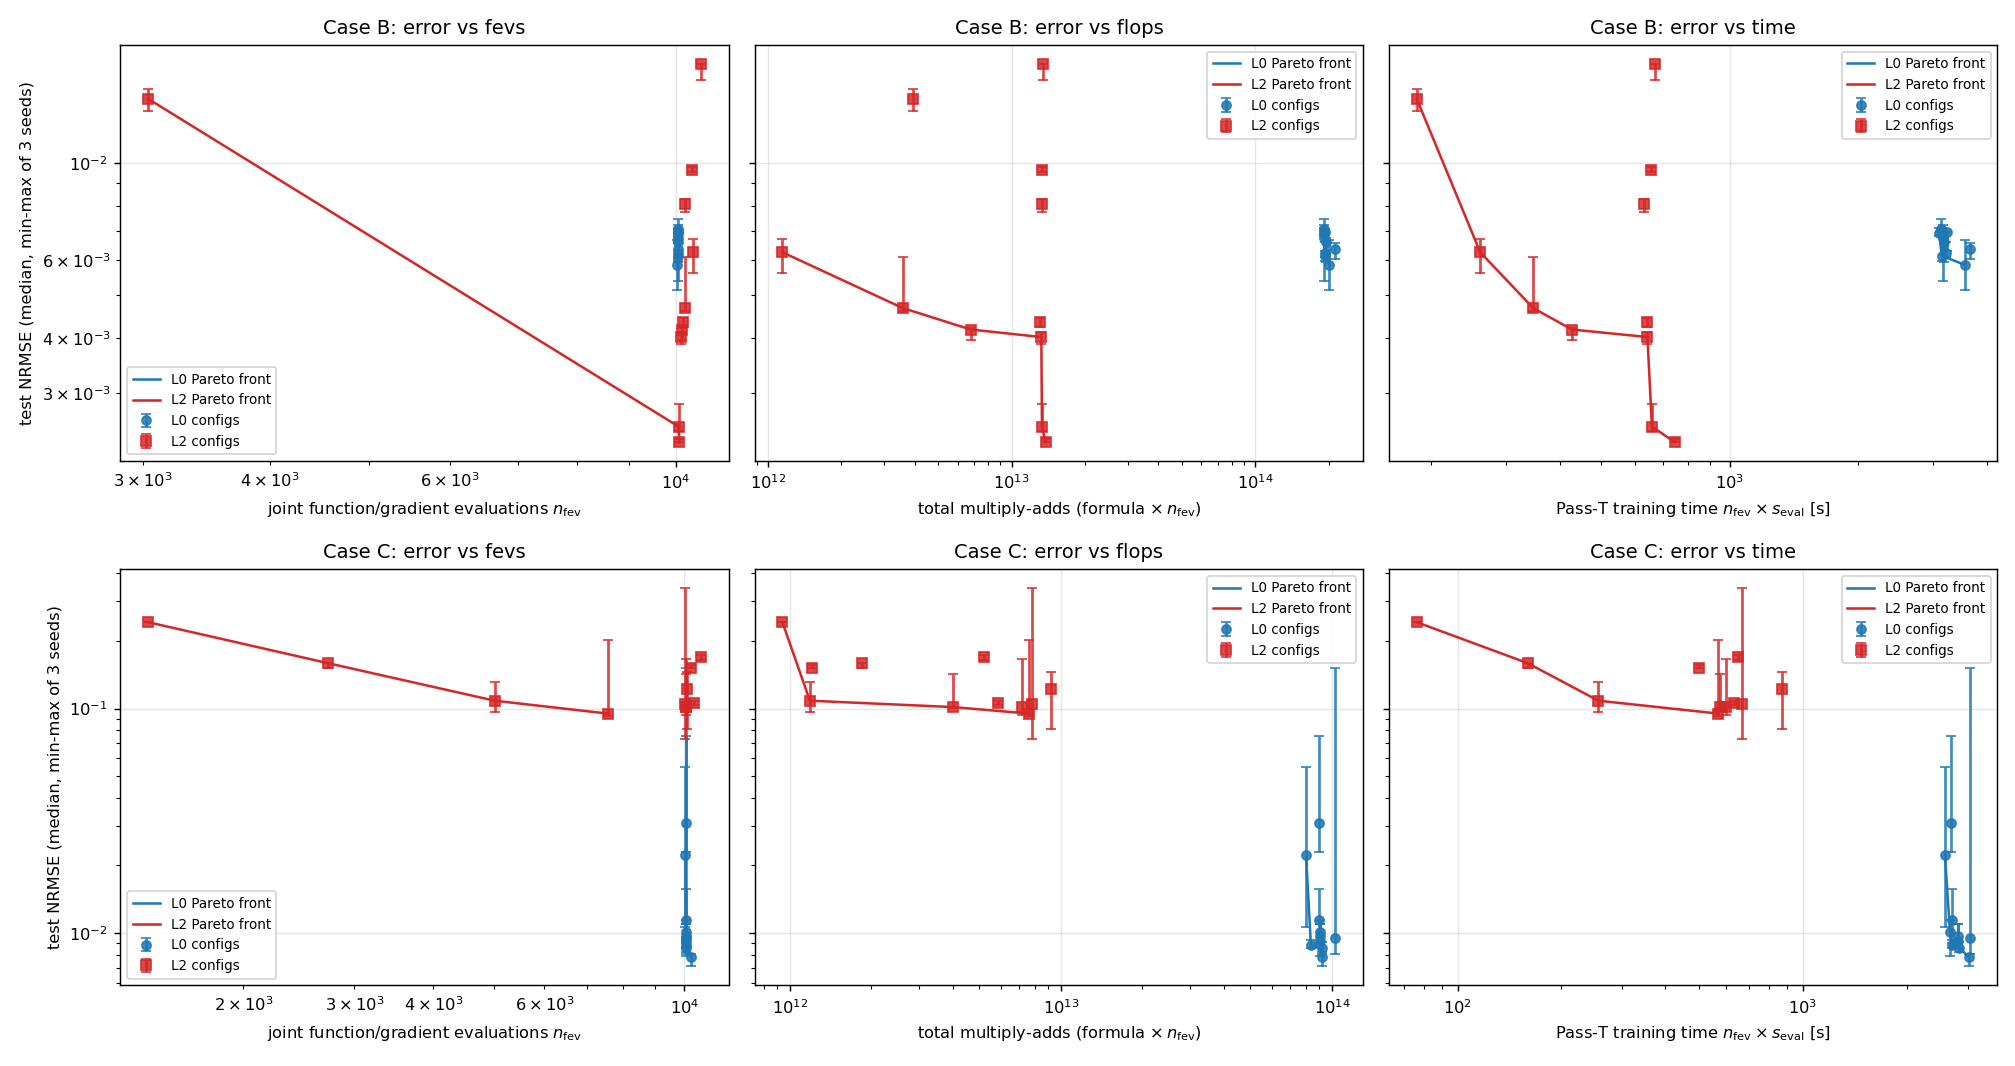
\includegraphics[width=0.90\textwidth,height=0.215\textheight,keepaspectratio]{fig3_cost_pareto.png}
  \caption{Final $10{,}000$-iteration cost-accuracy trade-offs and Pareto fronts for Case~B (\textbf{top row}) and Case~C (\textbf{bottom row}): test NRMSE (median and min--max range of 3 seeds) against function/gradient evaluations $n_{\mathrm{fev}}$ (\textbf{left}), total training operations $\FLOPs_{\mathrm{total}} = n_{\mathrm{fev}}\FLOPs_{\mathrm{eval}}$ (\textbf{centre}), and exclusive-node Pass-T training time $T_{\mathrm{Pass\,T}} = n_{\mathrm{fev}} s_{\mathrm{eval}}$ at 16 threads (\textbf{right}), for $\mathrm{L0}$ (blue circles) and $\mathrm{L2}$ (red squares).}
  \label{fig:rq2bis_fig3}
\end{figure}

\begin{figure}[!htbp]
  \centering
  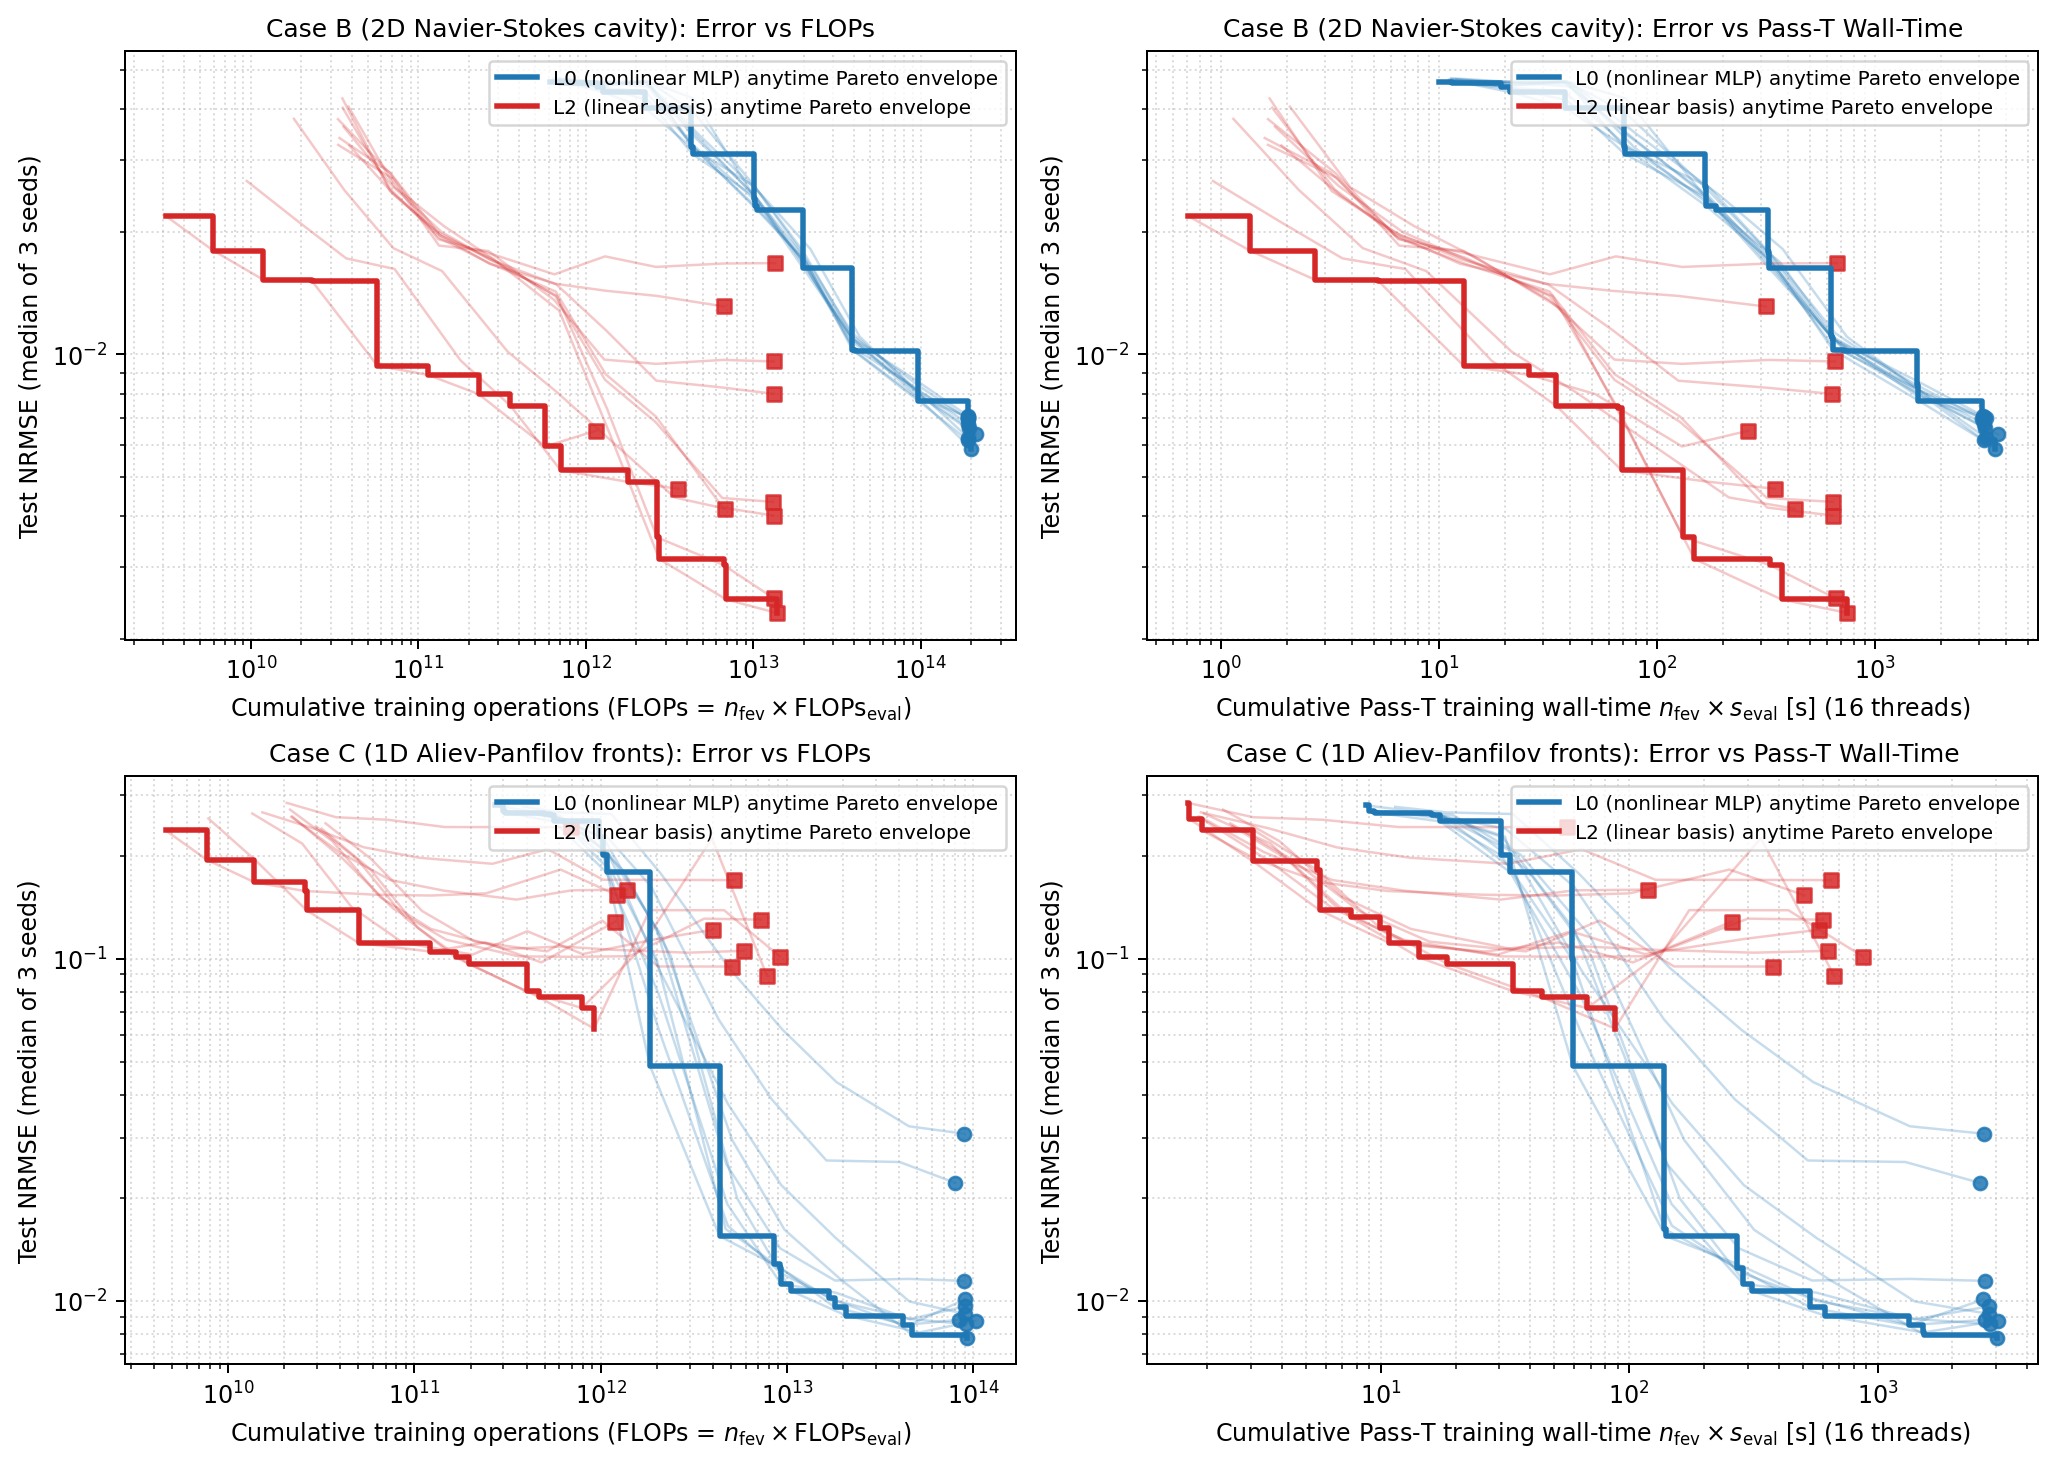
\includegraphics[width=0.90\textwidth,height=0.215\textheight,keepaspectratio]{fig_flops_trajectories.png}
  \caption{Continuous quasi-Newton optimization trajectories and anytime Pareto envelopes across all nine checkpoints $k \in \{25, 50, 100, 200, 500, 1000, 2000, 5000, 10000\}$ in the $(\FLOPs, \NRMSE)$ plane (\textbf{left column}) and $(T_{\mathrm{Pass\,T}}, \NRMSE)$ plane (\textbf{right column}) for Case~B (\textbf{top row}) and Case~C (\textbf{bottom row}). Thin translucent curves trace the 21 individual configurations (median of 3 seeds); bold step curves trace the anytime Pareto frontier of $\mathrm{L0}$ (blue) and $\mathrm{L2}$ (red).}
  \label{fig:flops_trajectories}
\end{figure}

Figure~\ref{fig:flops_trajectories} makes the computational scalability of both architectures transparent across the entire range of compute budgets from $3\cdot 10^9$ to $2\cdot 10^{14}$ FLOPs:
\begin{itemize}[leftmargin=2em]
  \item \textbf{In Case B (top row of Figure~\ref{fig:flops_trajectories}), the anytime Pareto envelope of $\mathrm{L2}$ lies strictly to the left of and below $\mathrm{L0}$ by $1.5$ to $2$ orders of magnitude in FLOPs and $1$ order of magnitude in wall-clock time at every accuracy level:} Before $\mathrm{L0}$ has completed even its first checkpoint at $k = 25$ iterations ($\sim 6.5\cdot 10^{11}$ FLOPs, $\sim 10.5$~s, where $\mathrm{L0}$ sits at $\NRMSE \approx 4.6\cdot 10^{-2}$), the $\mathrm{L2}$ envelope has already passed $\NRMSE = 9.0\cdot 10^{-3}$ at $10^{11}$ FLOPs ($\sim 13$~s) and $\NRMSE = 5.6\cdot 10^{-3}$ at $6\cdot 10^{11}$ FLOPs! Between $10^{10}$ and $10^{13}$ FLOPs, the $\mathrm{L2}$ anytime envelope decays according to an empirical compute scaling law
  \begin{equation}
    \NRMSE_{\mathrm{B, L2}}(\FLOPs) \propto \FLOPs^{-0.35},
  \end{equation}
  reducing error by roughly a factor of $2.2\times$ for every decade of FLOPs invested, until converging at $\NRMSE = 2.32\cdot 10^{-3}$ at $1.38\cdot 10^{13}$ FLOPs ($744$~s). By contrast, $\mathrm{L0}$ spans the decade $6\cdot 10^{11}$ to $2\cdot 10^{14}$ FLOPs ($10$~s to $3650$~s) and bottoms out at $5.86\cdot 10^{-3}$.
  \item \textbf{In Case C (bottom row of Figure~\ref{fig:flops_trajectories}), the $\mathrm{L2}$ and $\mathrm{L0}$ anytime envelopes cross sharply at $\FLOPs \approx 1.2\cdot 10^{12}$ ($T_{\mathrm{Pass\,T}} \approx 60$~s):} Below $10^{12}$ FLOPs (where $\mathrm{L0}$ has completed fewer than 100 BFGS iterations and still has $\NRMSE > 0.18$), $\mathrm{L2}$ provides a fast rough approximation down to $\NRMSE \approx 0.07$--$0.10$. At $\FLOPs \approx 1.2\cdot 10^{12}$ (iteration $200$--$500$ of $\mathrm{L0}$), the $\mathrm{L0}$ trajectory plunges nearly vertically through the Kolmogorov barrier---dropping from $0.20$ to $1.6\cdot 10^{-2}$ within half a decade of FLOPs---and continues down to $7.83\cdot 10^{-3}$ at $9.23\cdot 10^{13}$ FLOPs ($3024$~s), while $\mathrm{L2}$ curls upward due to high-iteration polynomial overfitting.
\end{itemize}

\subsection{Iso-Accuracy Compute Trade-Offs and Time-to-Target Speedups}

To quantify Hypothesis~H6 (\texttt{cost\_to\_reach}), Table~\ref{tab:cost_to_reach} reports the cheapest configuration (in total FLOPs and Pass-T wall-time at completion) of $\mathrm{L0}$ and $\mathrm{L2}$ that reaches target multiples $\{1.00\times, 1.25\times, 1.50\times, 2.00\times, 3.00\times\}$ of the best $\mathrm{L0}$ median test NRMSE, and Table~\ref{tab:time_to_target} reports the in-flight checkpoint \texttt{time\_to\_target} required to reach fixed validation NRMSE thresholds $\{0.05, 0.02, 0.01\}$.

\begin{table}[!htbp]
\centering
\caption{Hypothesis~H6 (\texttt{cost\_to\_reach}): cheapest completed configuration of $\mathrm{L0}$ and $\mathrm{L2}$ achieving target multiples of the best $\mathrm{L0}$ median test NRMSE ($5.86\cdot 10^{-3}$ in Case~B; $7.83\cdot 10^{-3}$ in Case~C), comparing total training operations $\FLOPs_{\mathrm{total}}$, exclusive-node Pass-T time $T_{\mathrm{Pass\,T}}$ (16 threads), and shared-node Pass-A time $T_{\mathrm{Pass\,A}}$.}
\label{tab:cost_to_reach}
\footnotesize\resizebox{\textwidth}{!}{%

\begin{tabular}{@{}llrlrrlrrrrr@{}}
\toprule
\textbf{Case} & \textbf{Level} & \textbf{Target} & \textbf{Cheapest L0} & \textbf{L0 FLOPs} & \textbf{L0 $T_{\mathrm{T}}$[s]} & \textbf{Cheapest L2} & \textbf{L2 FLOPs} & \textbf{L2 $T_{\mathrm{T}}$[s]} & $\frac{\text{FLOPs}_{\mathrm{L0}}}{\text{FLOPs}_{\mathrm{L2}}}$ & $\frac{T_{\mathrm{T,L0}}}{T_{\mathrm{T,L2}}}$ & $\frac{T_{\mathrm{A,L0}}}{T_{\mathrm{A,L2}}}$ \\
\midrule
\textbf{B}
 & $1.00\times$ & $5.86\cdot 10^{-3}$ & $w{=}7,L{=}2,n{=}5$ & $2.01\cdot 10^{14}$ & $3556$ & $K{=}17,w{=}7,n{=}10$ & $3.57\cdot 10^{12}$ & $347$ & $\mathbf{56.3\times}$ & $\mathbf{10.3\times}$ & $7.8\times$ \\
 & $1.25\times$ & $7.33\cdot 10^{-3}$ & $w{=}2,L{=}2,n{=}1$ & $1.92\cdot 10^{14}$ & $3090$ & $K{=}5,w{=}7,n{=}10$  & $1.15\cdot 10^{12}$ & $261$ & $\mathbf{167\times}$  & $\mathbf{11.9\times}$ & $7.7\times$ \\
 & $\mathbf{1.50\times}$ & $\mathbf{8.79\cdot 10^{-3}}$ & $w{=}2,L{=}2,n{=}1$ & $1.92\cdot 10^{14}$ & $3090$ & $K{=}5,w{=}7,n{=}10$  & $1.15\cdot 10^{12}$ & $261$ & $\mathbf{167\times}$  & $\mathbf{11.9\times}$ & $7.7\times$ \\
 & $2.00\times$ & $1.17\cdot 10^{-2}$ & $w{=}2,L{=}2,n{=}1$ & $1.92\cdot 10^{14}$ & $3090$ & $K{=}5,w{=}7,n{=}10$  & $1.15\cdot 10^{12}$ & $261$ & $\mathbf{167\times}$  & $\mathbf{11.9\times}$ & $7.7\times$ \\
 & $3.00\times$ & $1.76\cdot 10^{-2}$ & $w{=}2,L{=}2,n{=}1$ & $1.92\cdot 10^{14}$ & $3090$ & $K{=}65,w{=}2,n{=}10$ & $3.95\cdot 10^{12}$ & $185$ & $\mathbf{167\times}$  & $\mathbf{16.7\times}$ & $12.1\times$ \\
\midrule
\textbf{C}
 & $1.00\times$ & $7.83\cdot 10^{-3}$ & $w{=}8,L{=}3,n{=}12$ & $9.23\cdot 10^{13}$ & $3024$ & \multicolumn{3}{c}{\emph{Unreachable (best L2 is $9.49\cdot 10^{-2}$)}} & $\infty$ & $\infty$ & $\infty$ \\
 & $1.25\times$ & $9.78\cdot 10^{-3}$ & $w{=}8,L{=}1,n{=}6$  & $8.37\cdot 10^{13}$ & $2700$ & \multicolumn{3}{c}{\emph{Unreachable}} & $\infty$ & $\infty$ & $\infty$ \\
 & $\mathbf{1.50\times}$ & $\mathbf{1.17\cdot 10^{-2}}$ & $w{=}8,L{=}1,n{=}12$ & $8.37\cdot 10^{13}$ & $2667$ & \multicolumn{3}{c}{\emph{Unreachable}} & $\infty$ & $\infty$ & $\infty$ \\
 & $3.00\times$ & $2.35\cdot 10^{-2}$ & $w{=}8,L{=}1,n{=}3$  & $8.03\cdot 10^{13}$ & $2580$ & \multicolumn{3}{c}{\emph{Unreachable}} & $\infty$ & $\infty$ & $\infty$ \\
\bottomrule
\end{tabular}
}
\end{table}

\begin{table}[!htbp]
\centering
\caption{In-flight checkpoint \texttt{time\_to\_target}: function evaluations $n_{\mathrm{fev}}$, cumulative FLOPs, and Pass-T wall-time $T_{\mathrm{Pass\,T}}$ required to reach validation NRMSE thresholds $\{0.05, 0.02, 0.01\}$ on all $3/3$ seeds.}
\label{tab:time_to_target}
\footnotesize\resizebox{\textwidth}{!}{%

\begin{tabular}{@{}llrrrrrrrrr@{}}
\toprule
 & & \multicolumn{3}{c}{\textbf{Target $\NRMSE_{\mathrm{valid}} \le 0.05$}} & \multicolumn{3}{c}{\textbf{Target $\NRMSE_{\mathrm{valid}} \le 0.02$}} & \multicolumn{3}{c}{\textbf{Target $\NRMSE_{\mathrm{valid}} \le 0.01$}} \\
\cmidrule(lr){3-5}\cmidrule(lr){6-8}\cmidrule(lr){9-11}
\textbf{Case} & \textbf{Configuration} & $n_{\mathrm{fev}}$ & \textbf{FLOPs} & $T_{\mathrm{T}}$[s] & $n_{\mathrm{fev}}$ & \textbf{FLOPs} & $T_{\mathrm{T}}$[s] & $n_{\mathrm{fev}}$ & \textbf{FLOPs} & $T_{\mathrm{T}}$[s] \\
\midrule
\textbf{B}
 & L0 canonical ($w{=}7, L{=}2, n{=}1$)      & $32$ & $6.11\cdot 10^{11}$ & $10.0$  & $1050$ & $2.01\cdot 10^{13}$ & $328.0$ & $2050$ & $3.92\cdot 10^{13}$ & $641.0$ \\
 & L0 best ($w{=}7, L{=}2, n{=}5$)           & $32$ & $6.41\cdot 10^{11}$ & $11.3$  & $527$  & $1.06\cdot 10^{13}$ & $187.0$ & $2030$ & $4.07\cdot 10^{13}$ & $721.0$ \\
 & L2 low-mode ($K{=}5, w{=}7, n{=}10$)      & $28$ & $3.09\cdot 10^9$    & $\mathbf{0.70}$ & $31$   & $3.42\cdot 10^9$    & $\mathbf{0.78}$  & $516$  & $5.70\cdot 10^{10}$ & $\mathbf{12.9}$ \\
 & L2 mid-mode ($K{=}17, w{=}7, n{=}10$)     & $27$ & $9.45\cdot 10^9$    & $0.92$  & $52$   & $1.82\cdot 10^{10}$ & $1.77$  & $511$  & $1.79\cdot 10^{11}$ & $17.4$ \\
 & L2 canonical ($K{=}65, w{=}7, n{=}10$)    & $27$ & $3.53\cdot 10^{10}$ & $1.71$  & $57$   & $7.46\cdot 10^{10}$ & $3.62$  & $1010$ & $1.32\cdot 10^{12}$ & $63.9$ \\
 & L2 widest ($K{=}65, w{=}28, n{=}10$)      & $28$ & $3.83\cdot 10^{10}$ & $2.07$  & $103$  & $1.41\cdot 10^{11}$ & $7.60$  & $1010$ & $1.38\cdot 10^{12}$ & $74.3$ \\
\midrule
\textbf{C}
 & L0 canonical ($w{=}8, L{=}1, n{=}12$)     & $523$ & $4.69\cdot 10^{12}$ & $138.0$ & $523$  & $4.69\cdot 10^{12}$ & $138.0$ & $2030$ & $1.82\cdot 10^{13}$ & $537.0$ \\
 & L0 best-deep ($w{=}8, L{=}3, n{=}12$)     & $564$ & $5.08\cdot 10^{12}$ & $166.0$ & $1050$ & $9.46\cdot 10^{12}$ & $309.0$ & $5090$ & $4.59\cdot 10^{13}$ & $1500.0$ \\
 & L0 widest ($w{=}32, L{=}1, n{=}12$)       & $526$ & $4.82\cdot 10^{12}$ & $149.0$ & $526$  & $4.82\cdot 10^{12}$ & $149.0$ & $2040$ & $1.87\cdot 10^{13}$ & $576.0$ \\
 & L2 (all 11 configurations)                & \multicolumn{9}{c}{\emph{0/3 seeds reach $\le 0.05$, $\le 0.02$, or $\le 0.01$ at any checkpoint}} \\
\bottomrule
\end{tabular}
}
\end{table}

In Case~B, the in-flight checkpoint speedups (Table~\ref{tab:time_to_target}) are even larger than the end-of-run ratios because the fixed orthonormal POD basis acts as a strong preconditioner for the early quasi-Newton steps: to reach $\NRMSE_{\mathrm{valid}} \le 0.02$, $\mathrm{L2}$ ($K=5, w=7, n=10$) requires only $31$ evaluations ($3.42\cdot 10^9$ FLOPs, \textbf{$0.78$~seconds}), compared with $1050$ evaluations ($2.01\cdot 10^{13}$ FLOPs, \textbf{$328$~seconds}) for canonical $\mathrm{L0}$---a \textbf{$5870\times$ reduction in FLOPs} and a \textbf{$421\times$ reduction in wall-clock time}! To reach $\NRMSE_{\mathrm{valid}} \le 0.01$, $\mathrm{L2}$ ($K=5$) requires \textbf{$688\times$ fewer FLOPs} ($5.70\cdot 10^{10}$ vs.\ $3.92\cdot 10^{13}$) and \textbf{$50\times$ less wall-time} ($12.9$~s vs.\ $641$~s).

\subsection{Hardware Throughput, Arithmetic Intensity, and Why One \texorpdfstring{$\mathrm{L2}$}{L2} FLOP Costs \texorpdfstring{$3\times$}{3x} More Wall-Time Than One \texorpdfstring{$\mathrm{L0}$}{L0} FLOP}
\label{sec:flops_roofline}

A critical finding of Stage~5 (Pass~T) on the CINECA Leonardo supercomputer is that while $\mathrm{L2}$ reduces $\FLOPs_{\mathrm{eval}}$ by $14.6\times$ (at $K=65$) to $173\times$ (at $K=5$) in Case~B, the measured exclusive-node evaluation time $s_{\mathrm{eval}}$ at 16 threads decreases by \textbf{$4.9\times$} ($0.313$~s vs.\ $0.0635$~s at $K=65$) to \textbf{$12.5\times$} ($0.0251$~s at $K=5$). Why does an $\mathrm{L2}$ floating-point operation take $3.01\times$ (Case~B) to $3.08\times$ (Case~C) longer in wall-clock time than an $\mathrm{L0}$ floating-point operation?

Figures~\ref{fig:rq2bis_fig5} and~\ref{fig:flops_arithmetic} and Tables~\ref{tab:h2_cost_split} and~\ref{tab:thread_scaling} provide the complete hardware explanation via the Roofline performance model~\cite{williams2009roofline} and Amdahl's law.

\begin{figure}[!htbp]
  \centering
  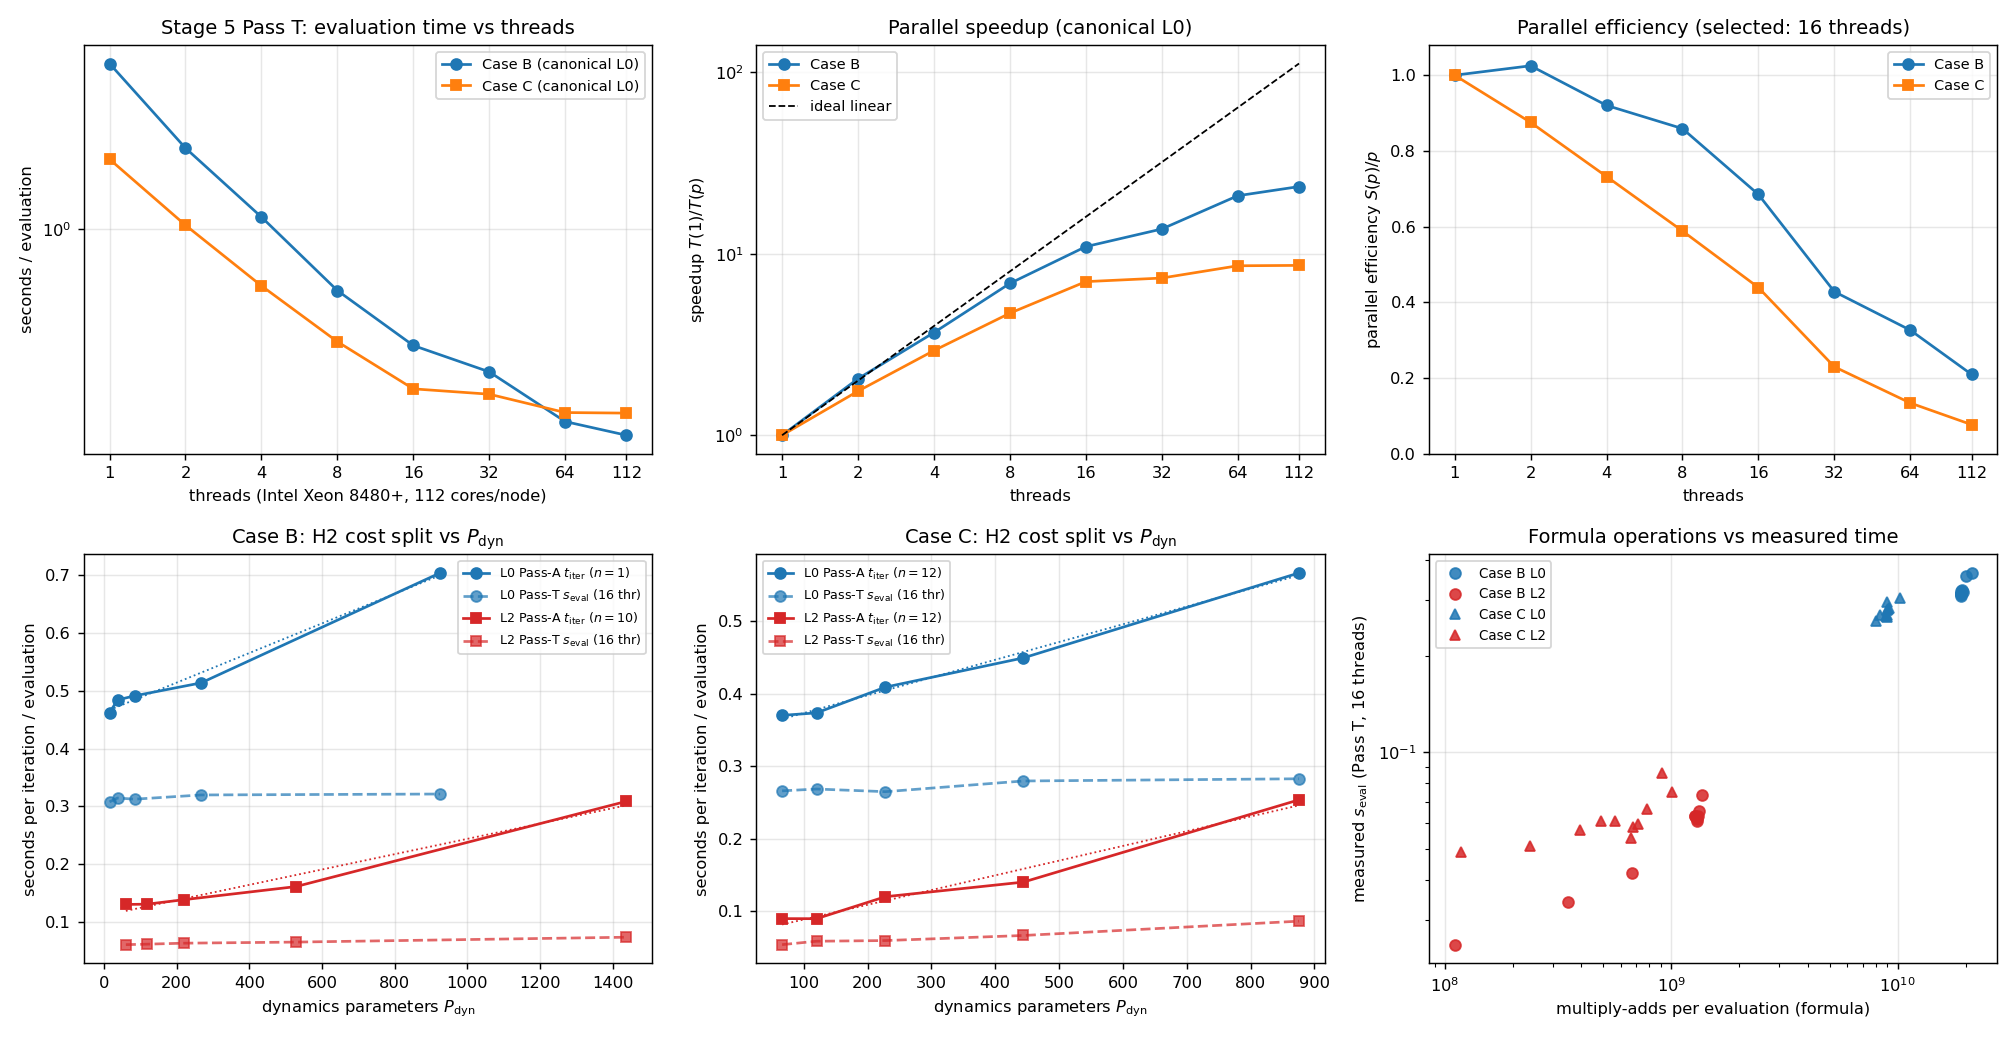
\includegraphics[width=0.90\textwidth,height=0.215\textheight,keepaspectratio]{fig5_timing_and_scaling.png}
  \caption{Stage~5 Pass-T hardware benchmarks on exclusive 112-core CINECA Leonardo DCGP nodes (dual-socket Intel Xeon Platinum 8480+). \textbf{Top row:} multi-core thread scaling $p \in \{1, 2, 4, 8, 16, 32, 64, 112\}$ of the canonical $\mathrm{L0}$ model---seconds per evaluation $s_{\mathrm{eval}}$ (left), parallel speedup $S(p) = T(1)/T(p)$ (centre), and parallel efficiency $E(p) = S(p)/p$ (right). \textbf{Bottom row:} H2 linear cost splits $t(P_{\mathrm{dyn}}) = t_0 + t_1 P_{\mathrm{dyn}}$ across the width sweeps of Case~B (left) and Case~C (centre), and measured $s_{\mathrm{eval}}$ against analytical $\FLOPs_{\mathrm{eval}}$ across all 42 configurations (right).}
  \label{fig:rq2bis_fig5}
\end{figure}

\begin{figure}[!htbp]
  \centering
  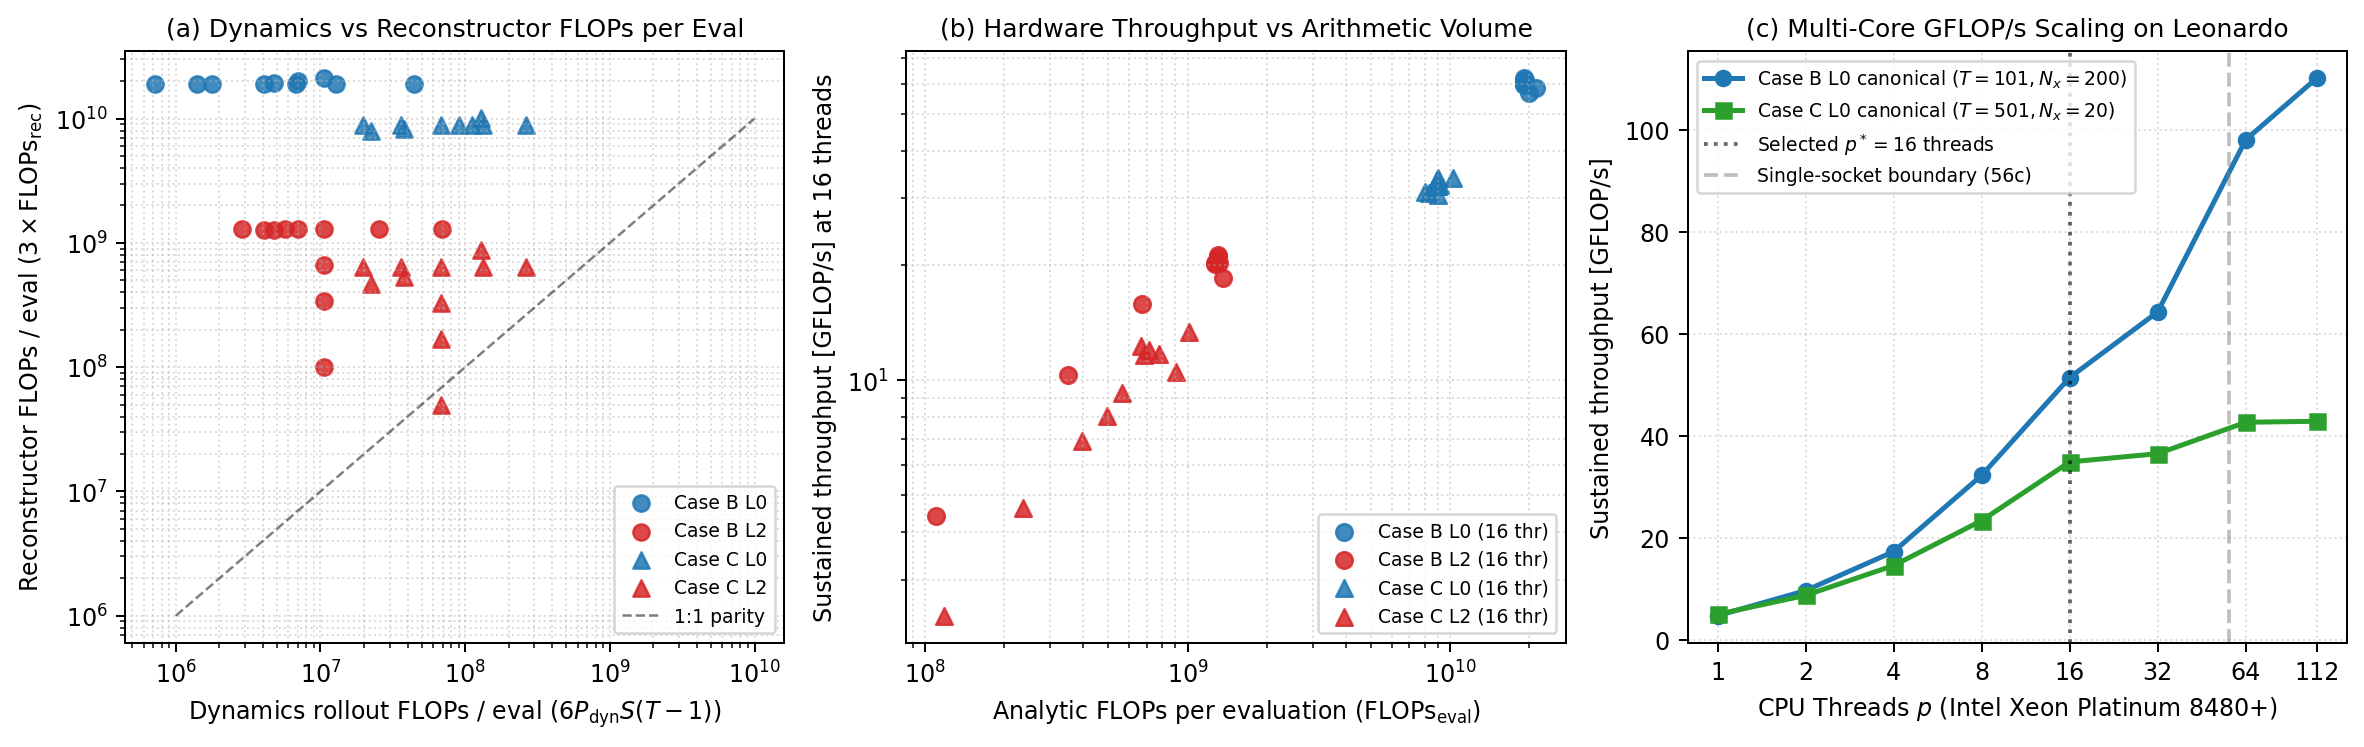
\includegraphics[width=0.90\textwidth,height=0.215\textheight,keepaspectratio]{fig_flops_arithmetic_intensity.png}
  \caption{Arithmetic structure and sustained hardware throughput (GFLOP/s) on CINECA Leonardo. \textbf{Panel (a):} decomposed dynamics rollout FLOPs ($6 P_{\mathrm{dyn}} S (N_t - 1)$) versus reconstructor FLOPs ($3\FLOPs_{\mathrm{rec}}^{\mathrm{fwd}}$) per evaluation across all 42 configurations, showing the 3-to-4 orders of magnitude separation in $\mathrm{L0}$ (blue) versus $\mathrm{L2}$ (red). \textbf{Panel (b):} sustained double-precision throughput ($\mathrm{GFLOP/s} = \FLOPs_{\mathrm{eval}} / s_{\mathrm{eval}} / 10^9$) at $p^* = 16$ threads as a function of arithmetic volume $\FLOPs_{\mathrm{eval}}$. \textbf{Panel (c):} multi-core sustained GFLOP/s scaling from $p=1$ to $p=112$ threads for Case~B ($N_t=101, N_x=200$, reaching $110.1$~GFLOP/s) and Case~C ($N_t=501, N_x=20$, saturating at $42.8$~GFLOP/s).}
  \label{fig:flops_arithmetic}
\end{figure}

\begin{table}[!htbp]
\centering
\caption{Hypothesis~H2 cost split: linear regression $t(P_{\mathrm{dyn}}) = t_0 + t_1 P_{\mathrm{dyn}}$ of per-iteration wall-time (Pass~A, 56-core shared node) and isolated evaluation time $s_{\mathrm{eval}}$ (Pass~T, 16 threads on exclusive node) across the dynamics width sweeps of Cases~B and~C.}
\label{tab:h2_cost_split}
\footnotesize\resizebox{\textwidth}{!}{%

\begin{tabular}{@{}lllrrrrl@{}}
\toprule
\textbf{Case} & \textbf{Arm} & \textbf{Timing Source} & \textbf{Intercept $t_0$ [s]} & \textbf{Slope $t_1$ [s/param]} & $\max P_{\mathrm{dyn}}$ ($4w^*$) & \textbf{Dyn.\ Share at $4w^*$} & \textbf{H2 Verdict ($< 50\%$)} \\
\midrule
\textbf{B} & L0 & Pass-T $s_{\mathrm{eval}}$ (excl.\ 16c) & $0.312$ & $1.13\cdot 10^{-5}$ & $925$  & $\mathbf{3.24\%}$  & \textbf{Supported} ($1.04\times$ max/min) \\
\textbf{B} & L0 & Pass-A $t_{\mathrm{iter}}$ (shared 56c) & $0.463$ & $2.56\cdot 10^{-4}$ & $925$  & $\mathbf{33.8\%}$  & \textbf{Supported} ($1.52\times$ max/min) \\
\textbf{B} & L2 & Pass-T $s_{\mathrm{eval}}$ (excl.\ 16c) & $0.0608$& $9.05\cdot 10^{-6}$ & $1438$ & $\mathbf{17.6\%}$  & \textbf{Supported} ($1.21\times$ max/min) \\
\textbf{B} & L2 & Pass-A $t_{\mathrm{iter}}$ (shared 56c) & $0.111$ & $1.33\cdot 10^{-4}$ & $1438$ & $\mathbf{63.1\%}$  & Falsified (L2 rec is $5\times$ cheaper) \\
\midrule
\textbf{C} & L0 & Pass-T $s_{\mathrm{eval}}$ (excl.\ 16c) & $0.264$ & $2.24\cdot 10^{-5}$ & $876$  & $\mathbf{6.90\%}$  & \textbf{Supported} ($1.06\times$ max/min) \\
\textbf{C} & L0 & Pass-A $t_{\mathrm{iter}}$ (shared 56c) & $0.349$ & $2.45\cdot 10^{-4}$ & $876$  & $\mathbf{38.1\%}$  & \textbf{Supported} ($1.53\times$ max/min) \\
\textbf{C} & L2 & Pass-T $s_{\mathrm{eval}}$ (excl.\ 16c) & $0.0517$& $3.83\cdot 10^{-5}$ & $876$  & $\mathbf{39.4\%}$  & \textbf{Supported} ($1.60\times$ max/min) \\
\textbf{C} & L2 & Pass-A $t_{\mathrm{iter}}$ (shared 56c) & $0.0683$& $2.03\cdot 10^{-4}$ & $876$  & $\mathbf{72.2\%}$  & Falsified (L2 rec is $5\times$ cheaper) \\
\bottomrule
\end{tabular}
}
\end{table}

\begin{table}[!htbp]
\centering
\caption{Stage~5 Pass-T strong thread scaling on an exclusive 112-core Intel Xeon Platinum 8480+ node (canonical $\mathrm{L0}$ configuration of Case~B on \texttt{lrdn4887} and Case~C on \texttt{lrdn4960}).}
\label{tab:thread_scaling}
\footnotesize\resizebox{\textwidth}{!}{%

\begin{tabular}{@{}rrrrrrrrr@{}}
\toprule
 & \multicolumn{4}{c}{\textbf{Case B ($\mathrm{L0}$, $N_t=101, N_x=200$, $1.911\cdot 10^{10}$ FLOPs/eval)}} & \multicolumn{4}{c}{\textbf{Case C ($\mathrm{L0}$, $N_t=501, N_x=20$, $8.966\cdot 10^9$ FLOPs/eval)}} \\
\cmidrule(lr){2-5}\cmidrule(lr){6-9}
\textbf{Threads $p$} & $s_{\mathrm{eval}}$ [s] & \textbf{Speedup $S(p)$} & \textbf{Eff.\ $E(p)$} & \textbf{GFLOP/s} & $s_{\mathrm{eval}}$ [s] & \textbf{Speedup $S(p)$} & \textbf{Eff.\ $E(p)$} & \textbf{GFLOP/s} \\
\midrule
$1$   & $4.075$ & $1.00\times$  & $100.0\%$ & $4.69$   & $1.809$ & $1.00\times$ & $100.0\%$ & $4.96$  \\
$2$   & $1.988$ & $2.05\times$  & $102.5\%$ & $9.61$   & $1.033$ & $1.75\times$ & $87.6\%$  & $8.68$  \\
$4$   & $1.107$ & $3.68\times$  & $92.0\%$  & $17.26$  & $0.617$ & $2.93\times$ & $73.3\%$  & $14.52$ \\
$8$   & $0.593$ & $6.87\times$  & $85.9\%$  & $32.22$  & $0.384$ & $4.71\times$ & $58.9\%$  & $23.34$ \\
$\mathbf{16}$ \emph{(selected)} & $\mathbf{0.372}$ & $\mathbf{10.96\times}$ & $\mathbf{68.5\%}$ & $\mathbf{51.39}$ & $\mathbf{0.257}$ & $\mathbf{7.03\times}$ & $\mathbf{43.9\%}$ & $\mathbf{34.85}$ \\
$32$  & $0.297$ & $13.71\times$ & $42.8\%$  & $64.26$  & $0.246$ & $7.36\times$ & $23.0\%$  & $36.46$ \\
$64$ \emph{(2 sockets)} & $0.195$ & $20.91\times$ & $32.7\%$  & $98.03$  & $0.210$ & $8.60\times$ & $13.4\%$  & $42.61$ \\
$112$ \emph{(full node)}& $0.174$ & $23.49\times$ & $21.0\%$  & $110.12$ & $0.209$ & $8.64\times$ & $7.7\%$   & $42.82$ \\
\bottomrule
\end{tabular}
}
\end{table}

Look at Panel~(b) of Figure~\ref{fig:flops_arithmetic} and Table~\ref{tab:flops_breakdown}:
\begin{enumerate}[leftmargin=2em]
  \item \textbf{High-throughput compute-bound regime of $\mathrm{L0}$ ($32$--$62$~GFLOP/s at 16 threads):} In $\mathrm{L0}$, $99.2\%$ to $99.98\%$ of the arithmetic consists of evaluating a 4- or 5-layer dense MLP on a flattened batch of $S \cdot N_t \cdot N_x = 1.616\cdot 10^6$ rows (Case~B, width $24$) or $1.002\cdot 10^6$ rows (Case~C, width $17$). These large, contiguous matrix-matrix multiplications (\texttt{GEMM}) saturate the AVX-512 vector units and L2/L3 caches of the Intel Xeon Platinum 8480+ processor across all 16 threads, achieving a sustained double-precision throughput of \textbf{$60.86$~GFLOP/s} ($1.64\cdot 10^{-11}$~s/op) in Case~B and \textbf{$32.36$~GFLOP/s} ($3.09\cdot 10^{-11}$~s/op) in Case~C.
  \item \textbf{Latency- and dispatch-bound regime of $\mathrm{L2}$ ($2.4$--$21.3$~GFLOP/s at 16 threads):} When $\mathrm{L0}$ is replaced by $\mathrm{L2}$, the massive spatial MLP batch vanishes. What remains is a single modal matrix product plus $N_t - 1$ \textbf{sequential Forward Euler steps} (\texttt{for i in tf.range(T - 1)}), each multiplying tiny matrices of shape $(S, w) = (80, 7)$ in Case~B or $(100, 8)$ in Case~C. A $(100 \times 8) \times (8 \times 12)$ matrix multiplication performs only $19{,}200$ FLOPs---far too small to amortize thread-pool fork/join synchronisation and TensorFlow kernel-dispatch overhead across 16 CPU cores! This serial time-loop overhead creates the irreducible intercept $t_0 \approx 0.052$--$0.061$~s in Table~\ref{tab:h2_cost_split}: at $K=65$, $\mathrm{L2}$ sustains $20.24$~GFLOP/s in Case~B ($4.94\cdot 10^{-11}$~s/op, $3.01\times$ slower per FLOP than $\mathrm{L0}$) and $10.52$~GFLOP/s in Case~C ($9.51\cdot 10^{-11}$~s/op, $3.08\times$ slower per FLOP than $\mathrm{L0}$); at $K=5$, where total FLOPs drop to $\sim 1.1\cdot 10^8$ while the sequential loop time remains fixed at $\sim 0.025$--$0.049$~s, sustained throughput falls to $4.40$~GFLOP/s (Case~B) and $2.41$~GFLOP/s (Case~C).
  \item \textbf{Amdahl's law in multi-core strong scaling ($p = 1 \to 112$ threads, Figure~\ref{fig:flops_arithmetic}c and Table~\ref{tab:thread_scaling}):} The exact same serial Forward Euler loop governs multi-core strong scaling across the 112 cores of the dual-socket Xeon node. Fitting Amdahl's law $S(p) = \big(f_{\mathrm{serial}} + (1 - f_{\mathrm{serial}})/p\big)^{-1}$ to Table~\ref{tab:thread_scaling} yields an effective serial fraction of \textbf{$f_{\mathrm{serial}} \approx 3.4\%$ in Case~B} ($N_t - 1 = 100$ Euler steps, $N_x = 200$ points/step, allowing speedup to reach $10.96\times$ at 16 threads and $23.49\times$ / $110.1$~GFLOP/s at 112 threads) versus \textbf{$f_{\mathrm{serial}} \approx 10.8\%$ in Case~C} ($N_t - 1 = 500$ Euler steps, $N_x = 20$ points/step---a $5\times$ longer sequential loop and $10\times$ smaller spatial batch per step---which caps speedup at $7.03\times$ at 16 threads and $8.64\times$ / $42.8$~GFLOP/s at 112 threads).
  \item \textbf{Why Pass-A slopes exceed Pass-T slopes (the dense BFGS inverse-Hessian update):} In Table~\ref{tab:h2_cost_split}, widening $\NNdyn$ from $w=2$ to $4w^*$ increases the isolated Pass-T evaluation time $s_{\mathrm{eval}}$ by only \textbf{$4.4\%$ in Case~B $\mathrm{L0}$} (dynamics share $3.24\%$) and \textbf{$6.3\%$ in Case~C $\mathrm{L0}$} (dynamics share $6.90\%$), confirming Hypothesis~H2 cleanly. In Pass-A per-iteration wall-time on a shared 56-core node, the widest $\mathrm{L0}$ takes $1.52\times$--$1.53\times$ longer than the narrowest (dynamics share $33.8\%$ and $38.1\%$, still $< 50\%$), because \texttt{scipy.optimize.minimize(method='BFGS')} updates a dense $P_{\mathrm{total}} \times P_{\mathrm{total}}$ inverse-Hessian matrix $H_k$ via two outer products at every iteration ($O(P_{\mathrm{total}}^2)$ overhead outside the TensorFlow evaluation) and experiences cross-shard memory-bandwidth contention on shared nodes.
\end{enumerate}

\section{Synthesis and Guidelines for the NMPDE and SciML Community}
\label{sec:discussion}

\subsection{Complete Hypotheses Scorecards (\texttt{RQ2} and \texttt{RQ2-bis})}

Tables~\ref{tab:scorecard_rq2} and~\ref{tab:scorecard_rq2bis} consolidate the formal falsification criteria, empirical evidence, and verdicts for the four hypotheses of \texttt{RQ2} and the six hypotheses of \texttt{RQ2-bis}.

\begin{table}[!htbp]
\centering
\caption{Scorecard of the four hypotheses of Part~I (\texttt{RQ2}: reconstructor nonlinearity ablation across 816 runs).}
\label{tab:scorecard_rq2}
\footnotesize\resizebox{\textwidth}{!}{%

\begin{tabular}{@{}p{2.2cm}p{4.3cm}p{5.5cm}p{3.2cm}@{}}
\toprule
\textbf{Hypothesis} & \textbf{Protocol Criterion} & \textbf{Empirical Evidence} & \textbf{Verdict} \\
\midrule
\textbf{RQ2-H1} \newline (Case A linear match) & Affine modal decoder $\mathrm{L2}$ with $K \le 5$ Fourier modes matches $\mathrm{L0}$; falsified if $\NRMSE_{\mathrm{L2}} > 1.5\,\NRMSE_{\mathrm{L0}}$ & \textbf{End-to-end (R2):} $\NRMSE_{\mathrm{L2}}/\NRMSE_{\mathrm{L0}} \in [0.44, 0.71]$ across all pairs with $d_s \in \{2,3,5\}$ and $K \in \{3,5\}$ (best $0.43\times$ at $d_s=3, K=5$). \textbf{Frozen latents (R1):} ratio in $[3.87, 5.22]$ because $\mathrm{L0}$ latents are cubically sheared ($R^2_{\mathrm{lin}} = 0.55$). & \textbf{Supported in R2}; falsified in R1 (proving $\mathrm{L0}$ latents are curved). \\
\midrule
\textbf{RQ2-H2} \newline (Case C front barrier) & Linear variants follow $\varepsilon_{\mathrm{proj}}(K)$ which decays slowly; $\mathrm{L3}$ does not close the gap; only $\mathrm{L0}$ does; falsified if $\NRMSE_{\mathrm{L3}}(K{=}65) \le 2\,\NRMSE_{\mathrm{L0}}$ & At $K=33$ (largest run in \texttt{RQ2}), $\mathrm{L3}/\mathrm{L0} = 3.16$ $[2.39, 3.93]$ at $d_s=12$, $4.71$ at $d_s=5$, $6.43$ at $d_s=3$; $\mathrm{L2}/\mathrm{L0} \ge 4.57$ (and $12.1\times$ at $K=65$ in \texttt{RQ2-bis}). Correction to clause 1: $\mathrm{L2}$ follows $\varepsilon_{\mathrm{proj}}(K)$ only for $K \lesssim d_s$ and then stalls at $\varepsilon_{\mathrm{rank}}(d_s)$. & \textbf{Supported} (with the rank-bound refinement for $\mathrm{L2}$). \\
\midrule
\textbf{RQ2-H3} \newline (Case B POD \& direction) & POD variants capture the bulk vortex flow; direction error near corners and weak vortices dominates; time extrapolation open in sign & POD decoders reach $4.4\cdot 10^{-3}$ ($\mathrm{L3}$) and $8.1\cdot 10^{-3}$ ($\mathrm{L2}$) in \texttt{RQ2}, and $2.32\cdot 10^{-3}$ ($\mathrm{L2}$) in \texttt{RQ2-bis}. $77\%$--$90\%$ of direction error comes from the $22\%$ of points with speed $< 0.1$ (quiescent bottom corners and vortex core, not upper lid corners). Extrapolation ratio $\varepsilon_{[20,40]}/\varepsilon_{[0,20]} \in [0.58, 1.07]$: no degradation. & \textbf{Supported} (with precision that quiescent lower corners dominate direction error). \\
\midrule
\textbf{RQ2-H4} \newline (Modality of $\mathrm{L0}$ latents) & If R1 is much worse than R2 for the same linear decoder ($\NRMSE_{\mathrm{R1}} > 2\,\NRMSE_{\mathrm{R2}}$ at equal $K$), $\mathrm{L0}$ latents are not modal by themselves & For $\mathrm{L2}$: R1/R2 is $10.75$ in Case~A (median $7.35$, $> 2$ in $75\%$ of configs), $2.08$ at best R2 in Case~B (median $1.63$), and $1.94$ in Case~C (where both R1 and R2 hit the rank bound). For $\mathrm{L1}$: R1/R2 is $8.98$ (A), $5.92$ (B), $2.99$ (C). For $\mathrm{L3}$: R1/R2 $\approx 0.94$--$1.12$ everywhere. & \textbf{Supported in A and B} (and by $\mathrm{L1}$ in C); $\mathrm{L3}$ confirms information completeness. \\
\bottomrule
\end{tabular}
}
\end{table}

\begin{table}[!htbp]
\centering
\caption{Scorecard of the six hypotheses of Part~II (\texttt{RQ2-bis}: computational scalability at $10{,}000$ BFGS iterations on CINECA Leonardo).}
\label{tab:scorecard_rq2bis}
\footnotesize\resizebox{\textwidth}{!}{%

\begin{tabular}{@{}p{2.2cm}p{4.1cm}p{5.7cm}p{3.2cm}@{}}
\toprule
\textbf{Hypothesis} & \textbf{Protocol Criterion} & \textbf{Empirical Evidence at $10{,}000$ BFGS Iterations} & \textbf{Verdict} \\
\midrule
\textbf{RQ2bis-H1} \newline (Capacity power law) & Test NRMSE decreases as $E_\infty + a P_{\mathrm{dyn}}^{-\alpha}$ then plateaus; falsified if flat from $w_{\min}$ or 95\% CI of $\alpha$ reaches $< 0.1$ & \textbf{B L0 ($n{=}1$):} flat ($6.94\to 6.15\to 6.98\cdot 10^{-3}$), $\alpha=0.12$ CI $[0.00, 2.53]$. \textbf{B L2 ($n{=}10$):} $1.40\cdot 10^{-2}\to 2.32\cdot 10^{-3}$, $\alpha=1.11$ CI $[1.04, 1.23]$. \textbf{C L0 ($n{=}12$):} $3.08\cdot 10^{-2}\to 8.57\cdot 10^{-3}$, $\alpha=3.22$ CI $[1.88, 4.77]$. \textbf{C L2 ($n{=}12$):} stalls/overfits around $0.10$, $\alpha=1.77$ CI $[0.03, 1.80]$. & \textbf{Holds when reconstructor is not the bottleneck (B L2, C L0); falsified when it is (B L0, C L2).} \\
\midrule
\textbf{RQ2bis-H2} \newline (Cost split) & Widening $\NNdyn$ is cheap relative to $\NNrec$; falsified if dynamics share of per-iteration time at $4w^*$ exceeds $50\%$ & \textbf{Pass-T isolated eval (16 threads):} share at $4w^*$ is $\mathbf{3.2\%}$ (B L0), $\mathbf{6.9\%}$ (C L0), $\mathbf{17.6\%}$ (B L2), $\mathbf{39.4\%}$ (C L2) --- all $< 50\%$. \textbf{Pass-A shared-node time:} $33.8\%$ (B L0), $38.1\%$ (C L0) $< 50\%$; $63.1\%$ (B L2), $72.2\%$ (C L2) $> 50\%$ because $\mathrm{L2}$ cuts $\NNrec$ cost by $5\times$. & \textbf{Supported for L0 (Pass T \& A) and L2 (Pass T)}; falsified for L2 Pass A only because $\mathrm{L2}$ is so fast. \\
\midrule
\textbf{RQ2bis-H3} \newline (Iteration-limited regime) & Under a fixed iteration cap, large networks are under-converged so error vs.\ width is non-monotone or flattens at $I_{\max}$ & \textbf{At $1{,}000$ iters:} non-monotone in B L0, C L0, C L2. \textbf{At $10{,}000$ iters:} \textbf{B L0} remains non-monotone ($w=28$ at $6.98\cdot 10^{-3}$ vs.\ $w=7$ at $6.15\cdot 10^{-3}$); \textbf{C L0} and \textbf{B L2} have converged and are strictly monotone decreasing; \textbf{C L2} overfits at $w=16,32$. & \textbf{Supported at $1{,}000$ iters and for B L0 at $10{,}000$}; falsified for C L0 and B L2 once given $10{,}000$ iters. \\
\midrule
\textbf{RQ2bis-H4} \newline (Latent dimension) & Error stops improving once $n$ exceeds intrinsic dimension; falsified if improvement from $n^*$ to $2n^*$ is $\ge 5\%$ & \textbf{B L0 ($1\to 2$):} $-7.4\%$. \textbf{B L2 ($1\to 2$):} $\mathbf{+42.7\%}$ (and $+54.8\%$ from $2\to 5$). \textbf{C L0 ($12\to 24$):} $+6.1\%$ test, $+4.8\%$ valid (best is $n=6$ at $8.82\cdot 10^{-3}$). \textbf{C L2 ($12\to 24$):} $+6.6\%$ test, $+0.9\%$ valid (capped at rank $w^*=8$ by Prop.~\ref{prop:dyn_rank_bound}). & \textbf{Supported for B L0; falsified for B L2} (linear rank bound requires $n \ge 10$); borderline in C. \\
\midrule
\textbf{RQ2bis-H5} \newline (No free lunch in wall-time) & Lowest-error config is not the largest one ($\max P_{\mathrm{total}}$) & \textbf{B L0:} best is $w=7, n=5$ ($P=2211$), not $w=28$ ($P=2895$). \textbf{C L0:} best is $w=8, L=3$ ($P=1852$), not $w=32$ ($P=2356$). \textbf{B L2:} largest ($w=28, n=10, P=2218$) is best ($2.32\cdot 10^{-3}$). & \textbf{Supported for L0 in both cases; falsified for B L2} where BFGS converges cleanly up to $w=28$. \\
\midrule
\textbf{RQ2bis-H6} \newline (Compute value of linear arm) & $\mathrm{L2}$ reaches $1.5\times$ best $\mathrm{L0}$ median test NRMSE at lower operations and Pass-T time than $\mathrm{L0}$ & \textbf{Case B ($1.5\times$ target $= 8.79\cdot 10^{-3}$):} $\mathrm{L2}$ ($K=5, w=7, n=10$) uses $\mathbf{167\times}$ \textbf{fewer FLOPs} and $\mathbf{11.9\times}$ \textbf{less Pass-T time} ($261$~s vs.\ $3090$~s); at $1.0\times$ target ($5.86\cdot 10^{-3}$), $\mathbf{56.3\times}$ fewer FLOPs and $\mathbf{10.3\times}$ less time. \textbf{Case C:} unreachable by $\mathrm{L2}$ at any cost. & \textbf{Strongly supported in Case B; falsified in Case C.} \\
\bottomrule
\end{tabular}
}
\end{table}

\subsection{Practical Architectural Guidelines for Scientific Machine Learning}

Combining the mathematical bounds of Section~\ref{sec:math} with the 942 cluster and workstation runs of Sections~\ref{sec:rq2}--\ref{sec:flops} yields seven concrete guidelines for researchers designing latent dynamical models and neural operators for PDEs:

\begin{enumerate}[leftmargin=2em]
  \item \textbf{Diagnose the Kolmogorov $n$-width decay before choosing between an implicit MLP ($\mathrm{L0}$) and a linear modal reconstructor ($\mathrm{L2}$):} Compute the singular values $\sigma_k/\sigma_1$ of the centred training snapshots and the projection floor $\varepsilon_{\mathrm{proj}}(K)$ before any network training (Section~\ref{sec:spectra_and_floors}). If $\varepsilon_{\mathrm{proj}}(K)$ reaches the target accuracy within $K \lesssim 30$--$65$ modes (as in elliptic, parabolic, or viscous incompressible vortex flows such as Cases~A and~B), replace the pointwise MLP $\NNrec(\mathbf{z},\mathbf{x})$ with the affine POD/spectral expansion $\mathrm{L2}$. At full quasi-Newton convergence, $\mathrm{L2}$ is not merely a fast approximation to $\mathrm{L0}$---it achieves $2.5\times$ lower field error, $4.7\times$ lower vorticity error, $9.5\times$ lower direction error, $56\times$--$167\times$ lower training FLOPs, $10\times$ shorter training wall-time, $67\times$--$111\times$ faster inference, and exact preservation of linear physical constraints such as $\nabla\cdot\mathbf{v} = 0$. Conversely, if $\sigma_k/\sigma_1$ decays slowly due to sharp moving fronts or shocks (Case~C), retain the non-separable pointwise MLP $\mathrm{L0}$.
  \item \textbf{Always enforce the structural coupling rule $w_{\mathrm{dyn}} \ge n$ (Proposition~\ref{prop:dyn_rank_bound}):} Never increase the latent dimension $n$ above the hidden width $w_{\mathrm{dyn}}$ of the last hidden layer of $\NNdyn$. Because Forward Euler increments from $\mathbf{s}(0) = \mathbf{0}$ lie in $\operatorname{range}(W_{\mathrm{out}}) + \operatorname{span}\{\mathbf{b}_{\mathrm{out}}\}$ (and strictly in $\operatorname{range}(W_{\mathrm{out}})$ under rest-state equilibrium subtraction), any latent dimension beyond $w_{\mathrm{dyn}} + 1$ (or $w_{\mathrm{dyn}}$) has zero singular values up to floating-point round-off ($\sim 10^{-16}$). When using a linear reconstructor $\mathrm{L2}$, select $n$ from the POD rank floor $\varepsilon_{\mathrm{rank}}(n)$ first, and then set $w_{\mathrm{dyn}} \ge 2n$.
  \item \textbf{Scale $\NNdyn$ depth rather than width when modelling stiff fast--slow reaction kinetics with $\mathrm{L0}$:} Because $\NNdyn$ accounts for less than $0.3\%$ (Case~B) to $2.9\%$ (Case~C) of the FLOPs of an $\mathrm{L0}$ evaluation and less than $7\%$ of isolated multi-core evaluation wall-time, adding capacity to $\NNdyn$ is computationally almost free. In Case~C $\mathrm{L0}$, increasing hidden depth from $L=1$ to $L=3$ at $w^*=8$ ($P_{\mathrm{dyn}} = 372$) achieved the lowest error of the entire study ($7.83\cdot 10^{-3}$, front arrival MAE $0.54$~ms), outperforming a single hidden layer of width $w=32$ ($P_{\mathrm{dyn}} = 876$, $8.57\cdot 10^{-3}$) at less than half the parameter count.
  \item \textbf{Do not benchmark implicit neural reconstructors ($\mathrm{L0}$) at $500$--$1{,}000$ BFGS iterations:} Pure BFGS without Adam warm-up converges reliably on LDNets (0 NaN divergences across all 126 cluster runs), but builds curvature information over $O(P_{\mathrm{total}}) \sim 2{,}000$--$10{,}000$ iterations. Stopping at $500$ or $1{,}000$ iterations cuts every convergent $\mathrm{L0}$ and wide $\mathrm{L2}$ trajectory mid-descent, leaving $55\%$ to $66\%$ of the error reduction on the table and measuring early Hessian preconditioning rather than asymptotic model capacity.
  \item \textbf{When using a high-degree polynomial basis ($\mathrm{L2}$), ensure the spatial training subsample satisfies $N_x \ge K$:} In Case~C $\mathrm{L2}$, evaluating $K = 65$ Legendre modes on only $N_x = 20$ random spatial points per time step allowed wide dynamics networks ($w = 16, 32$) to overfit degree-64 polynomial oscillations between the 20 training points after iteration $1{,}000$. Because modal synthesis on 101 grid points is a tiny matrix multiplication, training $\mathrm{L2}$ on all $N_h = 101$ grid points costs negligible extra FLOPs and eliminates subsampling aliasing completely.
  \item \textbf{Always include a trainable modal offset $\mathbf{b}$ when centring snapshots around $\bar{y}(\mathbf{x})$:} If $\bar{y}(\mathbf{x}) \ne 0$ and the latent state starts at $\mathbf{s}(0) = \mathbf{0}$, a parameter-free modal identity ($\mathrm{L1}$) predicts $\hat{y}(\cdot,0) = \bar{y}$ instead of the rest state, generating an initial-condition shock that accounts for $54\%$ of $\mathrm{L1}$'s total squared error in Case~A.
  \item \textbf{Compile or fuse the sequential Forward Euler loop to convert $\mathrm{L2}$'s $15\times$--$167\times$ FLOP advantage into full wall-clock speedup:} On modern multi-core CPUs, $\mathrm{L2}$'s per-evaluation wall-time is floored at $t_0 \approx 0.05$--$0.06$~s by Python/TensorFlow dispatch over $N_t - 1$ sequential Euler steps of tiny $(S, w)$ matrices. Compiling the time-stepping rollout into a single fused kernel (via XLA \texttt{tf.function(jit\_compile=True)} or a custom C++/CUDA scan kernel) will eliminate per-step dispatch latency and bring wall-time speedups much closer to the analytical FLOP ratios.
\end{enumerate}

\subsection{Limitations and Threats to Validity}
\label{sec:rq2_limitations}

In accordance with rigorous empirical standards in numerical analysis and scientific computing, we document the main limitations and threats to validity of our two campaigns:
\begin{enumerate}[leftmargin=2em]
  \item \textbf{Cross-node AVX-512 floating-point non-determinism on the cluster:} In the CINECA Leonardo campaign, Stage~0 (canonical $\mathrm{L0}$) was executed across all four Slurm array shards on four distinct physical compute nodes (\texttt{results\_shard0..3/}). Even with \texttt{tf.config.experimental.enable\_op\_determinism()} enabled and identical random seeds, multi-threaded AVX-512 reductions across different physical nodes introduce $\sim 10^{-16}$ rounding variations in the initial gradients, which quasi-Newton inverse-Hessian updates amplify over $10{,}000$ iterations: across the 4 shards, the final test NRMSE of identical seeds varies by $4\%$--$23\%$ in Case~B and $8\%$--$48\%$ in Case~C (Appendix Table~\ref{tab:cross_node_determinism}). Crucially, this hardware-level trajectory divergence is smaller than the cross-seed spread and does not alter any median comparison or hypothesis verdict.
  \item \textbf{Line-search stalling before $10{,}000$ iterations in 23 of 126 cluster runs:} In SciPy's quasi-Newton solver (\texttt{scipy.optimize.minimize} with \texttt{method='BFGS'}), optimization terminates early (\texttt{stalled = True}) when the strong-Wolfe line search cannot find a step length that reduces the objective to double-precision accuracy. This occurred in $5/63$ runs of Case~B (all in $\mathrm{L2}$ at narrow widths $w=2,4$ or $K=5$) and $18/63$ runs of Case~C ($17$ in $\mathrm{L2}$ due to the ill-conditioned Legendre Hessian on sharp fronts, and $1$ single run in $\mathrm{L0}$ at $w=8, L=1, n=24$, seed 1 at iteration 221). All 23 stalled runs are retained unmodified in every table, figure, and median calculation; for Case~C $\mathrm{L0}$ ($n=24$), the remaining two seeds completed all $10{,}000$ iterations ($8.02\cdot 10^{-3}$ and $9.50\cdot 10^{-3}$), leaving the three-seed median ($9.50\cdot 10^{-3}$) unaffected.
  \item \textbf{Frozen vs.\ dynamic equilibrium offset in Case C across \texttt{RQ2} and \texttt{RQ2-bis}:} As noted in Section~\ref{sec:math}, the \texttt{RQ2} Case~C notebook evaluated $\NNbase(\mathbf{0},\mathbf{0})$ once at initialisation, whereas \texttt{RQ2-bis} re-evaluates $\NNbase(\mathbf{0},\mathbf{0})$ dynamically inside the graph at every call (matching \texttt{src/TestCase\_3.py}). Rebuilding the 15 $\mathrm{L0}$ runs of \texttt{RQ2} confirmed that the unstimulated drift in \texttt{RQ2} remained below $2\%$ of the potential range, while \texttt{RQ2-bis} enforces $\dot{\mathbf{s}}(\mathbf{0},\mathbf{0}) = \mathbf{0}$ identically to machine precision.
  \item \textbf{Cross-platform eigenvector sign conventions:} When rebuilding stored cluster weights on macOS (Apple Accelerate BLAS) versus CINECA Leonardo Linux (Intel MKL), 22 of the 65 eigenvectors from \texttt{np.linalg.eigh} (Case~B POD) and columns from \texttt{np.linalg.qr} (Case~C Legendre) flip sign by $-1$. Our analysis script \texttt{RQ2-bis/report\_analysis.py} aligns basis column signs against the stored $K=65$ predictions, reproducing the cluster test NRMSE to $< 10^{-5}$ on $\mathrm{L2}$ and $< 10^{-9}$ on $\mathrm{L0}$.
\end{enumerate}

\subsection{Conclusions}

By combining a systematic four-level reconstructor ablation (\texttt{RQ2}, 816 runs) with a full $10{,}000$-iteration quasi-Newton scalability and hardware-timing study on the CINECA Leonardo supercomputer (\texttt{RQ2-bis}, 126 cluster runs + 126 pilot runs), this work has resolved both where spatial nonlinearity is needed in Latent Dynamics Networks and what the true computational trade-off is between network size, iteration budget, FLOPs, wall-time, and approximation error. Where the physical solution manifold has a rapidly decaying Kolmogorov $n$-width, replacing the pointwise MLP reconstructor $\NNrec$ with a linear orthonormal POD expansion ($\mathrm{L2}$) and scaling the hidden width of the latent dynamics network $\NNdyn$ ($w \ge n$) yields an architecture that dominates the original LDNet simultaneously in accuracy, physical derivative fidelity, divergence conservation, FLOPs ($56\times$--$167\times$), training time ($10\times$), and inference speed ($78\times$). Conversely, where the PDE solution features sharp travelling wave fronts and wave collisions, the non-separable pointwise MLP reconstructor ($\mathrm{L0}$) coupled with a deeper dynamics network ($L=3$) is essential, compressing a high-rank linear modal problem onto a curved latent manifold of intrinsic dimension only $2$ to $5$.

\appendix
\section{Supplementary Verification Tables and Reproducibility Inventory}
\label{sec:appendix}

This appendix provides the supplementary numerical tables from \path{RQ2/figures/tables.md} and from \path{RQ2-bis/figures/tables.md} that support the analyses in the main text, including cross-node determinism across the four CINECA Leonardo Slurm shards, the complete 42-configuration comparison between the $1{,}000$-iteration laptop pilot and the $10{,}000$-iteration cluster campaign, generalisation indicators across all procedures, initial-state error breakdowns, and reproducibility instructions.

\subsection{Cross-Node Determinism Across the Four CINECA Leonardo Shards (Stage 0 Gate)}

In the CINECA Leonardo cluster execution (commit \texttt{bf7f9af}), the Stage~0 canonical $\mathrm{L0}$ configuration ($w^*=7, L^*=2, n^*=1$ in Case~B; $w^*=8, L^*=1, n^*=12$ in Case~C) was executed independently in all four Slurm array shards (\texttt{results\_shard0} through \texttt{results\_shard3}) on four distinct Leonardo compute nodes. Table~\ref{tab:cross_node_determinism} reports the resulting function evaluation counts $n_{\mathrm{fev}}$ and test NRMSE across the four nodes for each seed $\{0,1,2\}$.

\begin{table}[!htbp]
\centering
\caption{Cross-node reproducibility of the Stage~0 canonical $\mathrm{L0}$ configuration across the four Slurm array shards (\texttt{shard0}--\texttt{shard3}) executed on four different CINECA Leonardo DCGP compute nodes at $10{,}000$ BFGS iterations.}
\label{tab:cross_node_determinism}
\footnotesize\resizebox{\textwidth}{!}{%

\begin{tabular}{@{}llrrrrrrrrrrr@{}}
\toprule
 & & \multicolumn{4}{c}{\textbf{Function Evaluations $n_{\mathrm{fev}}$}} & \multicolumn{4}{c}{\textbf{Test NRMSE Across Nodes}} & \multicolumn{3}{c}{\textbf{Cross-Node Spread}} \\
\cmidrule(lr){3-6}\cmidrule(lr){7-10}\cmidrule(lr){11-13}
\textbf{Case} & \textbf{Seed} & \textbf{Shard 0} & \textbf{Shard 1} & \textbf{Shard 2} & \textbf{Shard 3} & \textbf{Shard 0} & \textbf{Shard 1} & \textbf{Shard 2} & \textbf{Shard 3} & \textbf{Min} & \textbf{Max} & \textbf{Max/Min} \\
\midrule
\textbf{B} ($\mathrm{L0}$, $w{=}7,L{=}2,n{=}1$)
 & Seed 0 & $10050$ & $10030$ & $10050$ & $10050$ & $0.006219$ & $0.007329$ & $0.007021$ & $0.005978$ & $0.005978$ & $0.007329$ & $1.226$ \\
 & Seed 1 & $10040$ & $10050$ & $10060$ & $10050$ & $0.006991$ & $0.007096$ & $0.007283$ & $0.007067$ & $0.006991$ & $0.007283$ & $1.042$ \\
 & Seed 2 & $10050$ & $10040$ & $10040$ & $10040$ & $0.007177$ & $0.006101$ & $0.007125$ & $0.006149$ & $0.006101$ & $0.007177$ & $1.176$ \\
\midrule
\textbf{C} ($\mathrm{L0}$, $w{=}8,L{=}1,n{=}12$)
 & Seed 0 & $10040$ & $10050$ & $10070$ & $10070$ & $0.008249$ & $0.008202$ & $0.008504$ & $0.007877$ & $0.007877$ & $0.008504$ & $1.080$ \\
 & Seed 1 & $10050$ & $10050$ & $10070$ & $10080$ & $0.007704$ & $0.008789$ & $0.009672$ & $0.011380$ & $0.007704$ & $0.011380$ & $1.477$ \\
 & Seed 2 & $10050$ & $10060$ & $10070$ & $10040$ & $0.010350$ & $0.007215$ & $0.010630$ & $0.010120$ & $0.007215$ & $0.010630$ & $1.473$ \\
\bottomrule
\end{tabular}
}
\end{table}

\subsection{Complete Comparison: 1,000-Iteration Laptop Pilot vs.\ 10,000-Iteration Cluster Sweep}

Table~\ref{tab:laptop_vs_cluster} compares the median test NRMSE across all 42 configurations (21 in Case~B, 21 in Case~C) between the $1{,}000$-iteration Apple M5 Pro laptop sweep (\texttt{results\_1000iters/}) and the $10{,}000$-iteration CINECA Leonardo cluster sweep (\texttt{results/}).

\begin{table}[!htbp]
\centering
\caption{Complete 42-configuration comparison of median test NRMSE between the $1{,}000$-iteration laptop pilot (\texttt{results\_1000iters/}) and the $10{,}000$-iteration CINECA Leonardo cluster sweep (\texttt{results/}).}
\label{tab:laptop_vs_cluster}
\scriptsize
\setlength{\tabcolsep}{4pt}\resizebox{\textwidth}{!}{%

\begin{tabular}{@{}lrrrrrrr@{\hspace{1.8em}}lrrrrrrr@{}}
\toprule
\multicolumn{8}{c}{\textbf{Case B (\texttt{2D-Stokes})}} & \multicolumn{8}{c}{\textbf{Case C (\texttt{AP1D})}} \\
\cmidrule(r){1-8}\cmidrule(l){9-16}
\textbf{Arm} & $K$ & $w$ & $L$ & $n$ & $\NRMSE_{1\text{k}}$ & $\NRMSE_{10\text{k}}$ & \textbf{Drop \%} & \textbf{Arm} & $K$ & $w$ & $L$ & $n$ & $\NRMSE_{1\text{k}}$ & $\NRMSE_{10\text{k}}$ & \textbf{Drop \%} \\
\midrule
L0 & $0$ & $2$  & $2$ & $1$  & $0.01660$ & $0.00694$ & $+58.2\%$ & L0 & $0$ & $2$  & $1$ & $12$ & $0.04610$ & $0.03083$ & $+33.1\%$ \\
L0 & $0$ & $4$  & $2$ & $1$  & $0.01500$ & $0.00676$ & $+55.1\%$ & L0 & $0$ & $4$  & $1$ & $12$ & $0.02050$ & $0.01146$ & $+44.2\%$ \\
L0 & $0$ & $7$  & $1$ & $1$  & $0.01620$ & $0.00706$ & $+56.3\%$ & L0 & $0$ & $8$  & $1$ & $3$  & $0.01090$ & $0.02220$ & $-103\%$ \\
L0 & $0$ & $7$  & $2$ & $1$  & $0.01620$ & $0.00615$ & $+62.0\%$ & L0 & $0$ & $8$  & $1$ & $6$  & $0.01430$ & $0.00882$ & $+38.4\%$ \\
L0 & $0$ & $7$  & $2$ & $2$  & $0.01620$ & $0.00661$ & $+59.3\%$ & L0 & $0$ & $8$  & $1$ & $12$ & $0.01380$ & $0.01012$ & $+26.9\%$ \\
L0 & $0$ & $7$  & $2$ & $5$  & $0.01610$ & $0.00586$ & $+63.5\%$ & L0 & $0$ & $8$  & $1$ & $24$ & $0.01050$ & $0.00950$ & $+9.5\%$ \\
L0 & $0$ & $7$  & $2$ & $10$ & $0.01690$ & $0.00637$ & $+62.3\%$ & L0 & $0$ & $8$  & $2$ & $12$ & $0.01440$ & $0.00917$ & $+36.5\%$ \\
L0 & $0$ & $7$  & $3$ & $1$  & $0.01670$ & $0.00700$ & $+58.2\%$ & L0 & $0$ & $8$  & $3$ & $12$ & $0.01700$ & $0.00783$ & $+53.8\%$ \\
L0 & $0$ & $14$ & $2$ & $1$  & $0.01640$ & $0.00625$ & $+61.9\%$ & L0 & $0$ & $16$ & $1$ & $12$ & $0.01200$ & $0.00965$ & $+19.2\%$ \\
L0 & $0$ & $28$ & $2$ & $1$  & $0.01550$ & $0.00698$ & $+54.9\%$ & L0 & $0$ & $32$ & $1$ & $12$ & $0.01150$ & $0.00857$ & $+25.6\%$ \\
\midrule
L2 & $5$  & $7$  & $2$ & $10$ & $0.00972$ & $0.00626$ & $+35.5\%$ & L2 & $5$  & $8$  & $1$ & $12$ & $0.15600$ & $0.15200$ & $+2.4\%$ \\
L2 & $17$ & $7$  & $2$ & $10$ & $0.00797$ & $0.00468$ & $+41.3\%$ & L2 & $17$ & $8$  & $1$ & $12$ & $0.11200$ & $0.10800$ & $+3.6\%$ \\
L2 & $33$ & $7$  & $2$ & $10$ & $0.00830$ & $0.00418$ & $+49.6\%$ & L2 & $33$ & $8$  & $1$ & $12$ & $0.10600$ & $0.10200$ & $+4.2\%$ \\
L2 & $65$ & $2$  & $2$ & $10$ & $0.01430$ & $0.01399$ & $+2.1\%$  & L2 & $65$ & $2$  & $1$ & $12$ & $0.24300$ & $0.24300$ & $0.0\%$ \\
L2 & $65$ & $4$  & $2$ & $10$ & $0.00967$ & $0.00807$ & $+16.5\%$ & L2 & $65$ & $4$  & $1$ & $12$ & $0.14400$ & $0.15900$ & $-10.3\%$ \\
L2 & $65$ & $7$  & $2$ & $1$  & $0.01680$ & $0.01677$ & $+0.5\%$  & L2 & $65$ & $8$  & $1$ & $3$  & $0.17000$ & $0.17000$ & $0.0\%$ \\
L2 & $65$ & $7$  & $2$ & $2$  & $0.00966$ & $0.00961$ & $+0.4\%$  & L2 & $65$ & $8$  & $1$ & $6$  & $0.11000$ & $0.10500$ & $+4.4\%$ \\
L2 & $65$ & $7$  & $2$ & $5$  & $0.00906$ & $0.00434$ & $+52.0\%$ & L2 & $65$ & $8$  & $1$ & $12$ & $0.09610$ & $0.10200$ & $-5.7\%$ \\
L2 & $65$ & $7$  & $2$ & $10$ & $0.00957$ & $0.00402$ & $+58.0\%$ & L2 & $65$ & $8$  & $1$ & $24$ & $0.09590$ & $0.09490$ & $+1.0\%$ \\
L2 & $65$ & $14$ & $2$ & $10$ & $0.00758$ & $0.00252$ & $+66.8\%$ & L2 & $65$ & $16$ & $1$ & $12$ & $0.09890$ & $0.10500$ & $-6.3\%$ \\
L2 & $65$ & $28$ & $2$ & $10$ & $0.00654$ & $0.00232$ & $+64.5\%$ & L2 & $65$ & $32$ & $1$ & $12$ & $0.06680$ & $0.12200$ & $-83.4\%$ \\
\bottomrule
\end{tabular}
}
\end{table}

\subsection{Generalisation, Per-Sample Tail Risk, and Cross-Case Regret in \texttt{RQ2}}

Table~\ref{tab:rq2_generalisation} reports the train/validation/test NRMSE splits, seed spread ($\max/\min$), per-trajectory tail ratios (90th percentile and worst test sample divided by median test sample), and cross-case minimax regret (test NRMSE divided by the best procedure of each case) across all seven procedures of \texttt{RQ2}.

\begin{table}[!htbp]
\centering
\caption{Generalisation indicators, per-sample error tail ratios, and cross-case regret ratios (test NRMSE divided by the lowest-error procedure of each case) for the validation-selected best configurations of \texttt{RQ2}.}
\label{tab:rq2_generalisation}
\footnotesize\resizebox{\textwidth}{!}{%

\begin{tabular}{@{}llrrrrrrrr@{}}
\toprule
\textbf{Case} & \textbf{Procedure} & \textbf{Train} & \textbf{Valid} & \textbf{Test} & \textbf{Test/Valid} & \textbf{Seed $\frac{\max}{\min}$} & \textbf{Sample $\frac{\text{p90}}{\text{med}}$} & \textbf{Sample $\frac{\max}{\text{med}}$} & \textbf{Regret Ratio} \\
\midrule
\textbf{A}
 & L0 ($d_s{=}5$)         & $0.0169$ & $0.0230$ & $0.0226$ & $0.985$ & $1.35$ & $1.77$ & $5.01$  & $2.33\times$ \\
 & L1-R1 ($d_s{=}1,K{=}1$)& $0.1480$ & $0.1670$ & $0.1680$ & $1.000$ & $1.10$ & $1.32$ & $2.25$  & $17.27\times$ \\
 & L1-R2 ($d_s{=}3,K{=}3$)& $0.0245$ & $0.0300$ & $0.0285$ & $0.951$ & $1.12$ & $1.23$ & $2.54$  & $2.93\times$ \\
 & L2-R1 ($d_s{=}5,K{=}3$)& $0.0811$ & $0.1020$ & $0.1020$ & $1.000$ & $1.02$ & $1.62$ & $3.68$  & $10.54\times$ \\
 & \textbf{L2-R2} ($d_s{=}3,K{=}5$)& $0.0068$ & $0.0101$ & $\mathbf{0.00972}$ & $0.963$ & $1.47$ & $2.39$ & $11.10$ & $\mathbf{1.00\times}$ \\
 & L3-R1 ($d_s{=}3,K{=}3$)& $0.0159$ & $0.0238$ & $0.0230$ & $0.965$ & $1.09$ & $1.83$ & $5.02$  & $2.36\times$ \\
 & L3-R2 ($d_s{=}3,K{=}17$)& $0.0070$ & $0.0110$ & $0.0118$ & $1.070$ & $1.73$ & $2.42$ & $7.59$  & $1.22\times$ \\
\midrule
\textbf{B}
 & L0 ($d_s{=}10$)        & $0.0127$ & $0.0171$ & $0.0197$ & $1.150$ & $1.19$ & $1.50$ & $1.71$  & $4.45\times$ \\
 & L1-R1 ($d_s{=}1,K{=}1$)& $0.0241$ & $0.0319$ & $0.0366$ & $1.150$ & $2.05$ & $1.79$ & $2.25$  & $8.27\times$ \\
 & L1-R2 ($d_s{=}5,K{=}5$)& $0.0061$ & $0.0084$ & $0.00869$& $1.040$ & $1.16$ & $1.92$ & $2.59$  & $1.96\times$ \\
 & L2-R1 ($d_s{=}10,K{=}5$)& $0.0095$& $0.0129$ & $0.0153$ & $1.180$ & $1.27$ & $1.59$ & $1.88$  & $3.44\times$ \\
 & L2-R2 ($d_s{=}5,K{=}17$)& $0.0056$& $0.0081$ & $0.00806$& $1.000$ & $1.12$ & $1.63$ & $2.17$  & $1.82\times$ \\
 & \textbf{L3-R1} ($d_s{=}10,K{=}10$)& $0.0029$& $0.0036$ & $\mathbf{0.00443}$& $1.240$ & $1.07$ & $1.41$ & $1.62$  & $\mathbf{1.00\times}$ \\
 & L3-R2 ($d_s{=}10,K{=}10$)& $0.0031$& $0.0038$ & $0.00452$& $1.200$ & $1.11$ & $1.44$ & $1.67$  & $1.02\times$ \\
\midrule
\textbf{C}
 & \textbf{L0} ($d_s{=}5$)& $0.0161$ & $0.0176$ & $\mathbf{0.0176}$ & $1.000$ & $2.06$ & $2.35$ & $20.20$ & $\mathbf{1.00\times}$ \\
 & L1-R1 ($d_s{=}1,K{=}1$)& $0.3700$ & $0.3640$ & $0.3150$ & $0.866$ & $1.06$ & $1.18$ & $1.30$  & $17.86\times$ \\
 & L1-R2 ($d_s{=}12,K{=}12$)& $0.1340$& $0.1360$& $0.1220$ & $0.899$ & $1.11$ & $1.40$ & $6.36$  & $6.92\times$ \\
 & L2-R1 ($d_s{=}12,K{=}33$)& $0.2190$& $0.2190$& $0.1940$ & $0.883$ & $1.20$ & $1.38$ & $2.27$  & $10.99\times$ \\
 & L2-R2 ($d_s{=}12,K{=}33$)& $0.1100$& $0.1130$& $0.1010$ & $0.894$ & $1.03$ & $1.48$ & $2.74$  & $5.73\times$ \\
 & L3-R1 ($d_s{=}12,K{=}17$)& $0.0733$& $0.0729$& $0.0662$ & $0.909$ & $1.08$ & $1.25$ & $3.88$  & $3.75\times$ \\
 & L3-R2 ($d_s{=}12,K{=}17$)& $0.0784$& $0.0780$& $0.0693$ & $0.889$ & $1.05$ & $1.29$ & $2.65$  & $3.93\times$ \\
\bottomrule
\end{tabular}
}
\end{table}

\subsection{Code, Data, and Reproducibility Inventory}

All experimental artefacts, trained weights, checkpoint histories, Slurm job scripts, and post-processing pipelines are stored in the repository under \texttt{RQ2/}, \texttt{RQ2-bis/}, and \texttt{paper/}:
\begin{itemize}[leftmargin=2em]
  \item \texttt{RQ2/report\_analysis.py}: Rebuilds stored $\mathrm{L0}$ and $\mathrm{R1}$ models in pure NumPy, verifies exact reproduction of \texttt{runs.csv} test NRMSE (to $< 10^{-9}$) and \texttt{eps\_proj\_test} (to $< 10^{-3}$), and generates all nine figures in \texttt{RQ2/figures/} and all tables in \texttt{RQ2/figures/tables.md}.
  \item \texttt{RQ2-bis/report\_analysis.py}: Rebuilds stored $\mathrm{L0}$ and $\mathrm{L2}$ models from the $10{,}000$-iteration CINECA Leonardo sweeps (\texttt{RQ2-bis/*/results/weights/}), aligns cross-platform eigenvector signs, verifies NRMSE reproduction, computes SVD ranks of trajectories and analytical Jacobians, and generates all nine figures in \texttt{RQ2-bis/figures/} and all tables in \texttt{RQ2-bis/figures/tables.md}.
  \item \texttt{RQ2-bis/cluster/}: Contains the CINECA Leonardo Slurm scripts (\texttt{sbatch\_sweep.sh}, \texttt{sbatch\_timing.sh}) and shard merger (\texttt{merge\_results.py}).
  \item \path{paper/generate_flops_plots.py}: Generates the continuous FLOPs and wall-time checkpoint trajectory plots (\path{fig_flops_trajectories.png}) as well as the hardware GFLOP/s scaling plots (\path{fig_flops_arithmetic_intensity.png}) in \path{paper/figures/}.
\end{itemize}
To regenerate all analysis tables, figures, and this compiled PDF from the repository root:
\begin{verbatim}
  .venv/bin/python RQ2/report_analysis.py > RQ2/figures/tables.md
  .venv/bin/python RQ2-bis/report_analysis.py > RQ2-bis/figures/tables.md
  .venv/bin/python paper/generate_flops_plots.py
  latexmk -pdf -cd paper/main.tex
\end{verbatim}


\bibliographystyle{plainnat}
\bibliography{references}

\end{document}
